%%%%%%%%%%%%%%%%%%%%%%%%%%%%%%%%%%%%%%%%%%%%%%%%%%%%%%%%%%%%%%%%%%%%%%%%%%%%%%%%%%%%%%%%%%
% Modelo LaTex para TCC e PIM do Programa de Graduação nas áreas de Computadação da USCS % 
%         NÃO MODIFICAR ESSA PARTE, SOMENTE A PARTIR DE "INICIO DO DOCUMENTO"            %
%%%%%%%%%%%%%%%%%%%%%%%%%%%%%%%%%%%%%%%%%%%%%%%%%%%%%%%%%%%%%%%%%%%%%%%%%%%%%%%%%%%%%%%%%%

 \documentclass[
	% -- opções da classe memoir --
	12pt,					% tamanho da fonte
	openright,				% capítulos começam em pág ímpar (insere página vazia caso preciso)
	oneside,					% para impressão em somente um lado da folha.
	a4paper,					% tamanho do papel. 
	% -- opções da classe abntex2 --
	%chapter=TITLE,			% títulos de capítulos convertidos em letras maiúsculas
	%section=TITLE,			% títulos de seções convertidos em letras maiúsculas
	%subsection=TITLE,		% títulos de subseções convertidos em letras maiúsculas
	%subsubsection=TITLE,	% títulos de subsubseções convertidos em letras maiúsculas
	% -- opções do pacote babel --
	english,					% idioma adicional para hifenização
	%french,					% idioma adicional para hifenização
	%spanish,				% idioma adicional para hifenização
	portuguese					% o último idioma é o principal do documento
	]{abntex2}

% ----------------------
% Pacotes OBRIGATÓRIOS
% ----------------------
%\usepackage{times}				% Usa a fonte Times New Roman
\usepackage[scaled]{helvet} % usa a fonte arial
\renewcommand\familydefault{\sfdefault} % mantém a fonte como padrão do documento
\usepackage[T1]{fontenc}		% Selecao de codigos de fonte.
\usepackage[utf8]{inputenc}		% Codificacao do documento (conversão automática dos acentos)
\usepackage{lastpage}			% Usado pela Ficha catalográfica
\usepackage{indentfirst}		% Indenta o primeiro parágrafo de cada seção.
\usepackage{color}				% Controle das cores
\usepackage{graphicx,graphicx}	% Inclusão de gráficos
\usepackage{epsfig,subfig}		% Inclusão de figuras
\usepackage{microtype} 			% Melhorias de justificação
\usepackage[lmargin=3cm,tmargin=3cm,rmargin=2cm,bmargin=2cm]{geometry} %Formato de margem nas normas ABNT
\usepackage[authoryear]{natbib}
\setsecheadstyle{\bfseries \large}

% ---------------------
		
% ---------------------
% Pacotes ADICIONAIS
% ---------------------
\usepackage{lipsum}						% Geração de dummy text
\usepackage{amsmath,amssymb,mathrsfs}	% Comandos matemáticos avançados 
\usepackage{setspace}  					% Para permitir espaçamento simples, 1 1/2 e duplo
\usepackage{verbatim}					% Para poder usar o ambiente "comment"
\usepackage{tabularx} 					% Para poder ter tabelas com colunas de largura auto-ajustável
\usepackage{afterpage} 					% Para executar um comando depois do fim da página corrente
\usepackage{xurl} 						% Para formatar URLs (endereços da Web)
\setlength\afterchapskip{18pt}          % Ajusta o espaçamento entre o título do capitulo e o texto para 1,5
\usepackage{titlesec}
\renewcommand{\ABNTEXchapterfontsize}{\bfseries\Large} % Define tamanho da fonte para capítulos, seções e sub seções.
\renewcommand{\ABNTEXsectionfontsize}{\bfseries\normalsize}
\renewcommand{\ABNTEXsubsectionfontsize}{\bfseries\normalsize}
\renewcommand{\ABNTEXsubsubsectionfontsize}{\bfseries\normalsize}
\usepackage[alf,abnt-etal-list=0,abnt-etal-cite=3]{abntex2cite}
\citeoption{abnt-etal-cite=3}

% ---------------------

% ---------------------
% Pacotes de CITAÇÕES
% ---------------------
%\usepackage[brazilian,hyperpageref]{backref}	% Paginas com as citações na bibl
\usepackage[alf]{abntex2cite}				% Citações padrão ABNT (alfa)
%\usepackage[num]{abntex2cite}				% Citações padrão ABNT (numericas)
% ---------------------

% Configurações de CITAÇÕES para abntex2
% --- 
% CONFIGURAÇÕES DE PACOTES
% --- 

% ---
% Configurações do pacote backref
% Usado sem a opção hyperpageref de backref
    %\renewcommand{\backrefpagesname}{Citado na(s) página(s):~}
% Texto padrão antes do número das páginas
    %\renewcommand{\backref}{}
% Define os textos da citação
    %\renewcommand*{\backrefalt}[4]{
	%\ifcase #1 %
		%Nenhuma citação no texto.%
	%\or
		%Citado na página #2.%
	%\else
	 %Citado #1 vezes nas páginas #2.%
	%\fi}%
% ---

% Inclusão de dados para CAPA e FOLHA DE ROSTO (título, autor, orientador, etc.)
% ---
% Informações de dados para CAPA e FOLHA DE ROSTO
% ---
\titulo{Gerenciamento Financeiro: Desenvolvimento do Aplicativo Financial Manager}
\autor{Nomes dos autores \\ Bruno Duarte \\ Guilherme Castilho \\ Lucas Baiocchi \\ Luiz Gusmão \\ Raphael Frei \\ Samira de Paula} %Adicionar Nome de cada um dos integrantes
\local{São Caetano do Sul -- SP}
\data{2023} %alterar de acordo com o ano vigente
\orientador{Prof. Dr. Jose Valentin Iglesias Pascual}
\instituicao{%
  Universidade Municipal de São Caetano do Sul \\
  %\par
 Escola Politécnica da USCS \\
  %\par
  Curso Superior de Graduação em Ciência da Computação}
\tipotrabalho{TCC (Graduação)}
% O preambulo deve conter o tipo do trabalho, o objetivo,
% o nome da instituição e a área de concentração
\preambulo{Trabalho de conclusão de curso apresentado à Universidade Municipal de São Caetano do Sul, como requisito parcial para a obtenção do Título de Bacharel em Ciência da Computação}
% ---

% Inclui Configurações de aparência do PDF Final
%  Configurações de aparência do PDF final
% NÃO ALTERAR!!!

% alterando o aspecto da cor azul
\definecolor{blue}{RGB}{41,5,195}

% informações do PDF
\makeatletter
\hypersetup{
     	%pagebackref=true,
		pdftitle={\@title}, 
		pdfauthor={\@author},
    		pdfsubject={\imprimirpreambulo},
	    pdfcreator={LaTeX with abnTeX2},
		pdfkeywords={abnt}{latex}{abntex}{abntex2}{trabalho acadêmico}, 
		colorlinks=true,       		% false: boxed links; true: colored links
    		linkcolor=black,        % color of internal links
    		citecolor=black,        % color of links to bibliography
    		filecolor=black,        % color of file links
		urlcolor=blue, %blue %magenta
		bookmarksdepth=4
} 
\makeatother
% --- 

% O tamanho da identação do parágrafo é dado por:
\setlength{\parindent}{1.25cm}

% Controle do espaçamento entre um parágrafo e outro:
\setlength{\parskip}{0.2cm}  % tente também \onelineskip

% ---------------------
% Compila o indice
% ---------------------
\makeindex
% ---------------------




%%%%%%%%%%%%%%%%%%%%%%%%%%%%%%%%%%%%%%%%%%%%%%%%%%%%%%%%%%%%%%%%
%%  INICIO DO DOCUMENTO -- MODIFICAR A PARTIR DAQUI SOMENTE!! %%
%%%%%%%%%%%%%%%%%%%%%%%%%%%%%%%%%%%%%%%%%%%%%%%%%%%%%%%%%%%%%%%%
\begin{document}

% Retira espaço extra obsoleto entre as frases.
\frenchspacing


%%%%%%%%%%%%%%%%%%%%%%%%%%%%%%%%%%%%%%%%%%%%%%%%%%%%%%%%%%%%%%%%
%   ELEMENTOS PRÉ-TEXTUAIS (Capa, Resumo, Abstract, etc.)     %%
%%%%%%%%%%%%%%%%%%%%%%%%%%%%%%%%%%%%%%%%%%%%%%%%%%%%%%%%%%%%%%%%
\pretextual

% Capa
% ---
% Impressão da Capa
% ---
  \begin{capa}%
    \center
    \ABNTEXchapterfont\bfseries\large\ {\imprimirinstituicao} 
	\vspace{4cm}
 
	\ABNTEXchapterfont\large\imprimirautor
	\vspace{4cm}
 
    \ABNTEXchapterfont\bfseries\large\imprimirtitulo
    \vfill
%
  \imprimirlocal \\ \imprimirdata

    \vspace*{1cm}
  \end{capa}
% ---

%Contracapa
% ---
% Impressão da contracapa
% ---
  \begin{capa}%
    \begin{figure}[h!]%
        \centering%
        \includegraphics[scale=1]{figs/Logo_uscs}%
      \end{figure}%
    \center   
    \ABNTEXchapterfont\bfseries\large{\imprimirinstituicao}
	%\vspace{1cm}
 
\vspace{2.5cm}

    \ABNTEXchapterfont\bfseries\large\imprimirtitulo 
    \vspace{2.5cm}
    
    \begin{flushright}
    
\begin{tabular}{@{}ll@{}}
    \hspace{.5cm} \textbf{Bruno Duarte} & \textbf{RA: 07153448} \\ %% Nome dos autores do TCC
    \hspace{.5cm} \textbf{Guilherme Castilho} & \textbf{RA: 07153844} \\
    \hspace{.5cm} \textbf{Lucas Baiocchi} & \textbf{RA: 07155856} \\
    \hspace{.5cm} \textbf{Luiz Gusmão} & \textbf{RA: 07152580} \\
    \hspace{.5cm} \textbf{Raphael Frei} & \textbf{RA: 07152515} \\ 
    \hspace{.5cm} \textbf{Samira de Paula} & \textbf{RA: 07153885}
\end{tabular}
	
    \end{flushright}
    \vfill
%
    \large\imprimirlocal \\ \large\imprimirdata

    \vspace*{1cm}
  \end{capa}
% ---

% Folha de rosto (o * indica que haverá a ficha bibliográfica)
%\imprimirfolhaderosto*
\begin{folhaderosto}
  \begin{center}
   \ABNTEXchapterfont\large\ {\imprimirinstituicao}
    
    \vfill
    
    {\ABNTEXchapterfont\large\imprimirautor}
	\vfill
 
    {\ABNTEXchapterfont\large\imprimirtitulo}
    \vfill
\begin{flushright}
    
 \begin{minipage}{.5\textwidth}
    \ABNTEXchapterfont\normalsize\imprimirpreambulo {.} \\
    \vfill
    \ABNTEXchapterfont\normalsize {Orientador: }\normalsize\imprimirorientador
    \vfill
     \end{minipage}
\end{flushright}


\vfill
\vfill
    \ABNTEXchapterfont\imprimirlocal \\
    \ABNTEXchapterfont\imprimirdata
    
    \end{center}
    \vspace*{1cm}
  
  \end{folhaderosto}

% Imprimir Ficha catalográfica -- Deve ser impressa no verso da folha de rosto
% ---
% Ficha Catalográfica
% ---
% Isto é um exemplo de Ficha Catalográfica, ou ``Dados internacionais de
% catalogação-na-publicação''. Você pode utilizar este modelo como referência. 
% Porém, talvez a biblioteca lhe forneça um PDF
% com a ficha catalográfica definitiva após a defesa do trabalho. Quando estiver
% com o documento, salve-o como PDF no diretório do seu projeto e substitua todo
% o conteúdo de implementação deste arquivo pelo comando abaixo:
%
%\begin{fichacatalografica}
 %\center
    %\vspace*{\fill}	
    %{\includegraphics[scale=1]{figs/ficha_catalografica.pdf}}
 %\end{fichacatalografica}
 
% ---

\begin{fichacatalografica}
	\sffamily
	\vspace*{\fill}					% Posição vertical
	\begin{center}					% Minipage Centralizado
	\fbox{\begin{minipage}[c][8cm]{16.4cm}		% Largura
	\small
	
	\hspace{0.5cm} \imprimirtitulo { /} \imprimirautor. --
	\imprimirlocal, \imprimirdata.
	
	\hspace{0.5cm} \thelastpage f. : il. ; 30 cm.\\
	
	\hspace{0.5cm} \imprimirorientadorRotulo~\imprimirorientador\\
	
	\hspace{0.5cm}
	\parbox[t]{\textwidth}{\imprimirtipotrabalho~--~\imprimirinstituicao,
	\imprimirdata.}\\
	
	\hspace{0.5cm}
		1. Financial Manager. % Digitar as palavras-chave em ordem
		2. FiMa.
        3. Gerenciamento financeiro.
        4. Educação financeira.
        5. Gestão financeira pessoal
		I. Orientador.
		II. Universidade Municipal de São Caetano do Sul.
		III. Ciência da Computação. % Especificar Curso
		IV. Título\\ 			
	\end{minipage}}
	\end{center}
\end{fichacatalografica}

\pagenumbering{arabic}
\setcounter{page}{1}
% Estrutura Organizacional USCS
% ---
% Impressão da Folha de Estrutura da USCS
% ---
\begin{estrutura}

  \center
    \vspace*{\fill}	
    
    {\ABNTEXchapterfont\bfseries\ REITOR DA UNIVERSIDADE MUNICIPAL DE SÃO CAETANO DO SUL} \\
    \ABNTEXchapterfont\ {Prof. Dr. Leandro Campi Prearo} \\
    \vspace{0.5cm}
    {\ABNTEXchapterfont\bfseries\ PRÓ-REITOR DE GRADUAÇÃO} \\
    Prof. Me. Silton Marcell Romboli \\
    \vspace{0.5cm}
     {\ABNTEXchapterfont\bfseries\ GESTORA DOS CURSOS DE COMPUTAÇÃO} \\
    Profa. Ma. Cilene Aparecida Mainente

    \vspace*{1cm}
\end{estrutura}
% ---

% Página destinada a assinatura dos professores da Banca caso TCC seja aprovado
% ---
% Assinaturas
% ---
% Este é um exemplo de folha de aprovação, elemento obrigatório da NBR
% 14724/2011 (seção 4.2.1.3). Você pode utilizar este modelo até a aprovação
% do trabalho. Após isso, substitua todo o conteúdo deste arquivo por uma
% imagem da página assinada pela banca com o comando abaixo:
%
% \includepdf{folhadeaprovacao_final.pdf}
%
\begin{folhadeaprovacao}

  \begin{center}
  
{\ABNTEXchapterfont\large {\textbf{Universidade Municipal de São Caetano do Sul}}} \\
\vspace{1.5cm}
    %{\ABNTEXchapterfont\large\imprimirautor}
 \end{center}
\vspace{1cm}

    \begin{center}
      \ABNTEXchapterfont\bfseries\Large\imprimirtitulo
    \end{center}
    
 \vspace{1cm}
\begin{center} 
{\ABNTEXchapterfont {\imprimirpreambulo , composta pela banca examinadora:}}
\end{center}
\vspace{1.5cm}
 % Isso na versao final do trabalho!!!       

   \ABNTEXchapterfont\assinatura{\textbf{\imprimirorientador} \\ Orientador}  % Alterar nome dos professores que irão compor a banca
   \ABNTEXchapterfont\assinatura{\textbf{Professor 1} \\ Universidade Municipal de São Caetano do Sul (USCS)}
   \ABNTEXchapterfont\assinatura{\textbf{Professor 2} \\ Universidade Municipal de São Caetano do Sul (USCS)}
   %\ABNTEXchapterfont\assinatura{\textbf{Professor 3} \\ Universidade Municipal de São Caetano do Sul (USCS)}
    \vfill
   \begin{center}
\vspace{0.5cm}
\imprimirlocal, 06 de novembro de 2023 % Especificar data da defesa
    \vspace*{1cm}
  \end{center}
  
\end{folhadeaprovacao}
% ---

% Dedicatória
%% ---
% Dedicatória
% ---
\begin{dedicatoria}
   \vspace*{\fill}
   \centering
   \noindent
   \textit{ 
   %Digite abaixo. Seu texto termina no fechamento das chaves.
   OPCIONAL\\ Dedico este trabalho a meus amigos, meus pais, por todo o auxilio durante o desenvolvimento do presente trabalho...} 
   
   \vspace*{\fill}
\end{dedicatoria}
% ---

% Agradecimentos
% ---
% Agradecimentos
% ---
\begin{agradecimentos}

Este trabalho de conclusão de curso foi possível graças ao apoio inestimável de várias pessoas. Gostaríamos de expressar nossa profunda gratidão a todos eles:

Um agradecimento especial ao nosso orientador, o \imprimirorientador. Sua orientação constante e pronta disponibilidade ao longo de 2023 foram fundamentais para a realização e conclusão deste projeto.

Expressamos nossa gratidão à Universidade Municipal de São Caetano do Sul. A universidade nos forneceu todos os recursos necessários e uma infraestrutura adequada que contribuiu significativamente para nosso crescimento acadêmico e profissional.

Finalmente, somos gratos aos nossos familiares, pois sem o apoio contínuo e encorajamento, não teríamos conseguido chegar tão longe.

\end{agradecimentos}
%% ---

% Epígrafe
% ---
% Epígrafe
% ---
\begin{epigrafe}
    \vspace*{\fill}
	\begin{flushright}
		\textit{``A lógica leva você de A a B. A imaginação leva você a qualquer lugar.``\\ 
		        (Albert Einstein)}
	\end{flushright}
\end{epigrafe}
% ---

% Resumo e Abstract
% ---
% RESUMOS
% ---

% RESUMO em português
\setlength{\absparsep}{18pt} % ajusta o espaçamento dos parágrafos do resumo
\begin{resumo}[Resumo]

O TCC apresenta o desenvolvimento do aplicativo Financial Manager (FiMa), que tem como objetivo fornecer uma solução eficaz para ajudar os usuários a controlar suas finanças de forma simples e intuitiva. O aplicativo é desenvolvido para as plataformas móveis \textit{Android} e \textit{iOS} e tem como objetivos promover a educação financeira, facilitar o controle financeiro dos usuários e desenvolver um \textit{Back End} funcional e seguro. O FiMa representa uma contribuição original para a área de tecnologia e finanças e tem a capacidade de oferecer aos usuários uma solução eficiente, gratuita e segura para gerenciar suas finanças. O protótipo desenvolvido está totalmente funcional validando os objetivos propostos na monografia.

 \textbf{Palavras-chaves}: Financial Manager, FiMa, gerenciamento financeiro, educação financeira.
\end{resumo}

% ABSTRACT in english
\begin{resumo}[Abstract]
 \begin{otherlanguage*}{english}
  The Final Paper presents the development of the Financial Manager (FiMa) application, which aims to provide an effective solution to help users control their finances in a simple and intuitive way. The application is developed for Android and iOS mobile platforms and aims to promote financial education, facilitate users’ financial control and develop a functional and secure Back-End. FiMa represents an original contribution to the field of technology and finance and has the ability to offer users an efficient, cost-free and secure solution to manage their finances. The developed prototype is fully functional, validating the objectives proposed in the thesis.

   \vspace{\onelineskip}
 
   \noindent 
   \textbf{Keywords}: Financial Manager, FiMa, financial management, financial education.
 \end{otherlanguage*}
\end{resumo}

% Lista de ilustrações %%caso precise remover alguma das listas, inserir "%" na frente dos três comandos referente a mesma.%%
\pdfbookmark[0]{\listfigurename}{lot}
\listoffigures*                 
\cleardoublepage

% Lista de tabelas 
\pdfbookmark[0]{\listtablename}{lot}
\listoftables*
\cleardoublepage

% Lista de abreviaturas e siglas
\begin{siglas}
  \item [ABNT] Associação Brasileira de Normas Técnicas
  \item [abnTeX] Normas para TeX
  \item [iOS] iPhone Operational System
  \item [CPF] Cadastro de Pessoa Física
  \item [CNPJ] Cadastro de Pessoa Jurídica
  \item [CRUD] Create, Read, Update e Delete
  \item [LGPD] Lei Geral de Proteção de Dados
  \item [API] Interface de Programação de Aplicação
  \item [ENEF] Estratégia Nacional de Educação Financeira
\end{siglas}

% Lista de símbolos
\begin{simbolos}
  \item[$ \Gamma $] Letra grega Gama
  \item[$ \Lambda $] Lambda
  \item[$ \zeta $] Letra grega minúscula zeta
  \item[$ \in $] Pertence
\end{simbolos}

% Inserir o SUMÁRIO
\pdfbookmark[0]{\contentsname}{toc}
\tableofcontents*
\cleardoublepage


%%%%%%%%%%%%%%%%%%%%%%%%%%%%%%%%%%%%%%%%%%%%%%%%%%%%%%%%%%%
%%  ELEMENTOS TEXTUAIS (Capítulos/Contéudo do Trabalho)  %%
%%%%%%%%%%%%%%%%%%%%%%%%%%%%%%%%%%%%%%%%%%%%%%%%%%%%%%%%%%%
\textual %% Adiciona cabeçalho nas páginas, com numeração e título
\pagestyle{simple} % tira cabeçalho com nome do capítulo e exibe só paginação
% Elementos textuais com numeração arábica
%\pagenumbering{arabic}
% Reinicia a contagem do número de páginas
%\setcounter{page}{1}

% Inclui cada capitulo da Dissertação
% ----------------------------------------------------------
% Introdução 
% 
% ----------------------------------------------------------

\chapter[Introdução]{Introdução}

Gerenciar as finanças pessoais é uma tarefa que pode ser difícil e desafiadora, mas com a ajuda da tecnologia, torna-se mais fácil e acessível. O sistema Financial Manager tem como objetivo fornecer uma solução eficaz para ajudar os usuários a controlar suas finanças de forma simples e intuitiva. O FiMa é desenvolvido para as plataformas móveis Android e iOS, utilizando tecnologias e ferramentas atualizadas e relevantes para a criação de aplicativos móveis com alto grau de qualidade. Este trabalho apresentará o processo de desenvolvimento do FiMa e as pesquisas relacionadas, bem como suas funcionalidades e características.

\section{Objetivos}

Neste TCC temos como objetivo buscar uma solução funcional em forma de aplicativo para todas as pessoas que tem a necessidade de melhorar ou criar um controle das suas finanças. Proporcionando de uma forma fácil e didática o incremento de valores e gastos na plataforma criada. Através de recursos tecnológicos, esta aplicação tem como objetivos:
\begin{enumerate}
    \item Criar uma pesquisa com os possíveis usuários, identificando suas principais necessidades e desejos em um aplicativo, entendendo os principais tipos de renda que procuram um aplicativo de controle financeiro e a idade dos mesmos.
    \item Promover a educação financeira: Além de ajudar os usuários com suas finanças básicas, nosso aplicativo tem como objetivo educar os usuários sobre as finanças pessoais, oferecendo dicas sobre como economizar seu dinheiro e sempre alertando o mesmo se seus gastos estão acima dos seus ganhos.
    \item Facilitar o controle financeiro dos usuários: O aplicativo vem com o principal objetivo de ajudar os usuários a controlarem suas finanças de uma maneira mais consciente, oferecendo ferramentas como o registro das despesas do mês, gastos programados.
    \item Desenvolver um \textit{Back End} funcional e seguro, com autenticação para todos os endpoints, pois estaremos trabalhando com dados pessoais e devemos evitar qualquer vazamento.
    \item Desenvolver um \textit{Front End} intuitivo, que o usuário entenda bem como utilizar todos os pedaços da aplicação.
    \item Definir os recursos funcionais e não funcionais da aplicação.
    \item O aplicativo será testado em todos os pedaços, levando as metodologias Ágeis como foco, sempre em contato com os usuários e avaliando se o que foi desenvolvido está de acordo com o esperado.
    \item Apresentação do projeto para o orientador \imprimirorientador.
    \item Entrega final do aplicativo para a banca da Universidade Municipal de São Caetano do Sul.
\end{enumerate}

\section{Justificativa}

O projeto FiMa tem como objetivo desenvolver um aplicativo de gerenciamento financeiro. Este aplicativo auxiliará os usuários a terem uma organização financeira mais eficiente, representando uma contribuição original para as áreas de tecnologia e finanças.

\subsection{Importância do trabalho para o mercado}
O mercado financeiro está passando por uma transformação significativa com a nova era digital. Nesse sentido, um aplicativo de gerenciamento financeiro que aproveite as vantagens dessa integração terá um papel relevante no cenário atual. O FiMa tem a capacidade de oferecer aos usuários uma solução eficiente e segura para gerenciar suas finanças.

\subsection{Importância do trabalho para a sociedade}
O acesso a informações financeiras de forma transparente e simplificada é de grande importância para os indivíduos e para a sociedade como um todo. Os usuários terão a oportunidade de tomar decisões mais assertivas sobre suas finanças pessoais, planejar melhor seu orçamento, otimizar investimentos e controlar gastos. Isso pode levar a uma maior educação financeira e bem-estar econômico para os usuários, contribuindo para o desenvolvimento socioeconômico da comunidade. Dessa forma, o projeto se justifica por sua relevância para validar um aplicativo de gerenciamento financeiro, considerando sua importância tanto para o mercado quanto para a sociedade.

\section{Delimitação do estudo}

\begin{enumerate}
    \item Este TCC tem como delimitação o desenvolvimento de um aplicativo de controle financeiro, que tem como usuários todos os interessados em melhorar sua organização financeira.
    \item Este software será desenvolvido para ambas as plataformas de sistemas, sendo elas \textit{IOS} e \textit{Android} e publicado nas lojas de aplicativos respectivas.
    \item O aplicativo terá funções básicas de \textit{CRUD} para adicionar novas despesas, podendo classificar esses gastos em diversos temas como casa, lazer, trabalho, viagem e etc. Podendo verificar todos os gastos e ganhos durante o mês, separando no que teve mais movimentação, sendo gastos ou ganhos do mês.
    \item O estudo irá se concentrar em um publico alvo determinado pela pesquisa de campo que será feita para toda a faculdade, assim obtendo os possíveis interessados em nosso software.
    \item Utilizaremos referenciais bibliográficas de pesquisas e artigos de autores que são referência no assunto de finanças ou software, assim como livros com foco no assunto de controle de finanças.
    \item No Capítulo 2 são apresentados os conceitos fundamentais para ser realizado o trabalho, como a Engenharia do \textit{Software}, explicando o \textit{Open Banking}. 
    
    No Capítulo 3 são abordados a Pesquisa e a Amostragem do trabalho, incluindo gráficos com a quantidade de respostas. 
    
    Em seguida, no Capítulo 4, é apresentado o desenvolvimento do projeto, como os Requisitos do Sistema, Cronograma de Projeto, Desenho da Arquitetura do Software, Desenho do Projeto de Banco de Dados e a Implementação. 
    
    No Capítulo 5 são realizados os testes, mostrando os resultados após os testes sendo os resultados Finais de como foi realizado o Projeto.

    No Capítulo 6 são realizados os Resultados Finais do projeto de pesquisa da Monografia.
\end{enumerate}


% ----------------------------------------------------------
% Revisão da Literatura
% 
% ----------------------------------------------------------

\chapter[Referencial Teórico]{Referencial Teórico}

Nesta seção, o objetivo é apresentar os conceitos fundamentais que embasam a realização deste trabalho.

\section{Engenharia de Software}
\nocite{sommerville2007sommerville}
De acordo com Sommerville (2007), a Engenharia de Software é uma disciplina que abrange princípios, ferramentas, métodos e técnicas para desenvolver sistemas de software de alta qualidade.

A Engenharia de Software está presente em todo o ciclo de vida do software, ou seja, desde a concepção, levantamento dos requisitos, até o projeto, testes, implementação e manutenção do sistema. De acordo com Sommerville (2007), a Engenharia de Software é uma disciplina que abrange princípios, ferramentas, métodos e técnicas para desenvolver sistemas de software de alta qualidade.

O ciclo de vida do projeto é um conceito amplo que visa compilar uma sequência de tarefas, atividades e fases realizadas de forma sistemática e uniforme, com quatro objetivos: 

\begin{enumerate}
    \item  Estabelecimento das tarefas a serem realizadas e sua sequência;
    \item Determinar os modelos descritivos do sistema que deverão ser desenvolvidos;
    \item Coordenar as atividades dos participantes como um todo;
    \item Definir critérios para supervisionar e avaliar os resultados e tarefas do projeto.
\end{enumerate}

\nocite{elmasri2000fundamentals}
Elmasri \textit{et al.} (2000) destaca a importância da modelagem de dados ao descrever a estrutura e as relações dos dados que serão utilizados pelo sistema, permitindo um entendimento claro de cada dado e como eles serão armazenados, manipulados e acessados.

No contexto da Engenharia de Software, a modelagem de dados desempenha um papel crucial no desenvolvimento de sistemas de software. Ela se concentra em descrever a estrutura e as relações dos dados que serão utilizados pelo sistema. Através da modelagem de dados, é possível compreender a natureza e o significado de cada dado, bem como definir como eles serão armazenados, manipulados e acessados.
\nocite{teorey2011database}
Conforme Teorey \textit{et al.} (2011), o dicionário de dados desempenha um papel essencial no processo de desenvolvimento de sistemas, fornecendo uma descrição detalhada de cada elemento de dados utilizado no sistema, incluindo definição, tipo de dado, restrições aplicáveis e relacionamentos.

\nocite{silberschatz2011database}
Silberschatz, Korth, Sudarshan (2011) definem que a modelagem de dados envolve técnicas como a modelagem entidade-relacionamento, que permite representar as entidades, atributos e relacionamentos do sistema, bem como a modelagem relacional, que utiliza conceitos tabulares para representar os dados em um formato relacional.
Outra abordagem popular é a modelagem relacional, que utiliza conceitos como tabelas, chaves primárias, chaves estrangeiras e relacionamentos para representar os dados em um formato tabular. Essa abordagem é amplamente utilizada em bancos de dados relacionais e fornece uma base sólida para o armazenamento e manipulação dos dados.
\nocite{garcia2008database}
Garcia-Molina (2008) menciona a importância da definição de restrições e regras de integridade na modelagem de dados, visando garantir a consistência e a qualidade dos dados, evitando inconsistências, erros e problemas de integridade.

\section{Gestão Financeira Pessoal}
\nocite{baptista2015metodologias}
\nocite{cherobim2010financcas}
A gestão das finanças pessoais é de grande importância na vida das pessoas. Envolve a aplicação de princípios financeiros em contextos familiares ou individuais, como definido por Cherobim e Espejo (2010). Trata-se de uma abordagem que leva em conta as circunstâncias específicas de cada pessoa, possibilitando o planejamento e a tomada de decisões adequadas. Dentro da área das finanças pessoais, é crucial considerar os aspectos particulares de cada situação, o que implica a necessidade de avaliar individualmente as circunstâncias para então elaborar estratégias e escolhas adequadas. Uma das práticas associadas a esse campo é o controle das despesas domésticas, que tem como objetivo melhorar a qualidade de vida tanto no plano familiar quanto individual.

\subsection{Conceitos e Teorias de Gestão Financeira Pessoal}

A Gestão financeira pessoal atinge a administração das finanças de uma pessoa ou até mesmo da família, com objetivo de alcançar metas financeiras de curto e longo prazo.
Segundo Cherobim e Espejo (2010), algumas ferramentes de Gestão Financeira são:

\begin{enumerate}
    \item Orçamento que é uma ferramenta crucial na gesta financeira pessoal;
    \item Gestão de fluxo de caixa onde ajuda a compreender a origem e destino do dinheiro;
    \item Planejamento financeiro estabelece metas financeiras a curto e longo prazo, onde você consiga elaborar estratégias para alcançá-las;
\end{enumerate}

\subsection{Importância da Gestão Financeira Pessoal na Vida Individual}

\nocite{ferreira2017importancia}
De acordo com Ferreira (2016), o Brasil registrou cerca de 58,3 milhões de indivíduos em situação de inadimplência. Esse número representa um aumento de 700 mil pessoas em comparação com janeiro do mesmo ano. Segundo informações do ENEF, o que tem ocorrido é que nos últimos tempos, as pessoas têm experimentado um certo desenvolvimento econômico.

Segundo Cherobim e Espejo (2010), a cada ano, torna-se mais acessível para muitos realizar uma variedade de transações financeiras. Os bancos estão ampliando o leque de opções de crédito, o que, por sua vez, torna mais complexo o entendimento das condições para essa facilidade. Embora essa melhora econômica seja positiva, as pessoas estão adquirindo acesso a situações financeiras que anteriormente não tinham. Sem um conhecimento básico, essa acessibilidade pode ter consequências desastrosas para a vida individual, da família e até mesmo para a saúde financeira do país.

\subsection{Abordagens para alcançar o Bem-Estar Financeiro}

O bem-estar financeiro significa a sensação de estar satisfeito em relação a situação financeira da pessoa. Verificamos diversos fatores comportamentais, como excesso de compras, materialismo, comportamento financeiro e conhecimento financeiro. Verificamos que para alcançar o Bem-Estar Financeiro, precisamos tomar cuidado com excesso de compras, investimentos a serem usados, estudar sobre finanças e ter controle com os gastos. Ter controle sobre os gastos, significa você saber lidar com o que está gastando e não deixar ser controlado pelo dinheiro. Com que consiga realizar gastos que futuramente aproveitem melhor a vida (CHEROBIM e ESPEJO, 2010).

\subsection{Aplicativos de Gestão Financeira Pessoal: Integração da Tecnologia}
\nocite{leitao}
Segundo Leitão (2021), no contexto de administração das finanças pessoais, os sistemas digitais desempenham um papel crucial na simplificação e otimização de processos. No qual a tecnologia combinada com a gestão financeira trouxe diversas vantagens. Nos dias de hoje existem inúmeros aplicativos de finanças pessoais, tais como: Mobills e Orçamento Fácil. Estes citados anteriormente tem um pequeno impasse, são exclusivos para uma única plataforma, Mobills é exclusivo da plataforma iOS e Orçamento fácil do Android. A FiMa tem estudado a possibilidade de lançar o aplicativo disponível em todas as plataformas, para assim, alcançar uma maior quantidade de usuários.
% ----------------------------------------------------------
% Metodologia
% 
% ----------------------------------------------------------

\chapter[Pesquisa/Amostragem]{Pesquisa/Amostragem}

Para a pesquisa foi realizado um levantamento de quais informações seriam de suma importância para o projeto, com isso, foi obtido um total de 15 perguntas, dentre elas, múltipla escolha e dissertativa, onde todas as respostas foram obrigatórias e também em paralelo ao levantamento feito, foi realizada uma pesquisa bibliográfica possibilitando uma compreensão mais profunda dos temas de pesquisa. Foi criado um formulário, com base nas perguntas levantadas, para que os estudantes da Universidade Municipal de São Caetano do Sul pudessem respondê-lo. 

O formulário ficou disponível para o recebimento de respostas durante 1 semana. Este formulário foi devidamente analisado e validado de forma científica pelo orientador \imprimirorientador.

\section{Tipo de Pesquisa}
A pesquisa que propomos, conforme metodologias descritas em Baptista e Campos (2018), é baseada em pesquisas quantitativas. Essa é uma metodologia que permite desenvolver conclusões gerais das pesquisas e prever resultados, pois ela envolve a coleta de dados que podem ser traduzidos em números para análises posteriores, os dados quantitativos são estruturados e estatísticos. diferente da pesquisa qualitativa, que coleta dados não numéricos para a obtenção de insights. Ela não é estatística e não é estruturada, é fundamentada em dados coletados por meio de um esquema de pergunta do tipo “por quê”. O tipo de pesquisa qualitativa usa gráficos ou tabelas para medir opiniões, pontos de vista e atributos numéricos.
Conforme foi feita a pesquisa quantitativa, conseguimos coletar dados de pessoas que responderam em cada pergunta. Possibilitando desenvolver uma conclusão sobre o nosso projeto e poder decidir de forma assertiva o segmento do projeto para o público alvo.

\section{Público Alvo}
Considerando a população de, aproximadamente, 500 pessoas, é possível concluir que seria necessário considerar uma amostra de, pelo menos, 286 pessoas, com um grau de confiança de 99\% e uma margem de erro de 5\%. Quando realizada, a pesquisa obteve um total de 380 respostas, o que é considerado uma quantidade mais que adequada, descartando qualquer viés que possa induzir ao erro.

    \vspace{\baselineskip}
    \vspace{\baselineskip}
    %\vspace{\baselineskip}
    
\section{Respostas}

\begin{enumerate}

    \item Idade

    A figura 1 descreve a idade das pessoas respondentes da pesquisa.

    \vspace{\baselineskip}
    \begin{center}
        \begin{minipage}{\textwidth}
            %\centering
            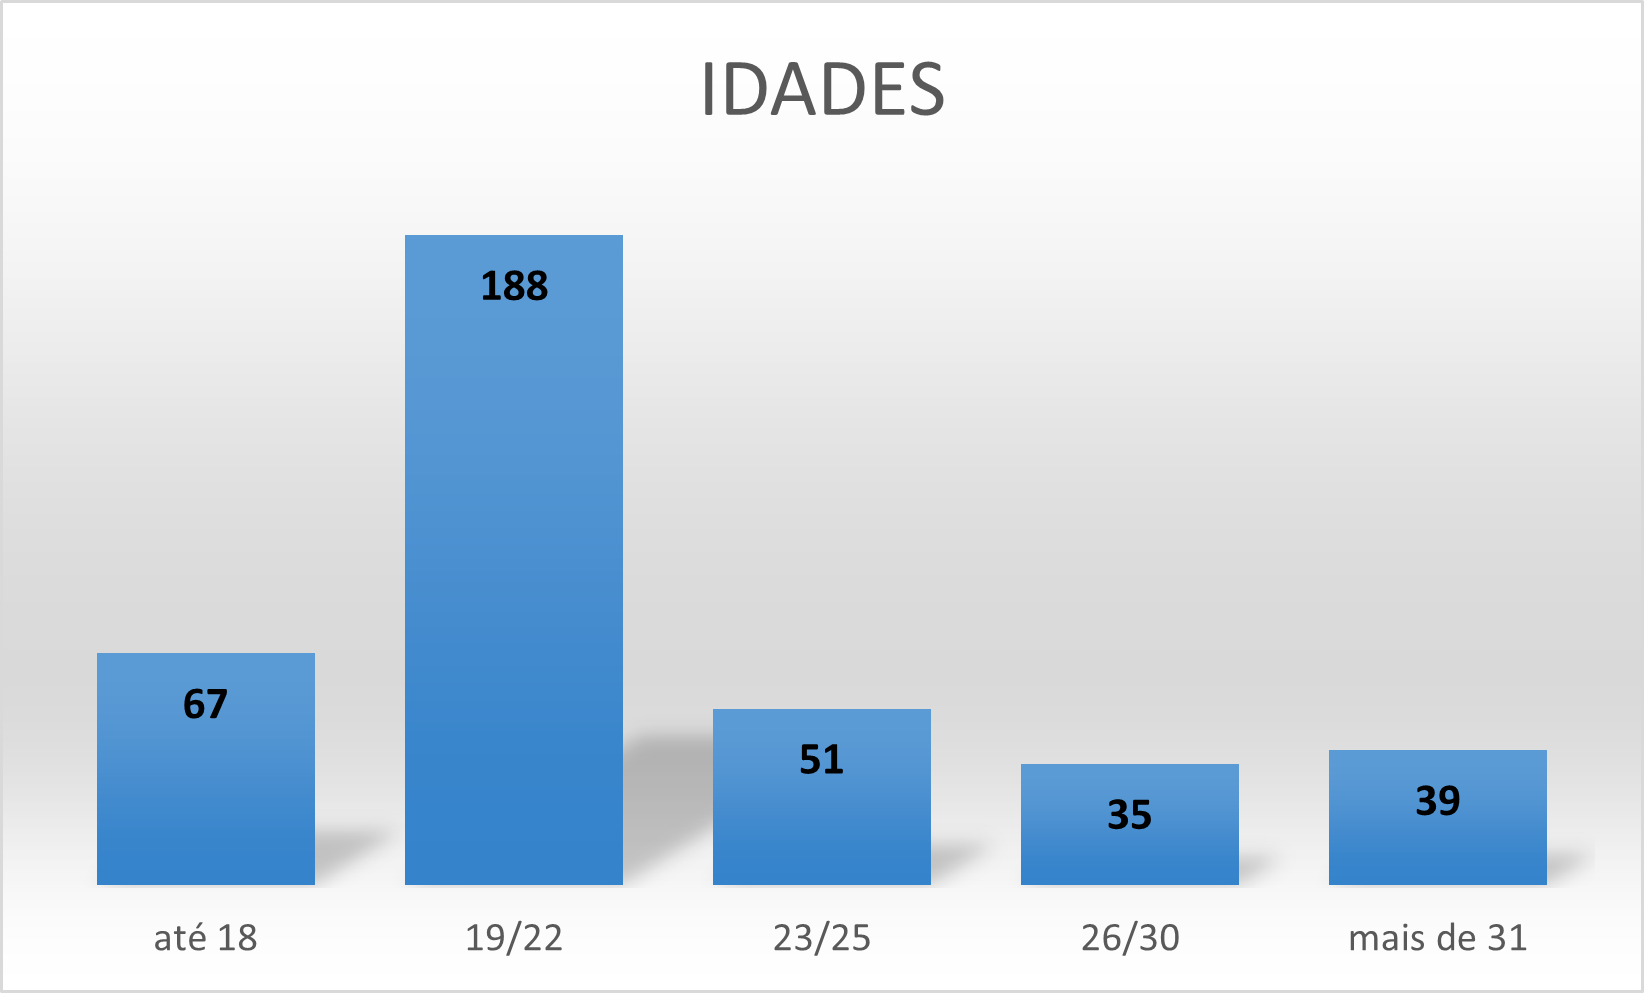
\includegraphics{figs/graph_idade.png}
            \captionof{figure}{Idade}
            \label{fig:graph_idade}
        \end{minipage}        
    \end{center}



    \item Tipo da Cidade

    A figura 2 descreve o tipo da cidade das pessoas respondentes da pesquisa.

    \vspace{\baselineskip}
    \begin{center}
        \begin{minipage}{\textwidth}
            %\centering
            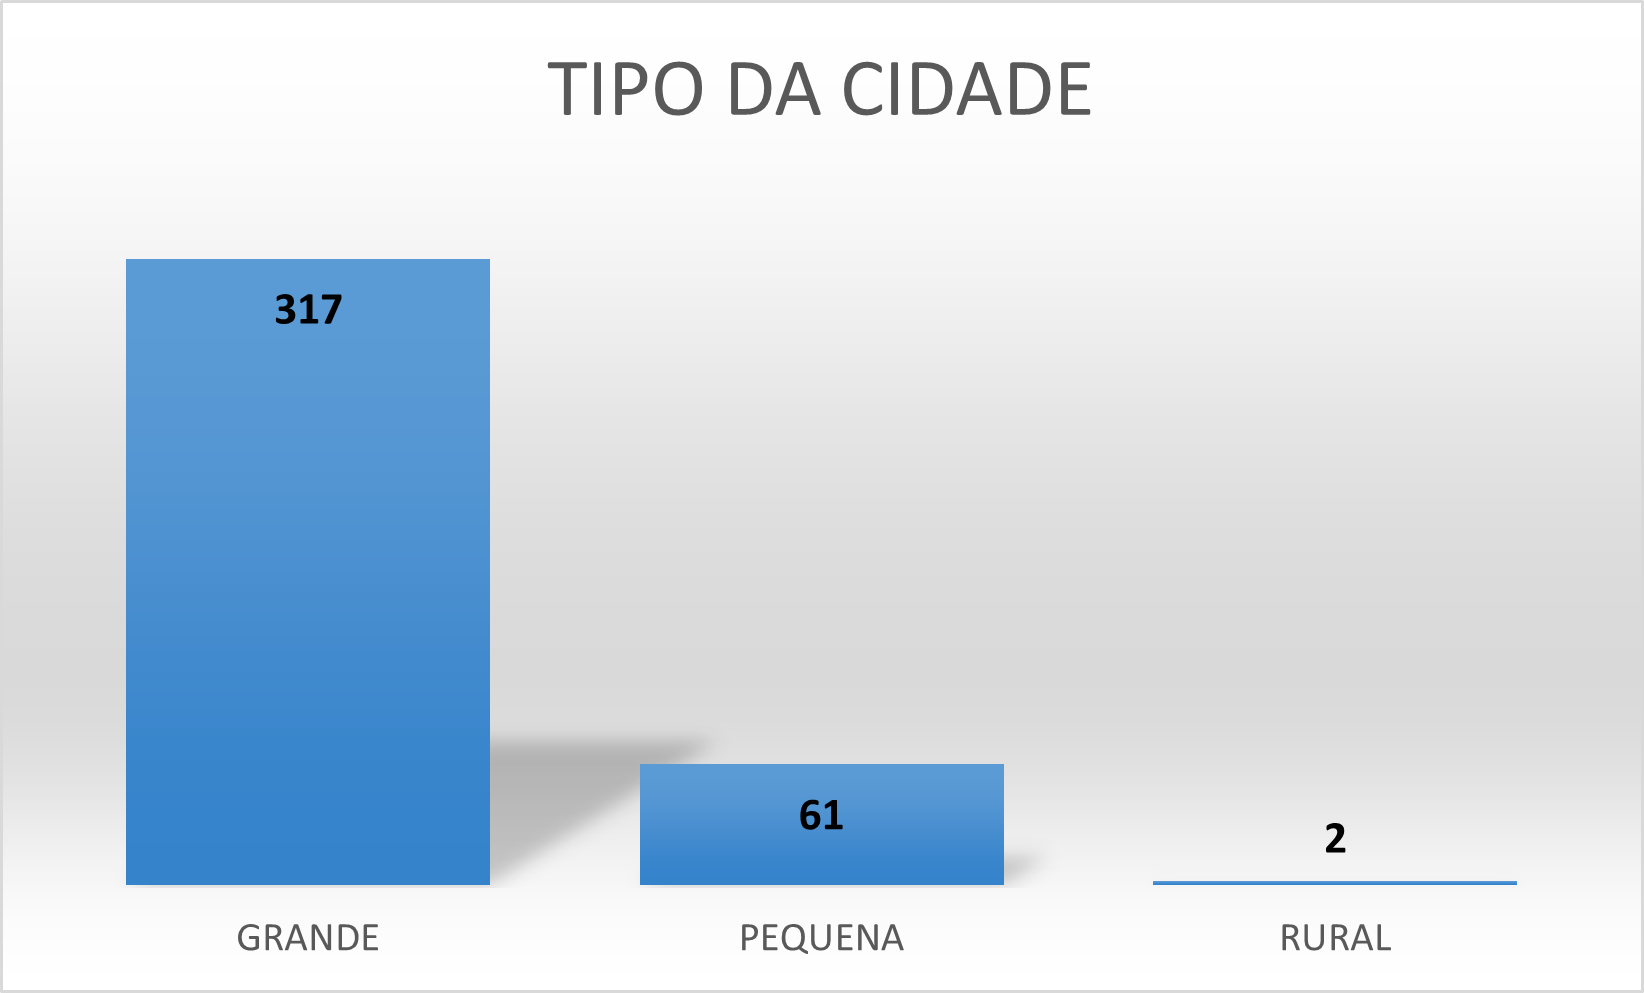
\includegraphics{figs/graph_cidade.png}
            \captionof{figure}{Tipo da Cidade}
            \label{fig:graph_cidade}
        \end{minipage}     
    \end{center}


    \vspace{\baselineskip}
    \vspace{\baselineskip}
    \item Formação

    A figura 3 descreve a formação das pessoas respondentes da pesquisa.

    \vspace{\baselineskip}
    \begin{center}
        \begin{minipage}{\textwidth}
            %\centering
            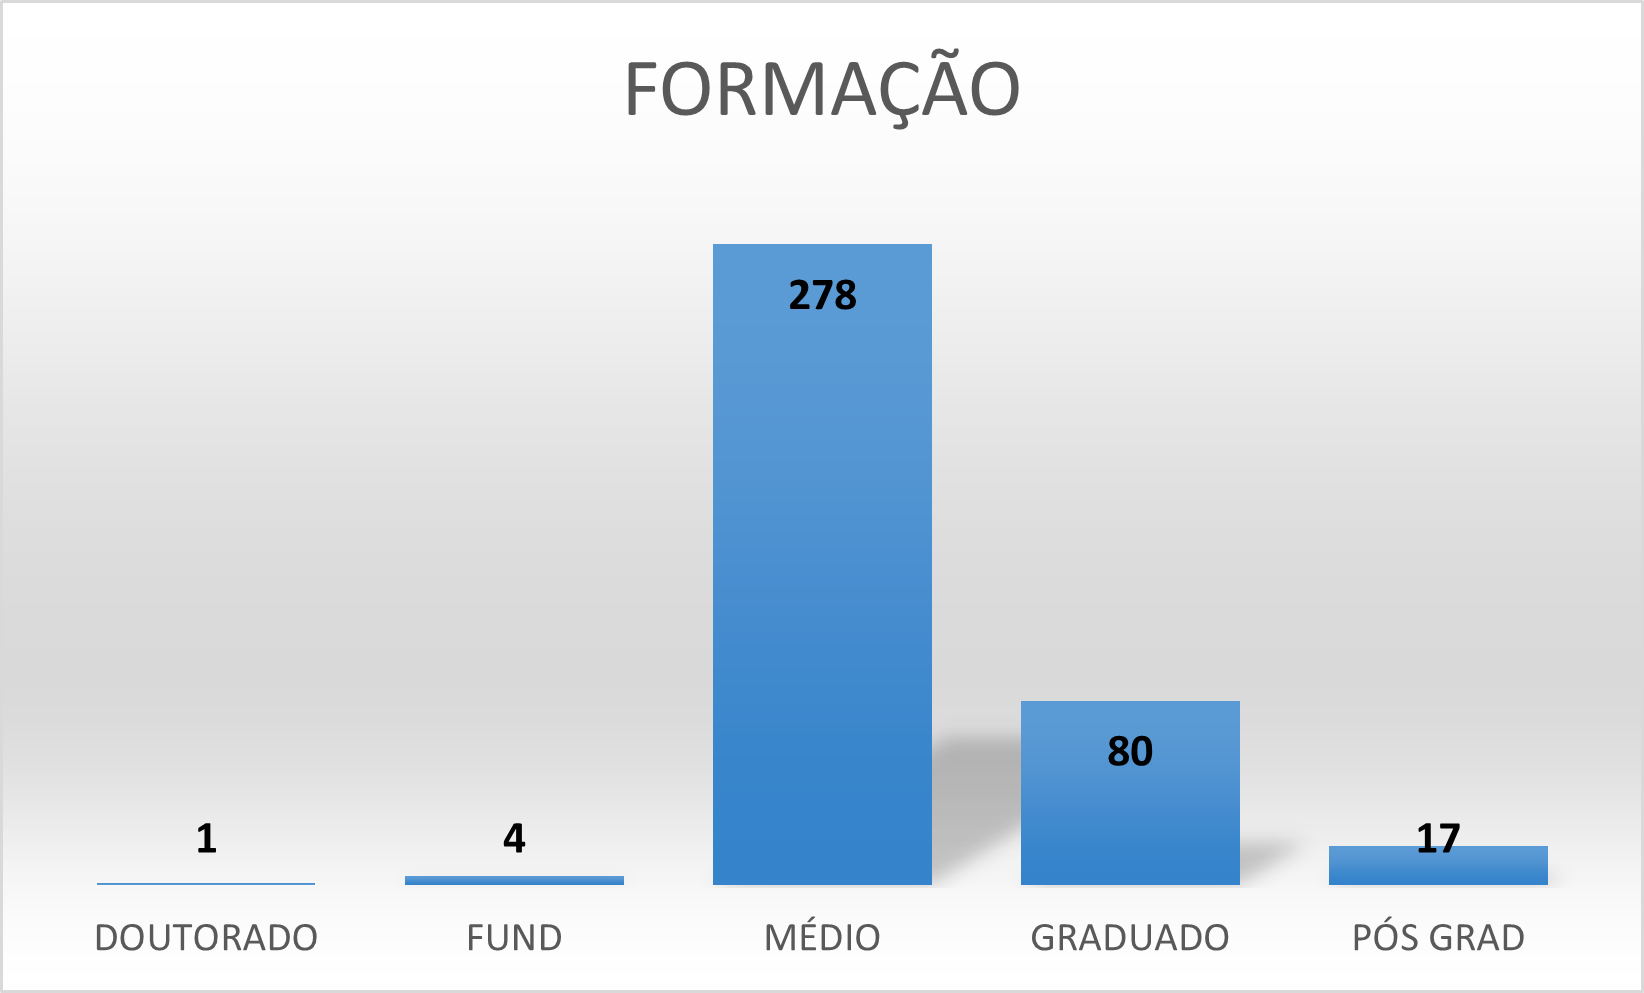
\includegraphics{figs/graph_formacao.png}
            \captionof{figure}{Formação}
            \label{fig:graph_formacao}
        \end{minipage}        
    \end{center}

    \item Renda (em Reais)

    A figura 4 descreve a renda das pessoas respondentes da pesquisa.

    \vspace{\baselineskip}
    \begin{center}
        \begin{minipage}{\textwidth}
            %\centering
            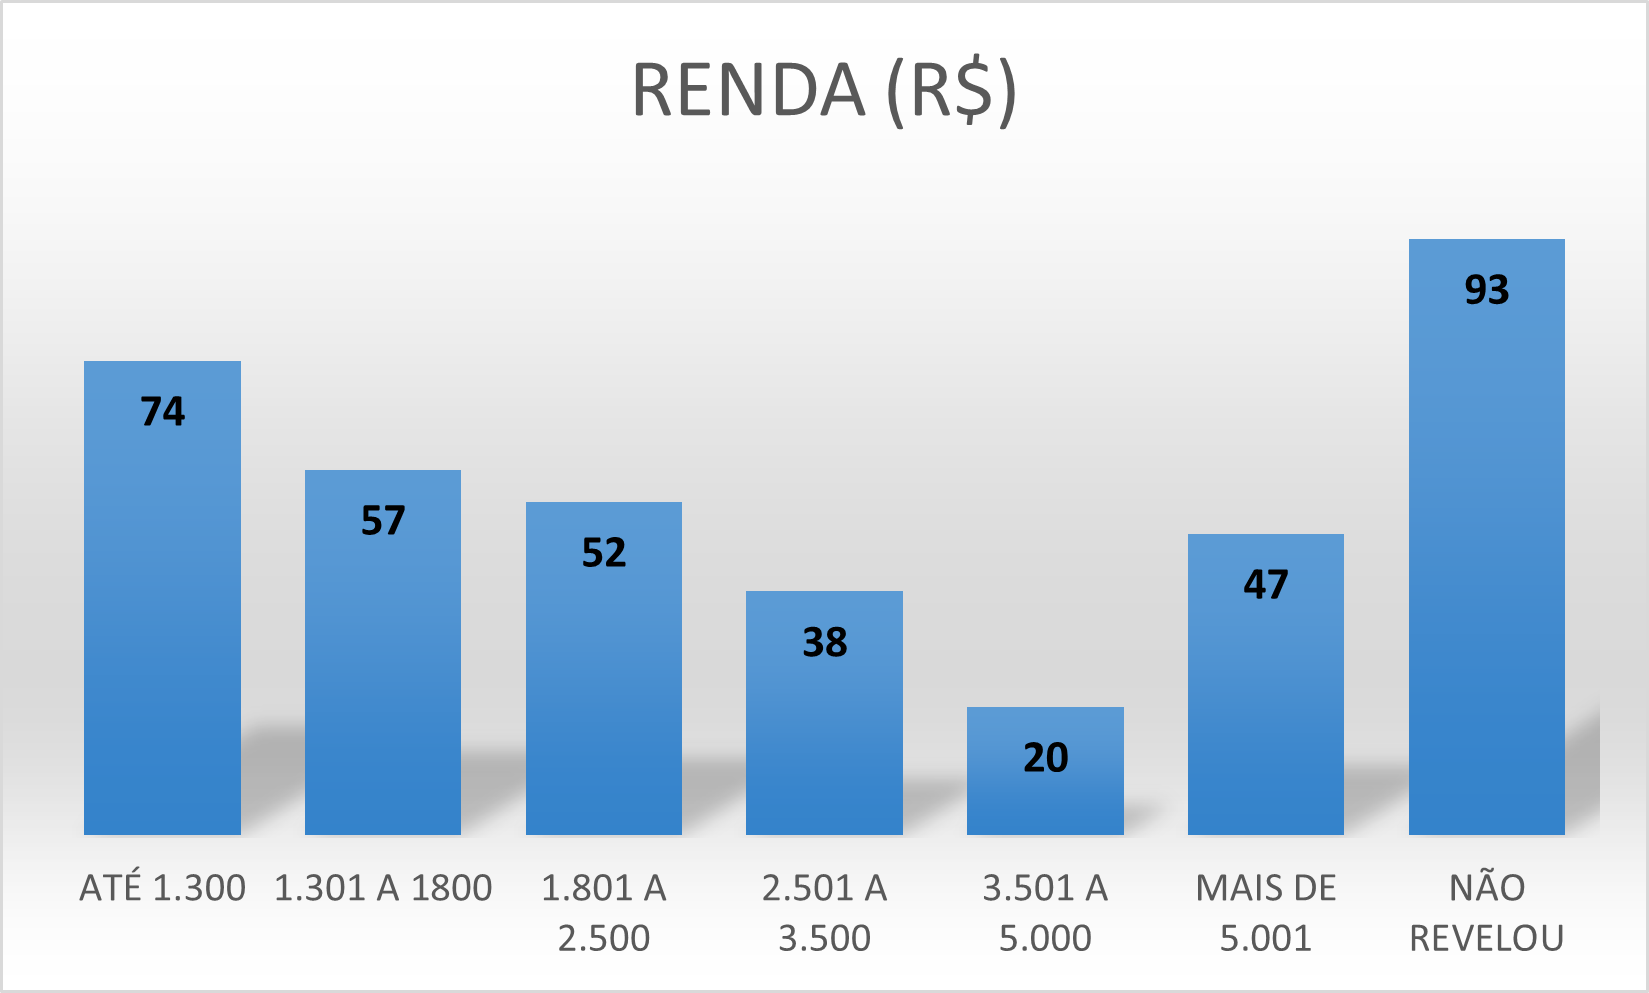
\includegraphics{figs/graph_renda.png}
            \captionof{figure}{Renda}
            \label{fig:graph_renda}
        \end{minipage}        
    \end{center}

    \vspace{\baselineskip}
    \vspace{\baselineskip}
    \vspace{\baselineskip}
    \vspace{\baselineskip}
    \vspace{\baselineskip}
    \item Situação Financeira

    A figura 5 descreve a situação financeira das pessoas respondentes da pesquisa.

    \vspace{\baselineskip}
    \begin{center}
        \begin{minipage}{\textwidth}
            %\centering
            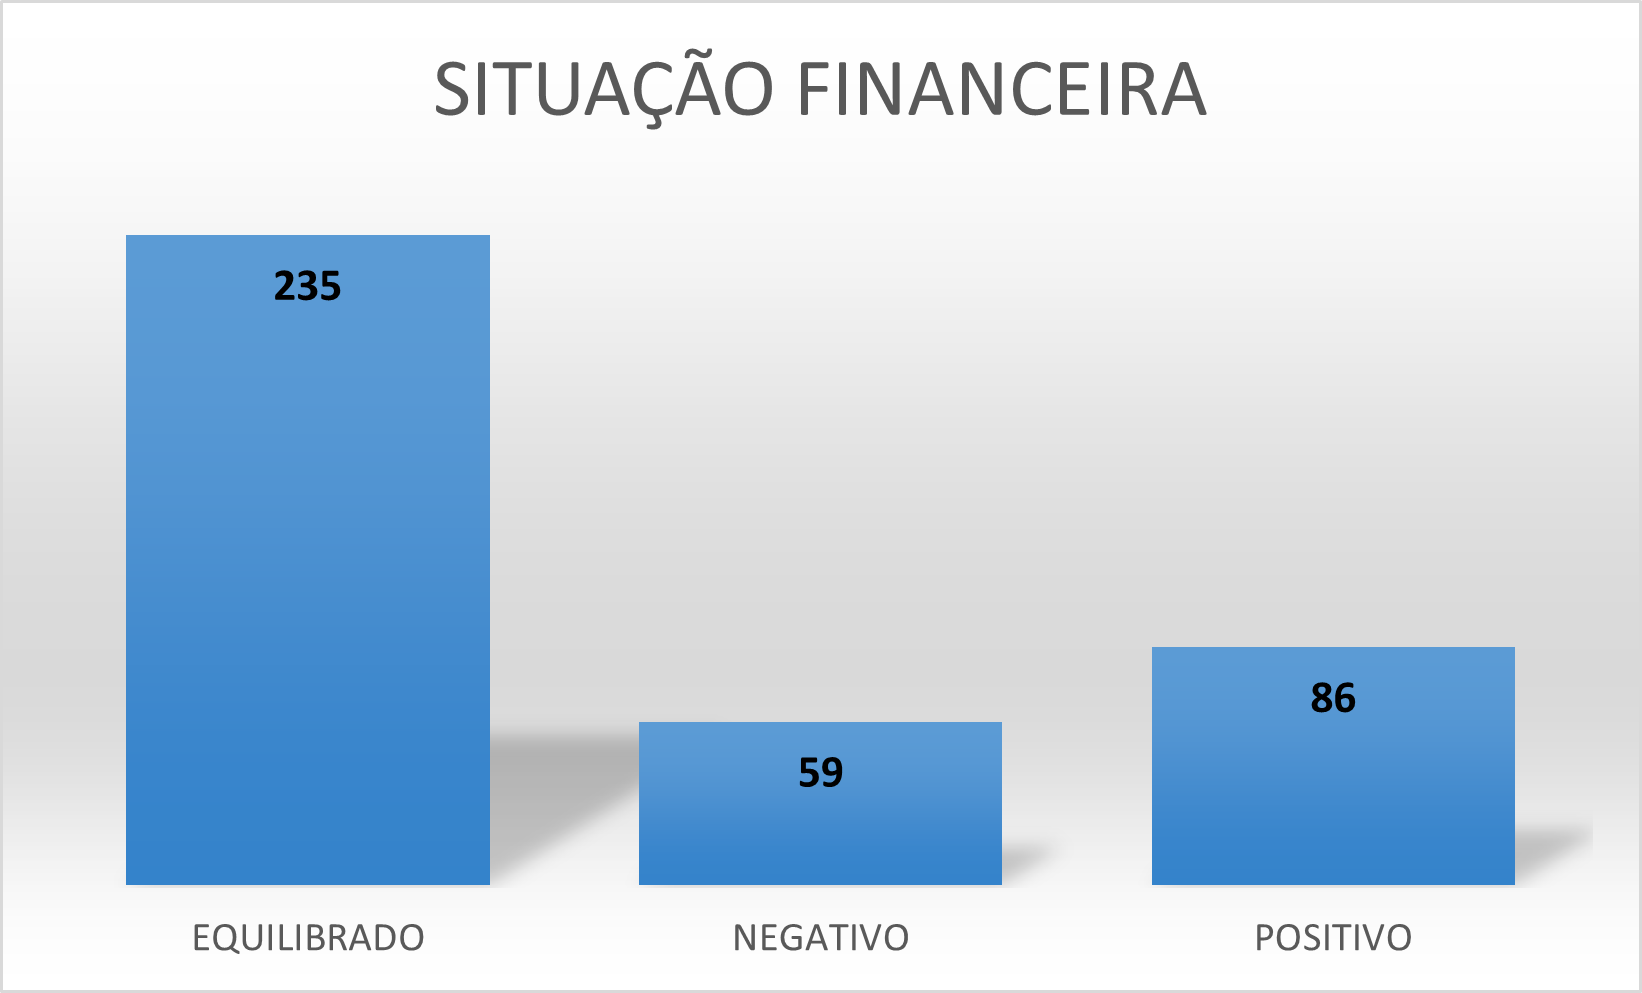
\includegraphics{figs/graph_situacao.png}
            \captionof{figure}{Situação Financeira}
            \label{fig:graph_situacao}
        \end{minipage}        
    \end{center}


    \item Educação Financeira

    A figura 6 descreve a educação financeira das pessoas respondentes da pesquisa.

    \vspace{\baselineskip}
    \begin{center}
        \begin{minipage}{\textwidth}
            %\centering
            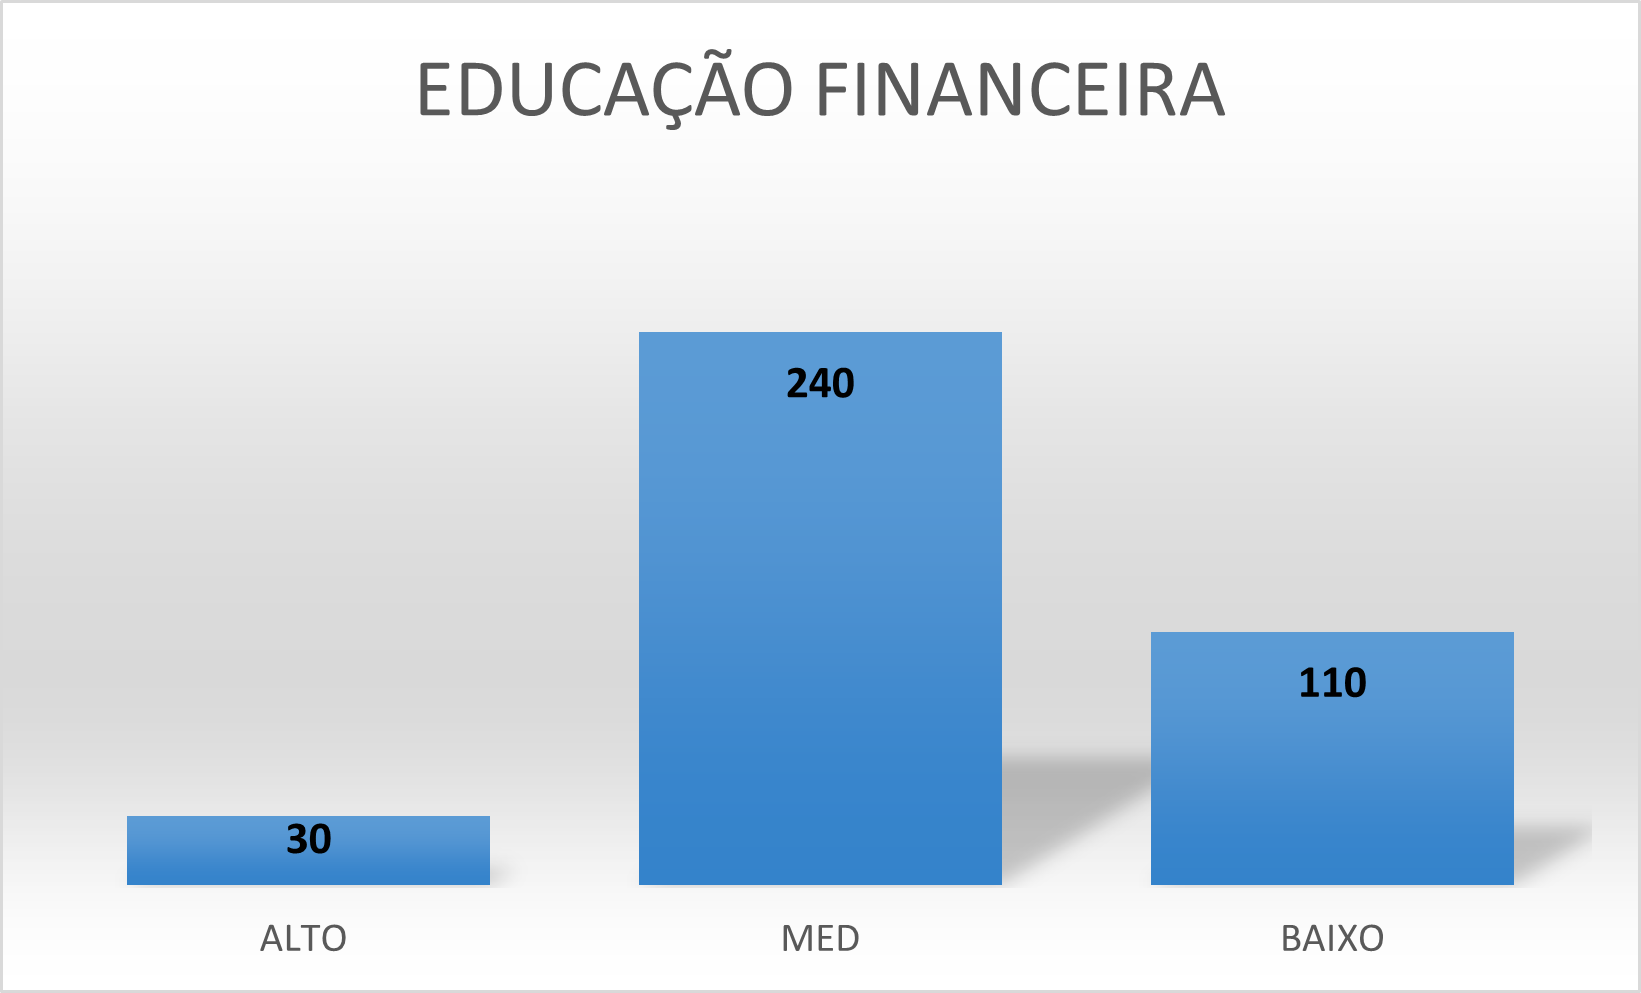
\includegraphics{figs/graph_educacao.png}
            \captionof{figure}{Educação Financeira}
            \label{fig:graph_educacao}
        \end{minipage}       
    \end{center}


    \vspace{\baselineskip}
    \vspace{\baselineskip}
    \vspace{\baselineskip}
    \vspace{\baselineskip}
    \vspace{\baselineskip}
    \vspace{\baselineskip}
    \item Possui Algum Crédito?

    A figura 7 descreve a existência de algum crédito das pessoas respondentes da pesquisa.

    \vspace{\baselineskip}
    \begin{center}
        \begin{minipage}{\textwidth}
            %\centering
            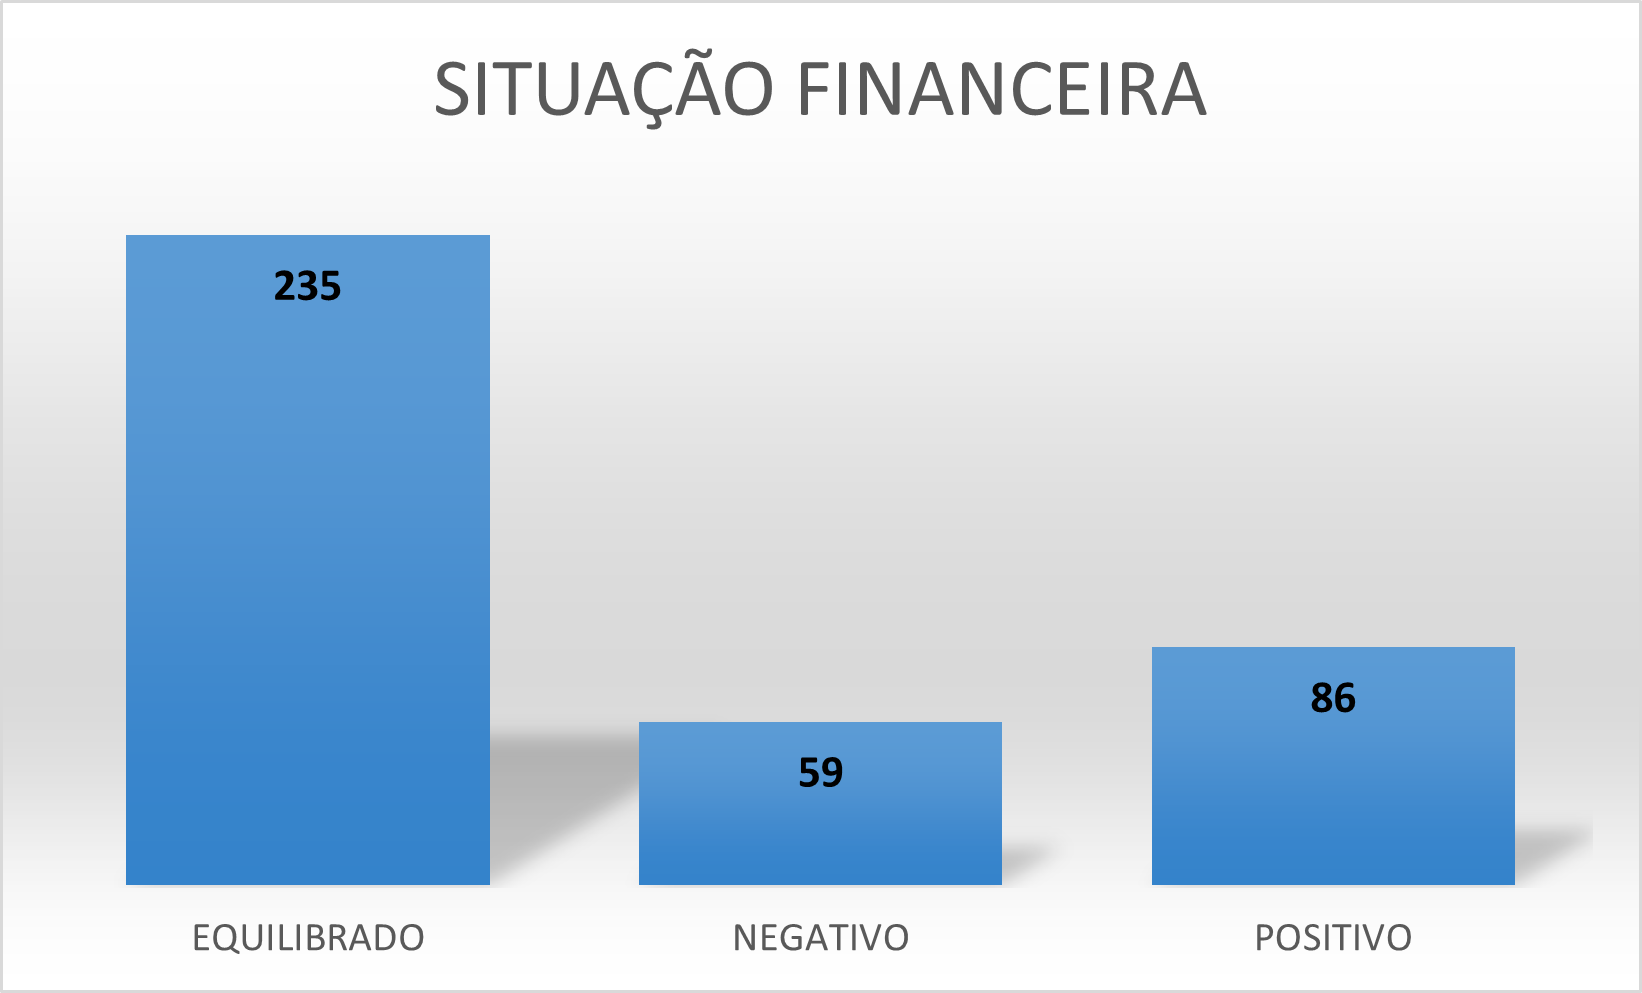
\includegraphics{figs/graph_situacao.png}
            \captionof{figure}{Possui Algum Credito?}
            \label{fig:graph_situacao}
        \end{minipage}        
    \end{center}


    \item Tipo de Crédito

    A figura 8 descreve o tipo de crédito das pessoas respondentes da pesquisa.

    \vspace{\baselineskip}
    \begin{center}
        \begin{minipage}{\textwidth}
            %\centering
            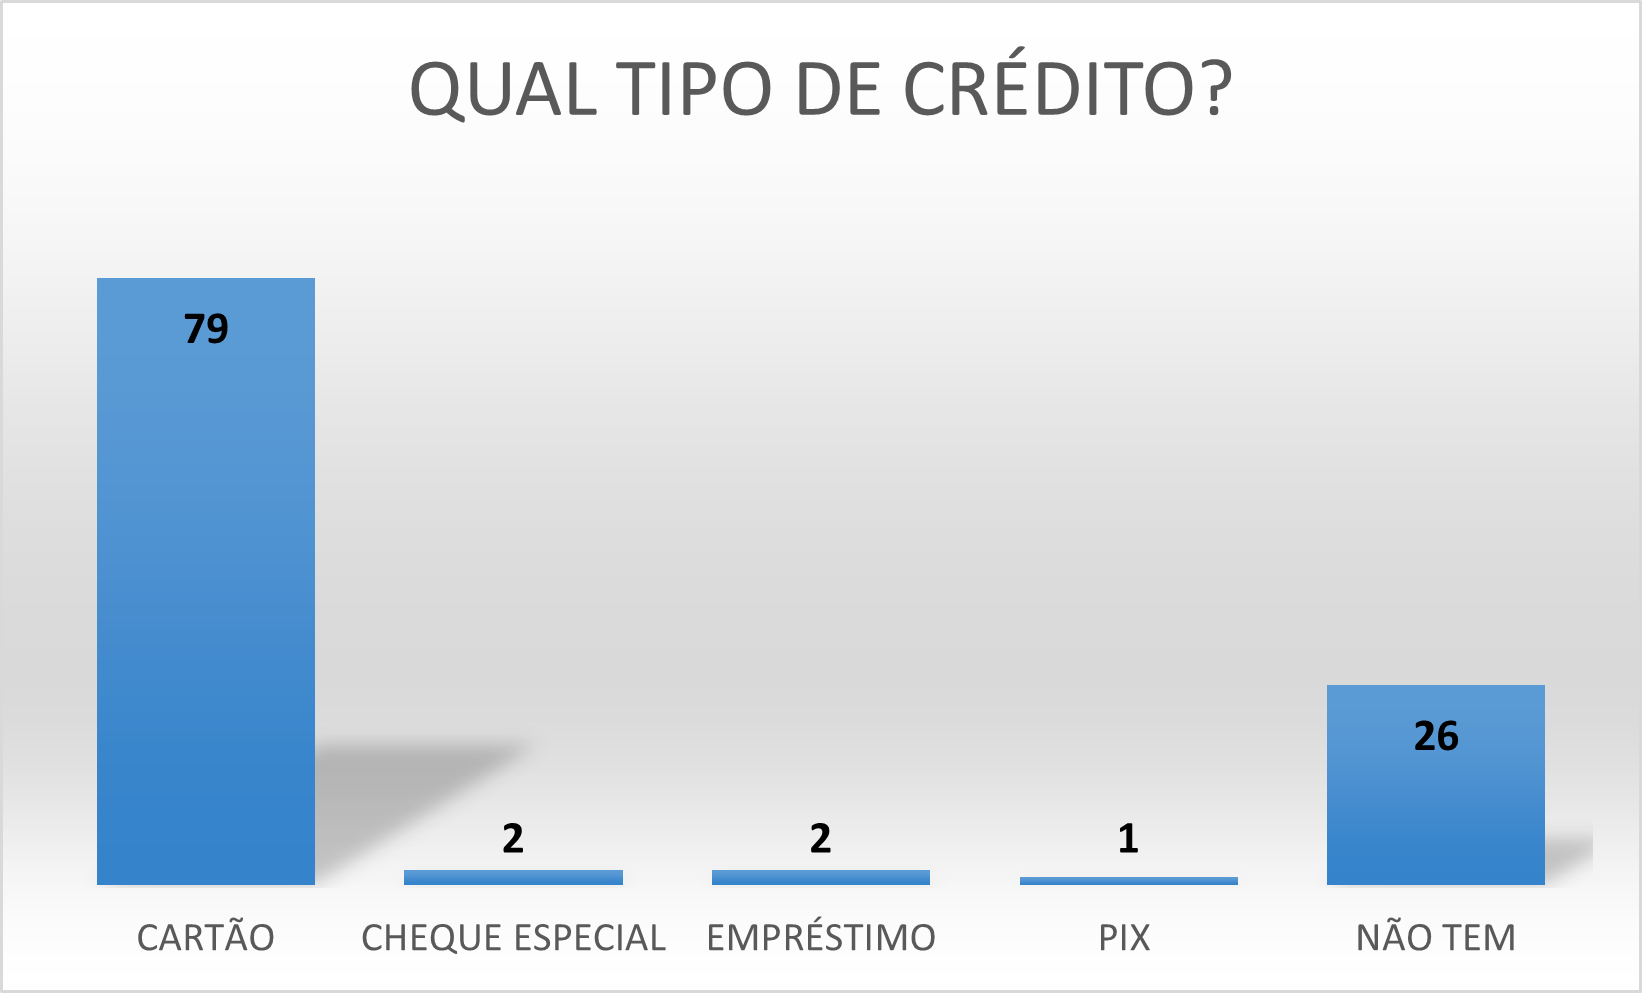
\includegraphics{figs/graph_tipo-credito.png}
            \captionof{figure}{Tipo de Crédito}
            \label{fig:graph_tipo-credito}
        \end{minipage}   
    \end{center}


    \vspace{\baselineskip}
    \vspace{\baselineskip}
    \vspace{\baselineskip}
    \vspace{\baselineskip}
    \item Método Mais Utilizado

    A figura 9 descreve o método mais utilizado das pessoas respondentes da pesquisa.

    \vspace{\baselineskip}
    \begin{center}
        \begin{minipage}{\textwidth}
           %\centering
            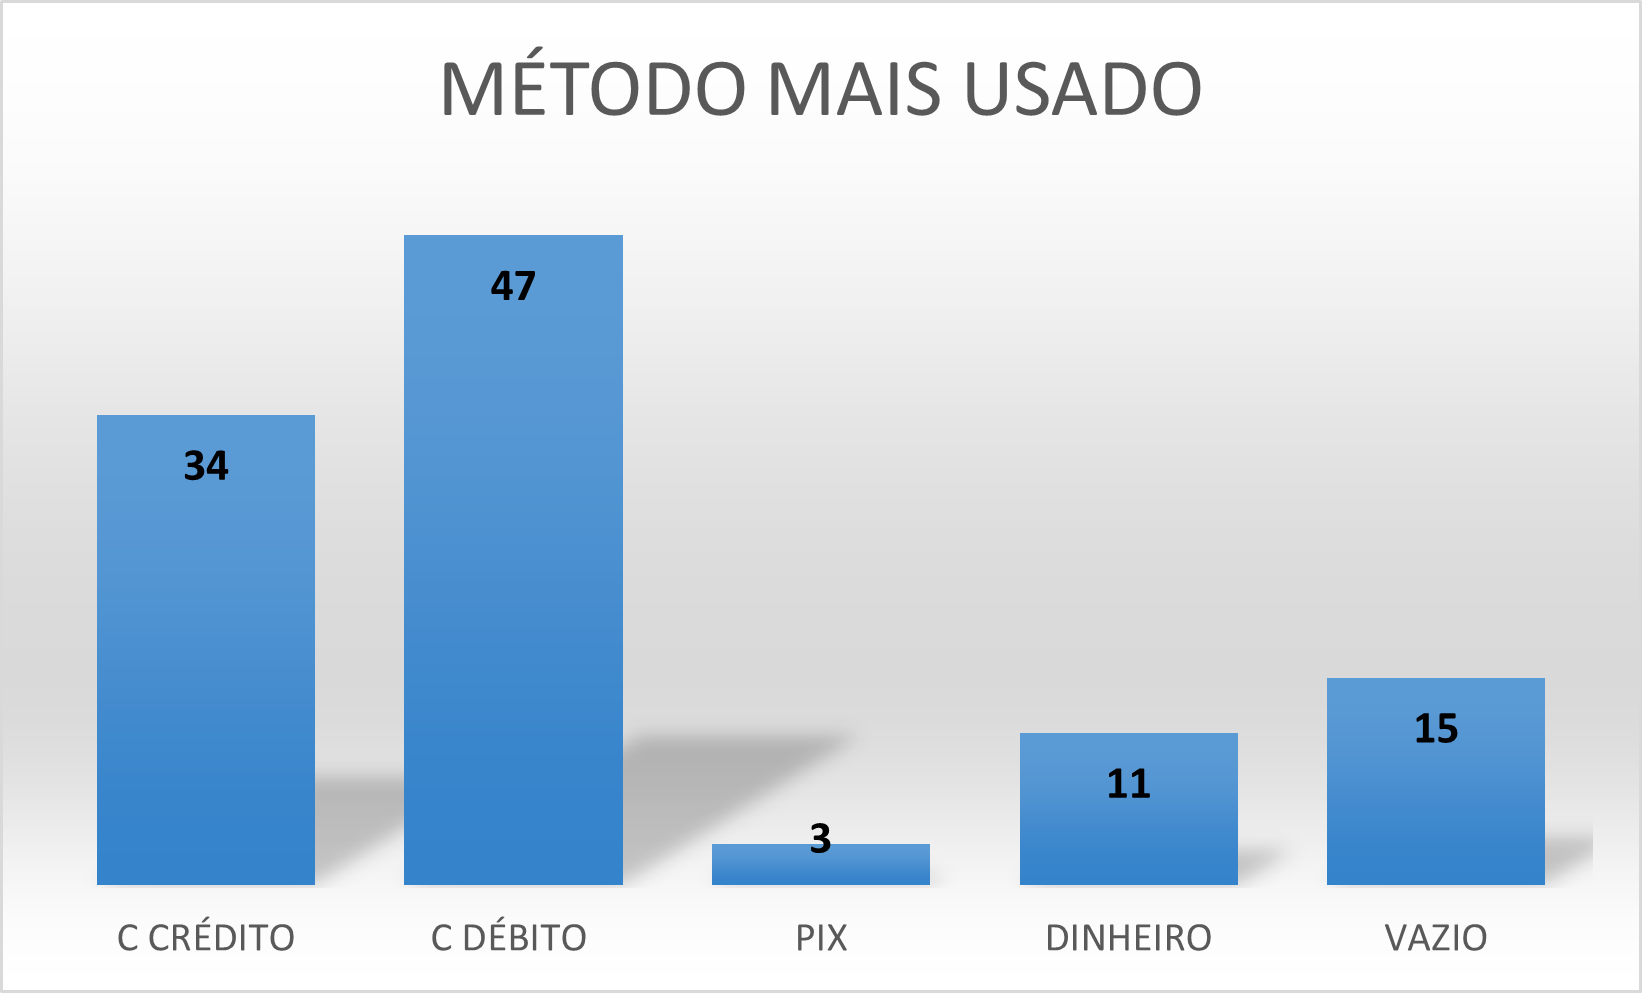
\includegraphics{figs/graph_mais-usado.png}
            \captionof{figure}{ Método Mais Utilizado}
            \label{fig:graph_mais-usado}
        \end{minipage}        
    \end{center}

    \item Se Considera Organizado?

    A figura 10 descreve Se Considera Organizado?, das pessoas respondentes da pesquisa.

    \vspace{\baselineskip}
    \begin{center}
        \begin{minipage}{\textwidth}
            %\centering
            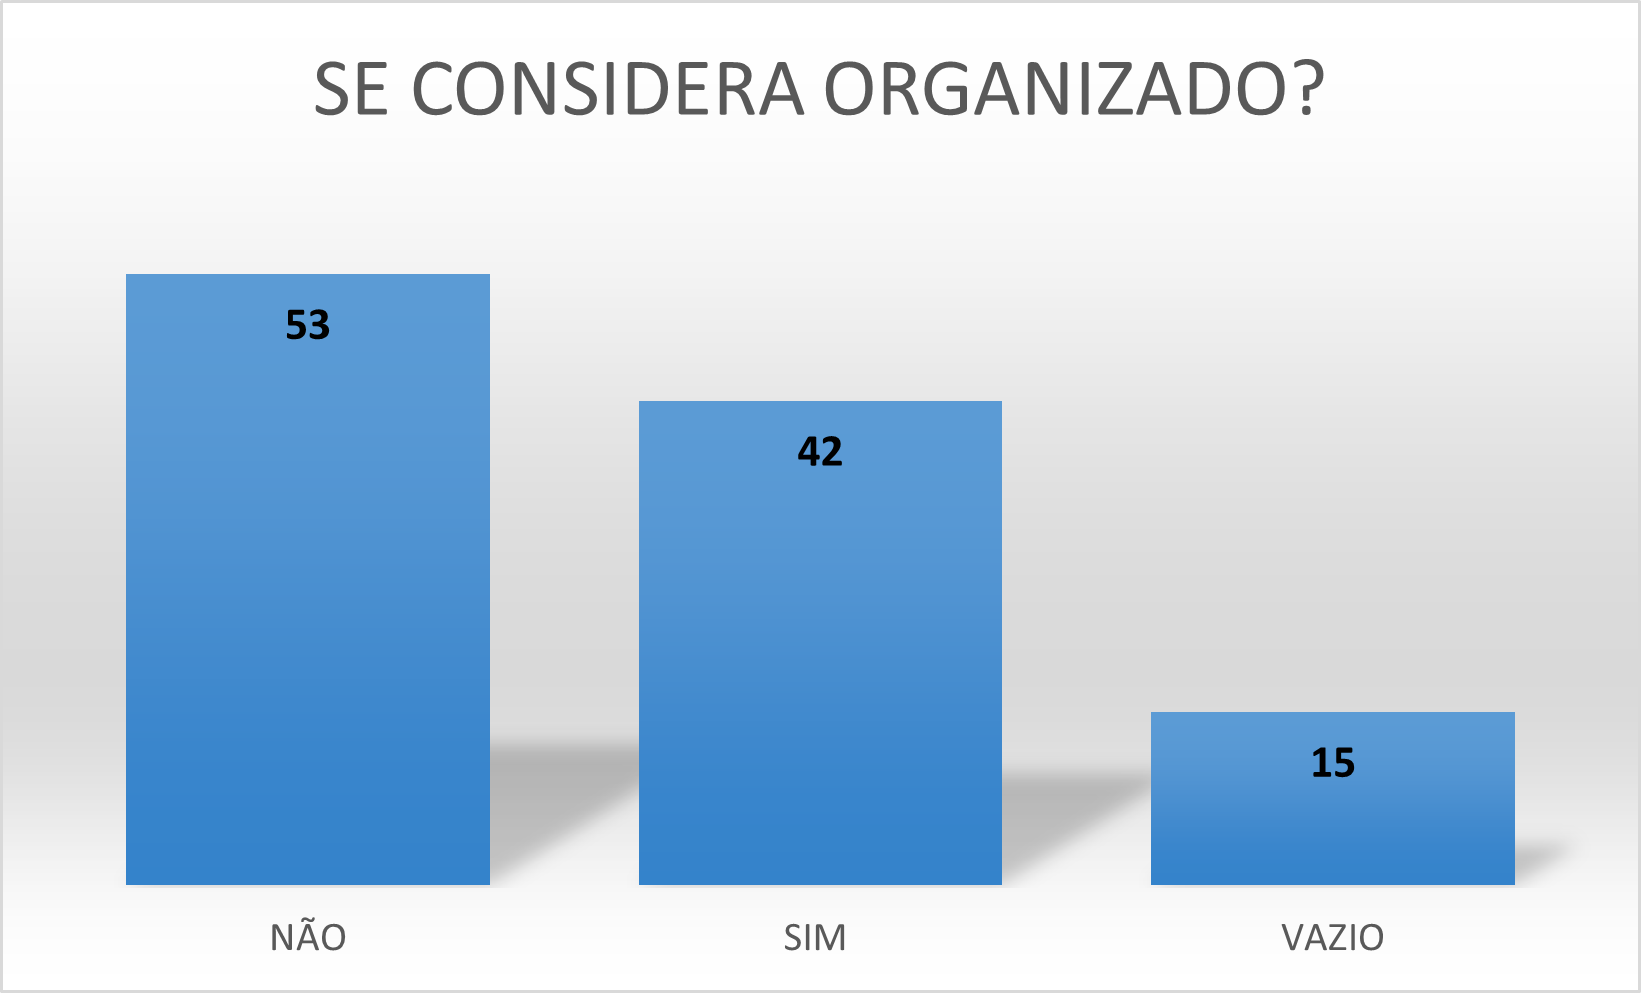
\includegraphics{figs/graph_considera-organizado.png}
            \captionof{figure}{Se Considera Organizado?}
            \label{fig:graph_considera-organizado}
        \end{minipage}        
    \end{center}
    
\end{enumerate}

% ----------------------------------------------------------
% Análise dos Resultados
% 
% ----------------------------------------------------------

\chapter[Desenvolvimento]{Desenvolvimento}

A pesquisa realizada proporcionou uma compreensão mais profunda dos potenciais clientes e usuários da solução, os quais são, no caso, jovens entre 19 e 22 anos. No contexto, os clientes e os usuários da solução são as mesmas pessoas, já que quem paga é também quem utiliza. Portanto, devido à inexistência de distinção entre usuários e clientes, a implementação do MVP é única.

\section{Requisitos do Sistema}
Como usuário do aplicativo FiMa, quero poder gerenciar minhas finanças de forma prática e transparente, tendo uma visão geral das despesas e receitas, podendo definir e acompanhar metas, recebendo sugestões de melhoria com base nos meus dados, para que eu atinja minhas metas e objetivos.

\subsection{Estória do Painel de Visão Geral}
Como usuário do aplicativo FiMa, quero ver um painel de visão geral das minhas finanças que exiba meu saldo atual, despesas, receitas e histórico, para ter melhor visibilidade.

\subsection{Estória de Definição de Metas}
Como usuário do aplicativo FiMa, quero poder definir metas financeiras, como economizar para uma viagem, um carro novo ou uma emergência, para que eu possa acompanhar meu progresso em relação a essas metas.

\subsection{Estória de Acompanhamento de Metas}
Como usuário do aplicativo FiMa, quero ser capaz de acompanhar meu progresso em relação às metas financeiras definidas, recebendo atualizações regulares sobre o quanto já alcancei e o que falta para atingir cada meta.

\subsection{Estória de Categorização de Despesas e Receitas}
Como usuário do aplicativo FiMa, quero poder categorizar minhas despesas e receitas, para que eu possa entender melhor para onde meu dinheiro está indo.

\subsection{Estória de Segurança e Privacidade}
Como usuário do aplicativo FiMa, quero ter a garantia de que meus dados financeiros serão protegidos adequadamente e que a privacidade das minhas informações será respeitada em conformidade com a Lei Geral de Proteção de Dados.

\section{Cronograma de Projeto}

Diagrama de Gantt contendo as atividades, papéis e responsabilidades dos participantes do grupo, conforme descrito na figura 11.

    \vspace{\baselineskip}
    \begin{center}
        \begin{minipage}{\textwidth}
            %\centering
            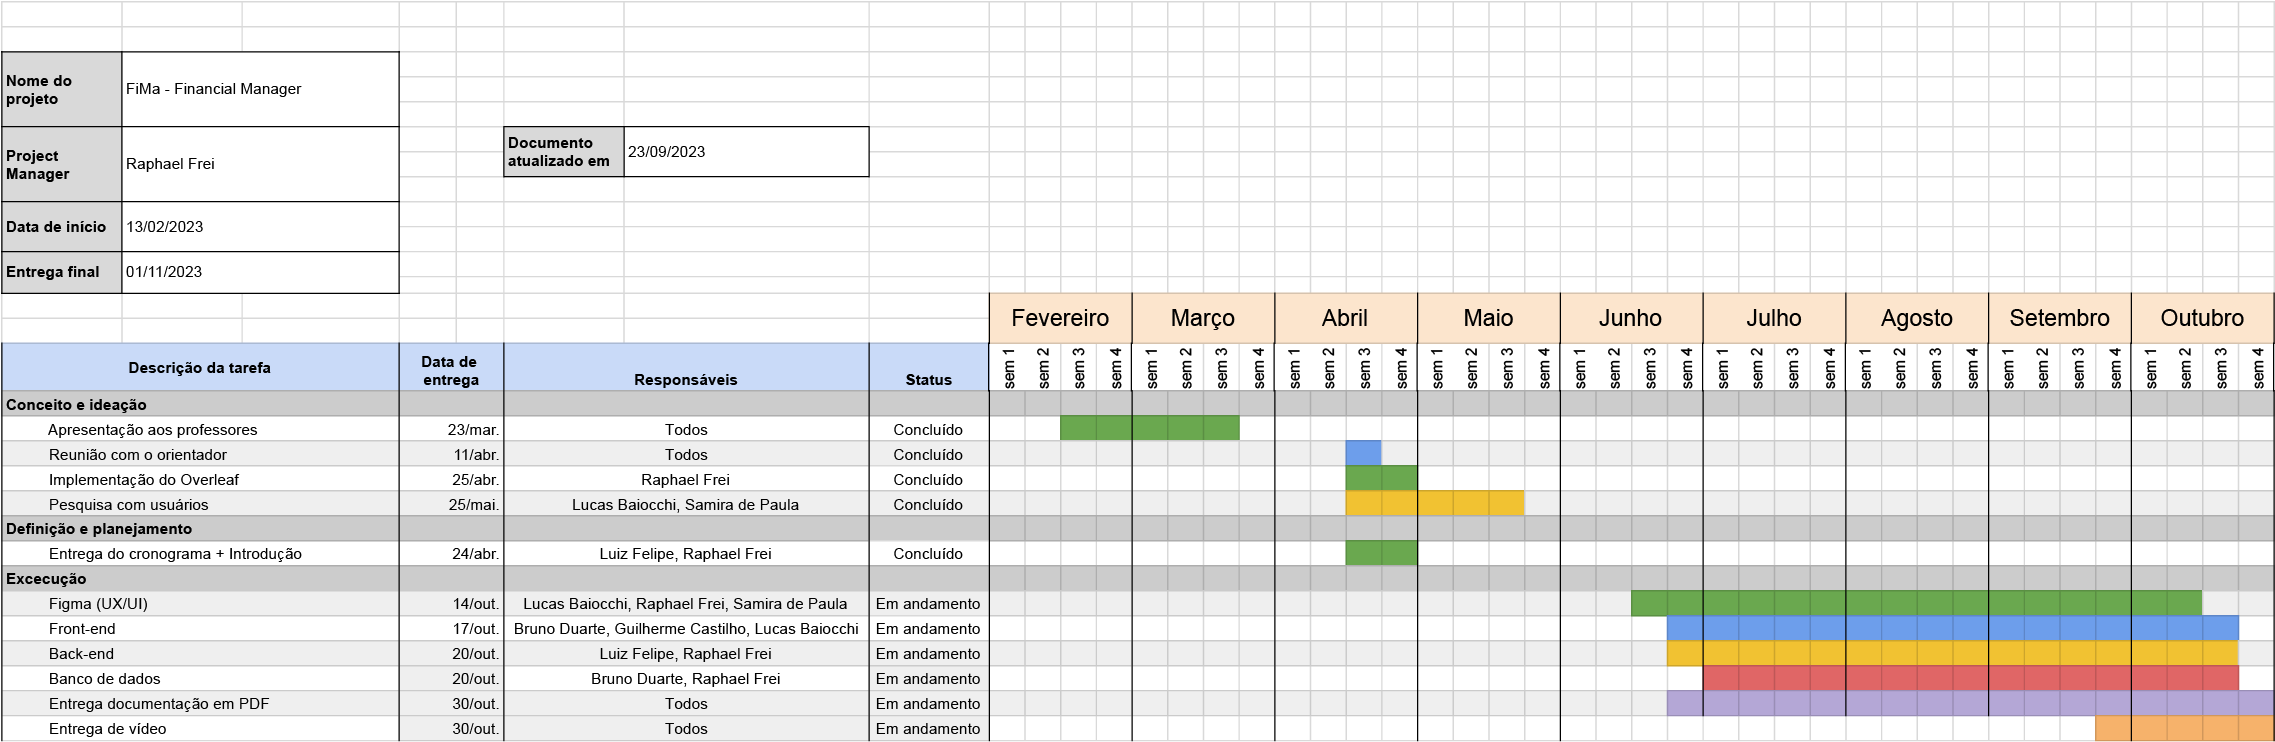
\includegraphics[scale=0.35]{figs/gantt.png}
            \captionof{figure}{Gráfico de Gantt}
            \label{fig:gantt}
        \end{minipage}
    \end{center}
    

\section{Desenho da Arquitetura do Software}

A figura 12 abaixo contém a arquitetura geral do sistema.

    \vspace{\baselineskip}
    \begin{center}
        \begin{minipage}{\textwidth}
            \centering
            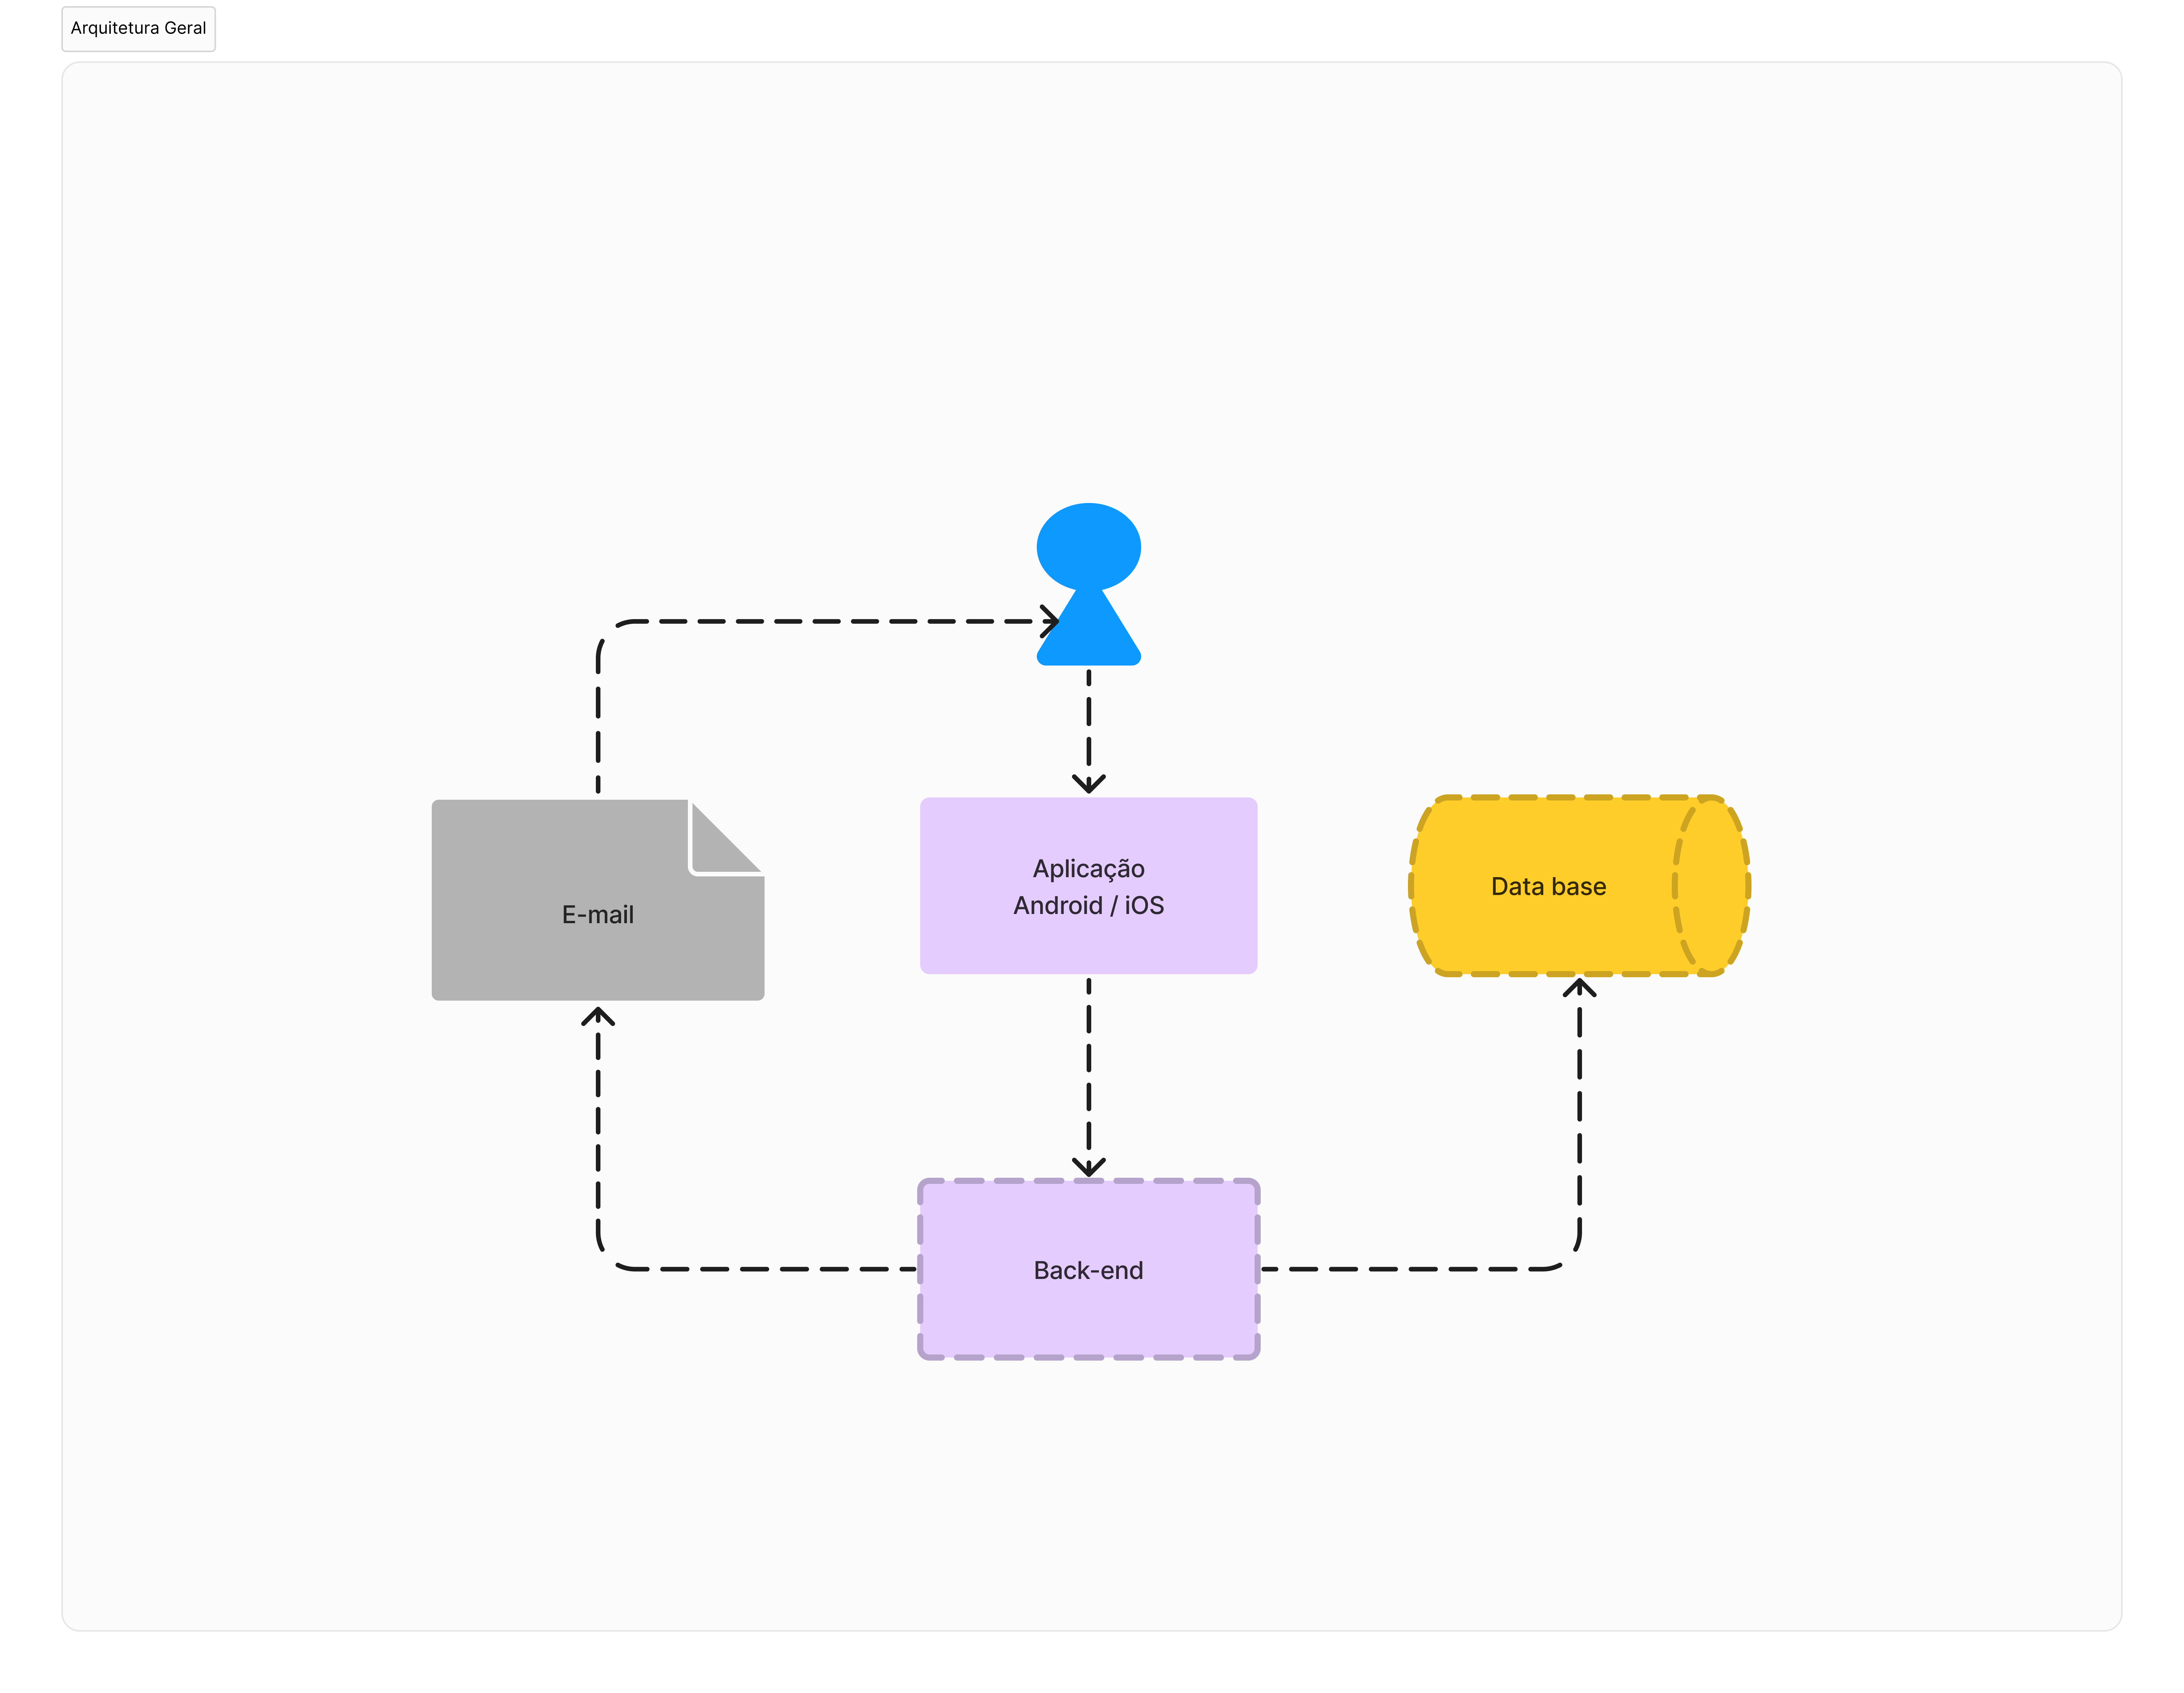
\includegraphics[scale=0.17]{figs/arq_geral.png}
            \captionof{figure}{Arquitetura de Software}
            \label{fig:arq-geral}
        \end{minipage}
    \end{center}

A figura 13 abaixo contém a arquitetura específica do sistema.

    \vspace{\baselineskip}
    \begin{center}
        \begin{minipage}{\textwidth}
            \centering
            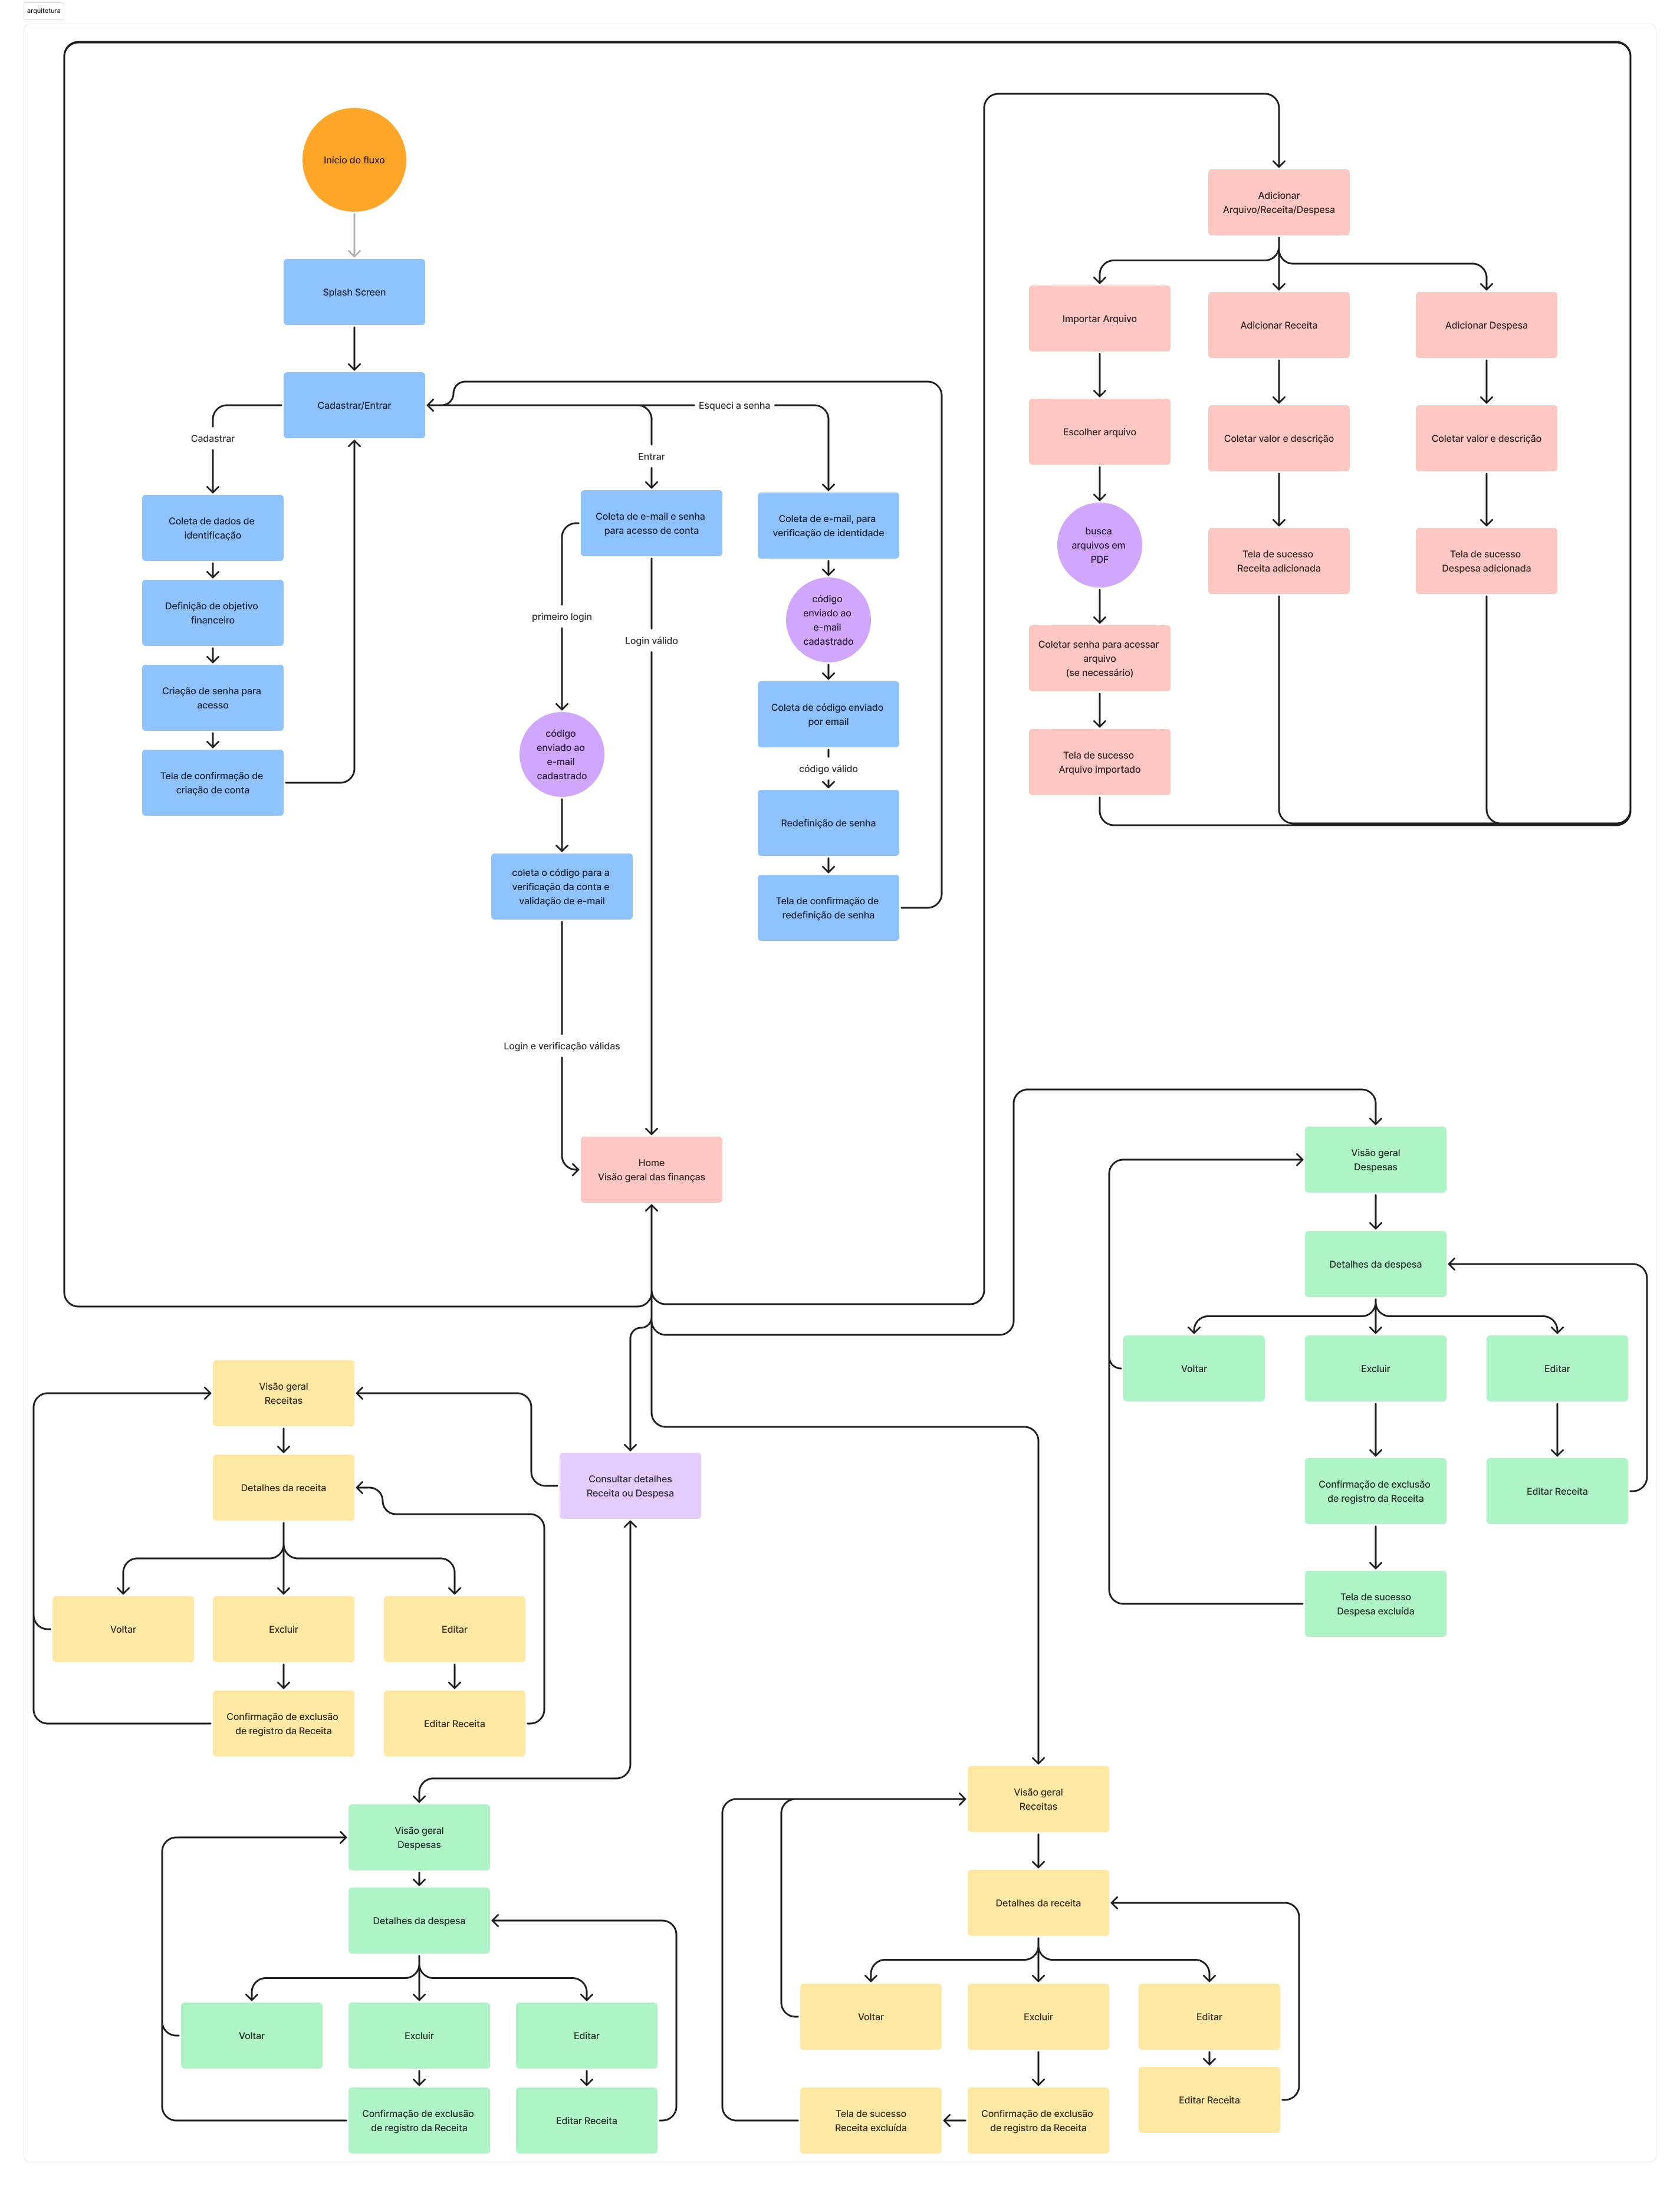
\includegraphics[scale=0.08]{figs/figura13.png}
            \captionof{figure}{Arquitetura Específica do Sistema}
            \label{fig:figura13}
        \end{minipage}
    \end{center}

\section{Desenho do Projeto de Banco de Dados}

Na figura 14 é apresentado o desenho do projeto do banco de dados.

    \vspace{\baselineskip}
    \begin{center}
        \begin{minipage}{\textwidth}
            \centering
            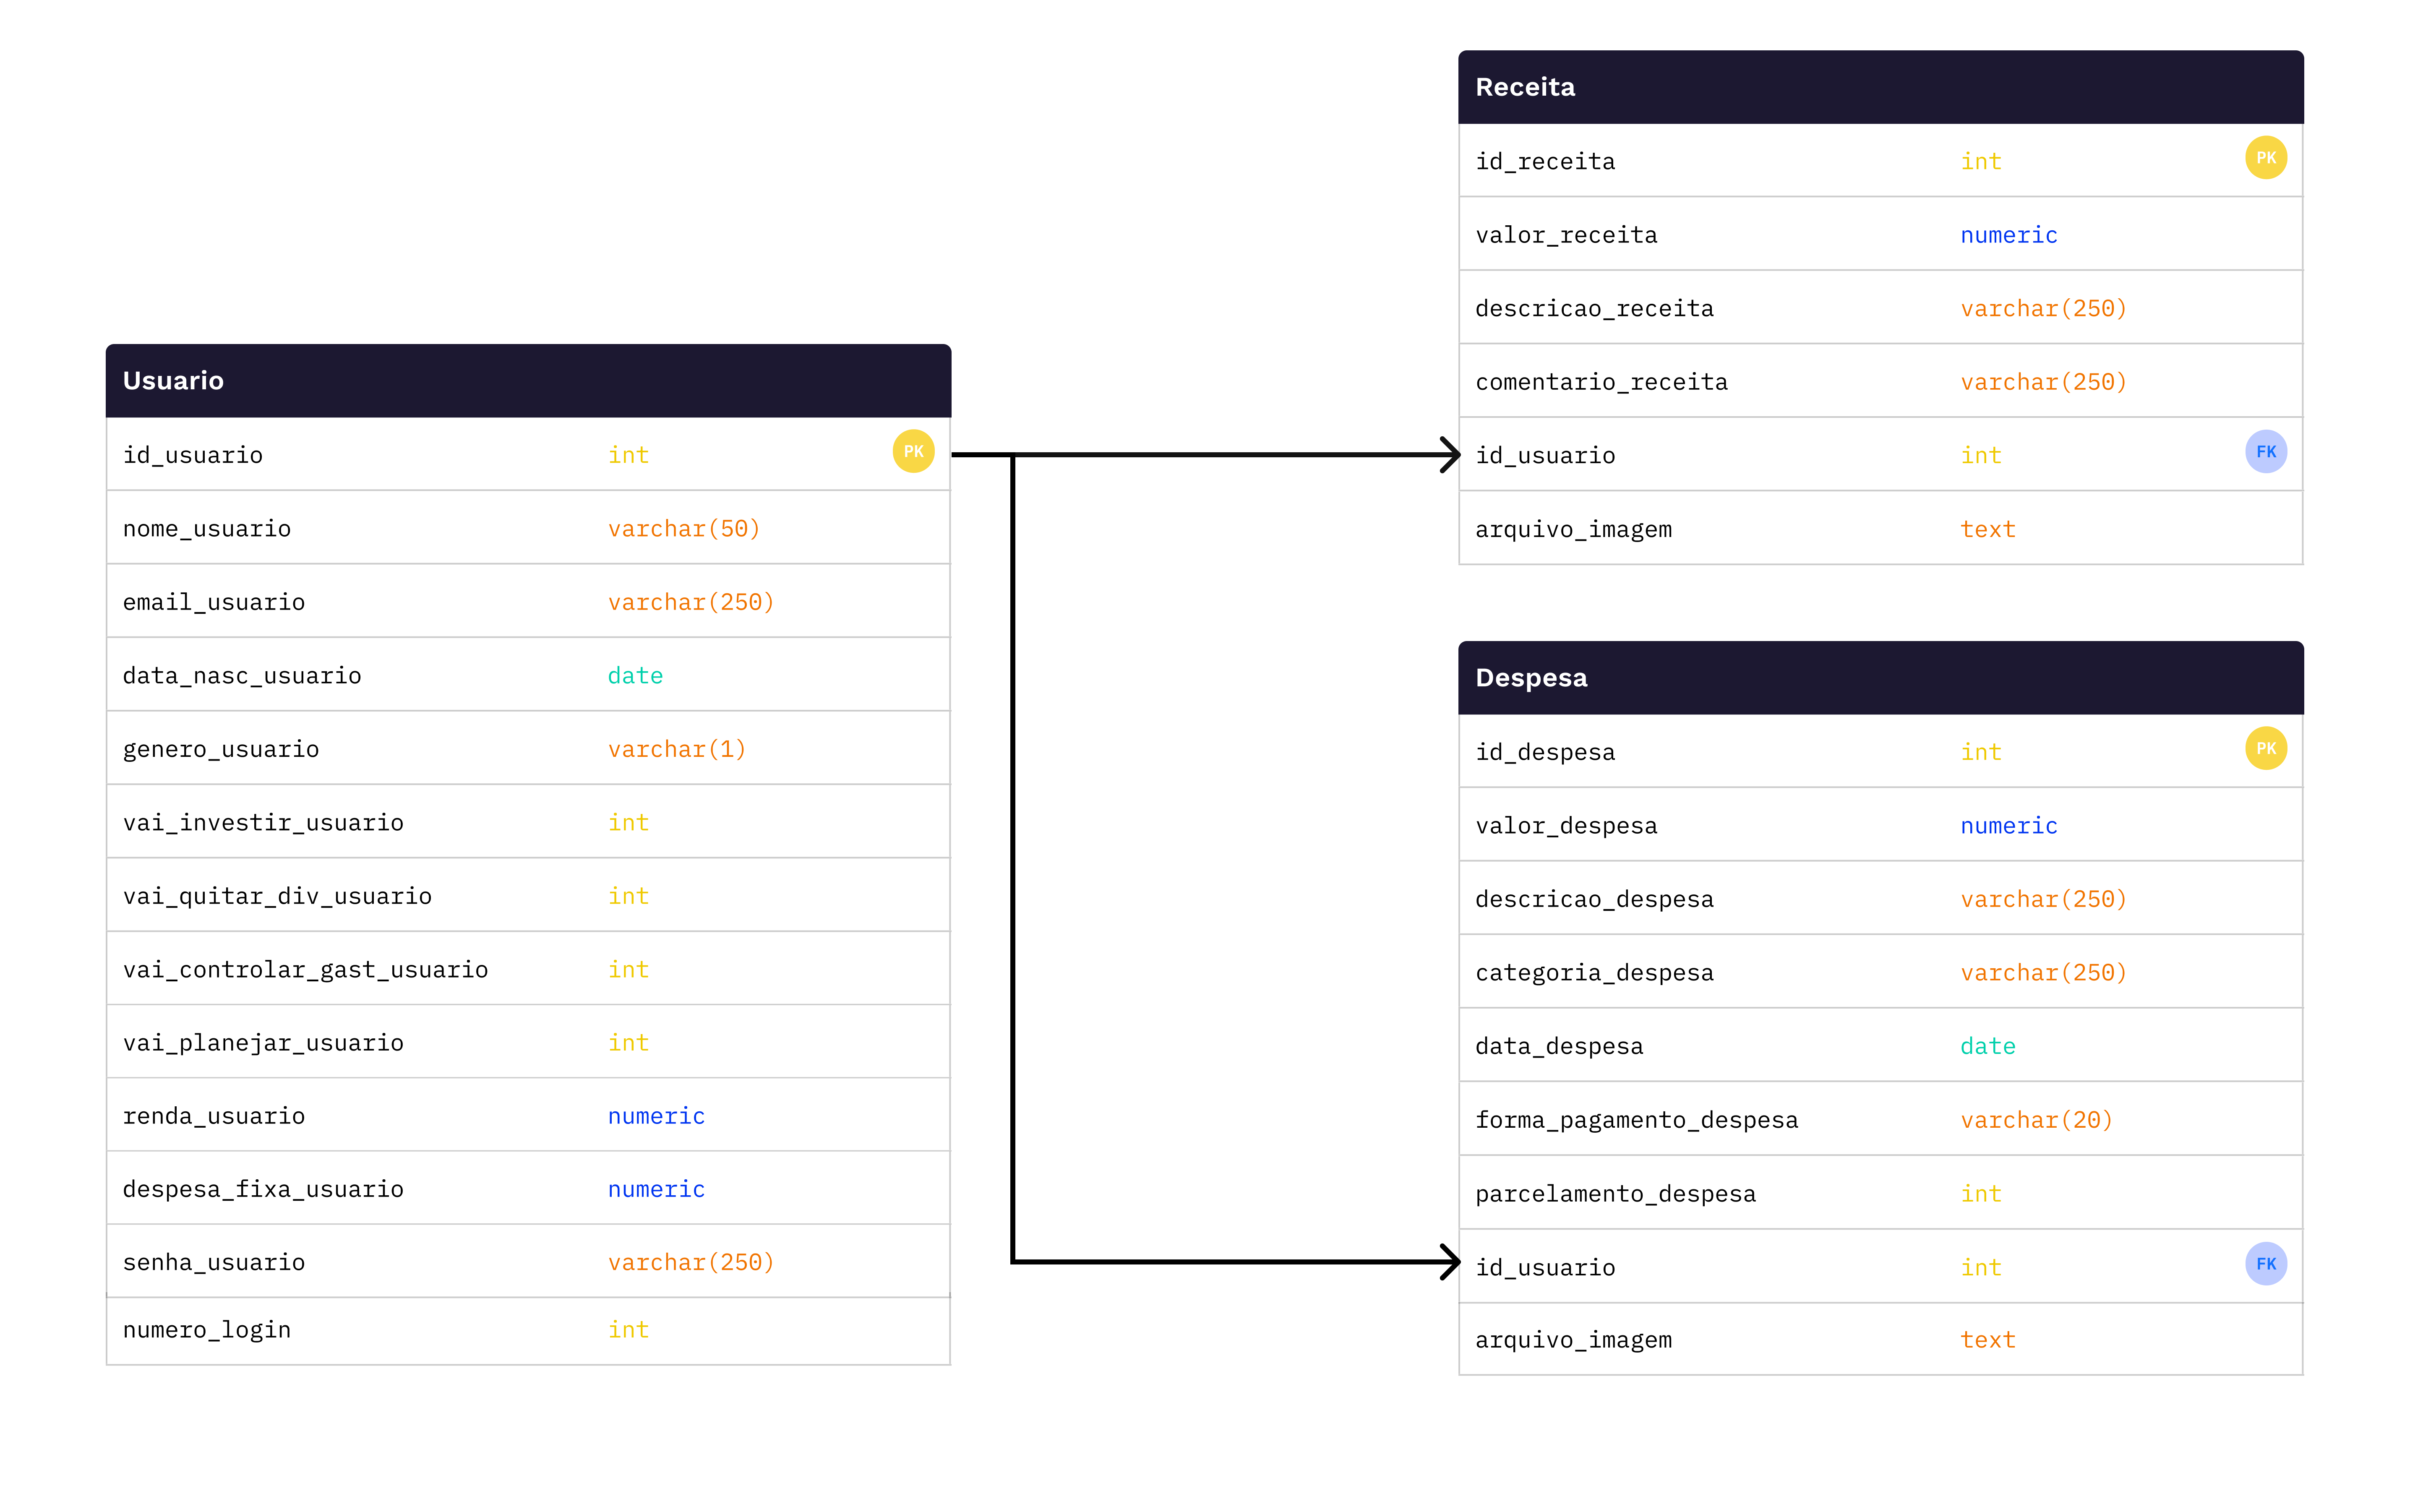
\includegraphics[scale=0.18]{figs/uml.png}
            \captionof{figure}{Desenho do Projeto do Banco de Dados}
            \label{fig:uml}
        \end{minipage}
    \end{center}

\section{Dicionário Básico do Banco de Dados}

    A tabela 1 corresponde ao dicionário da tabela 'usuario'.

\begin{table}[ht]
    \centering
    \setlength{\extrarowheight}{3pt}  % Aumenta a altura das linhas da tabela

    \begin{center}
        \begin{minipage}{\textwidth}
            \centering
            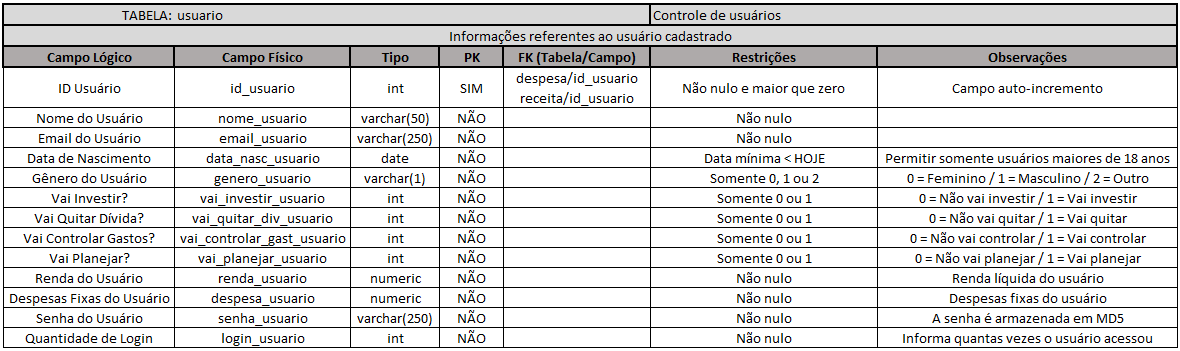
\includegraphics[scale=0.5]{figs/tab1.png}
        \end{minipage}
    \end{center}

    \caption{Dicionário da Tabela de Usuário}
    \label{tab:tab1}
\end{table}


    A tabela 2 corresponde ao dicionário da tabela 'despesa'.

\begin{table}[ht]
    \centering
    \setlength{\extrarowheight}{3pt}  % Aumenta a altura das linhas da tabela

    \begin{center}
        \begin{minipage}{\textwidth}
            \centering
            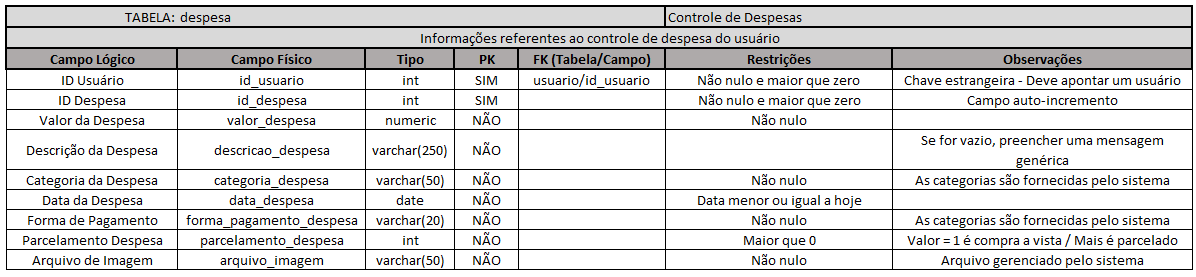
\includegraphics[scale=0.5]{figs/tab2.png}
        \end{minipage}
    \end{center}

    \caption{Dicionário da Tabela de Despesas}
    \label{tab:tab1}
\end{table}

    A tabela 3 corresponde ao dicionário da tabela 'receita'.

\begin{table}[ht]
    \centering
    \setlength{\extrarowheight}{3pt}  % Aumenta a altura das linhas da tabela

    \begin{center}
        \begin{minipage}{\textwidth}
            \centering
            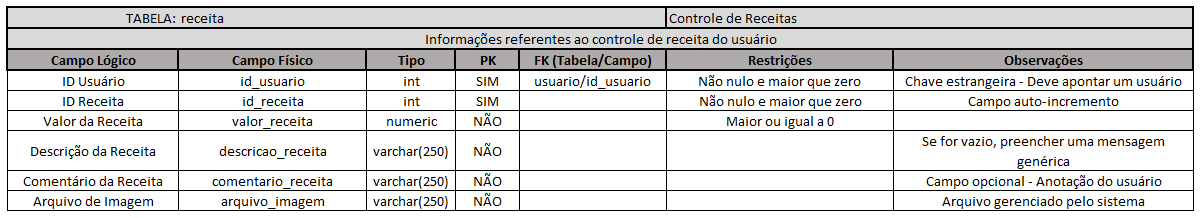
\includegraphics[scale=0.5]{figs/tab3.png}
        \end{minipage}
    \end{center}

    \caption{Dicionário da Tabela de Receitas}
    \label{tab:tab1}
\end{table}

\vspace{\baselineskip}
\vspace{\baselineskip}
\vspace{\baselineskip}

\section{Implementação}

Nesta seção do projeto serão apresentadas as principais telas desenvolvidas do \textit{Front End}.

\subsection{Tela de Login}

Esta é a tela inicial do aplicativo, onde todos os usuários poderão acessar utilizando um endereço de \textit{e-mail} e senha previamente cadastrados. Caso seja a primeira vez que o usuário está utilizando o aplicativo, será necessário realizar um cadastro clicando no botão \textbf{"Cadastrar"} conforme descrito na figura 15.

    \vspace{\baselineskip}
    \begin{center}
        \begin{minipage}{\textwidth}
            \centering
            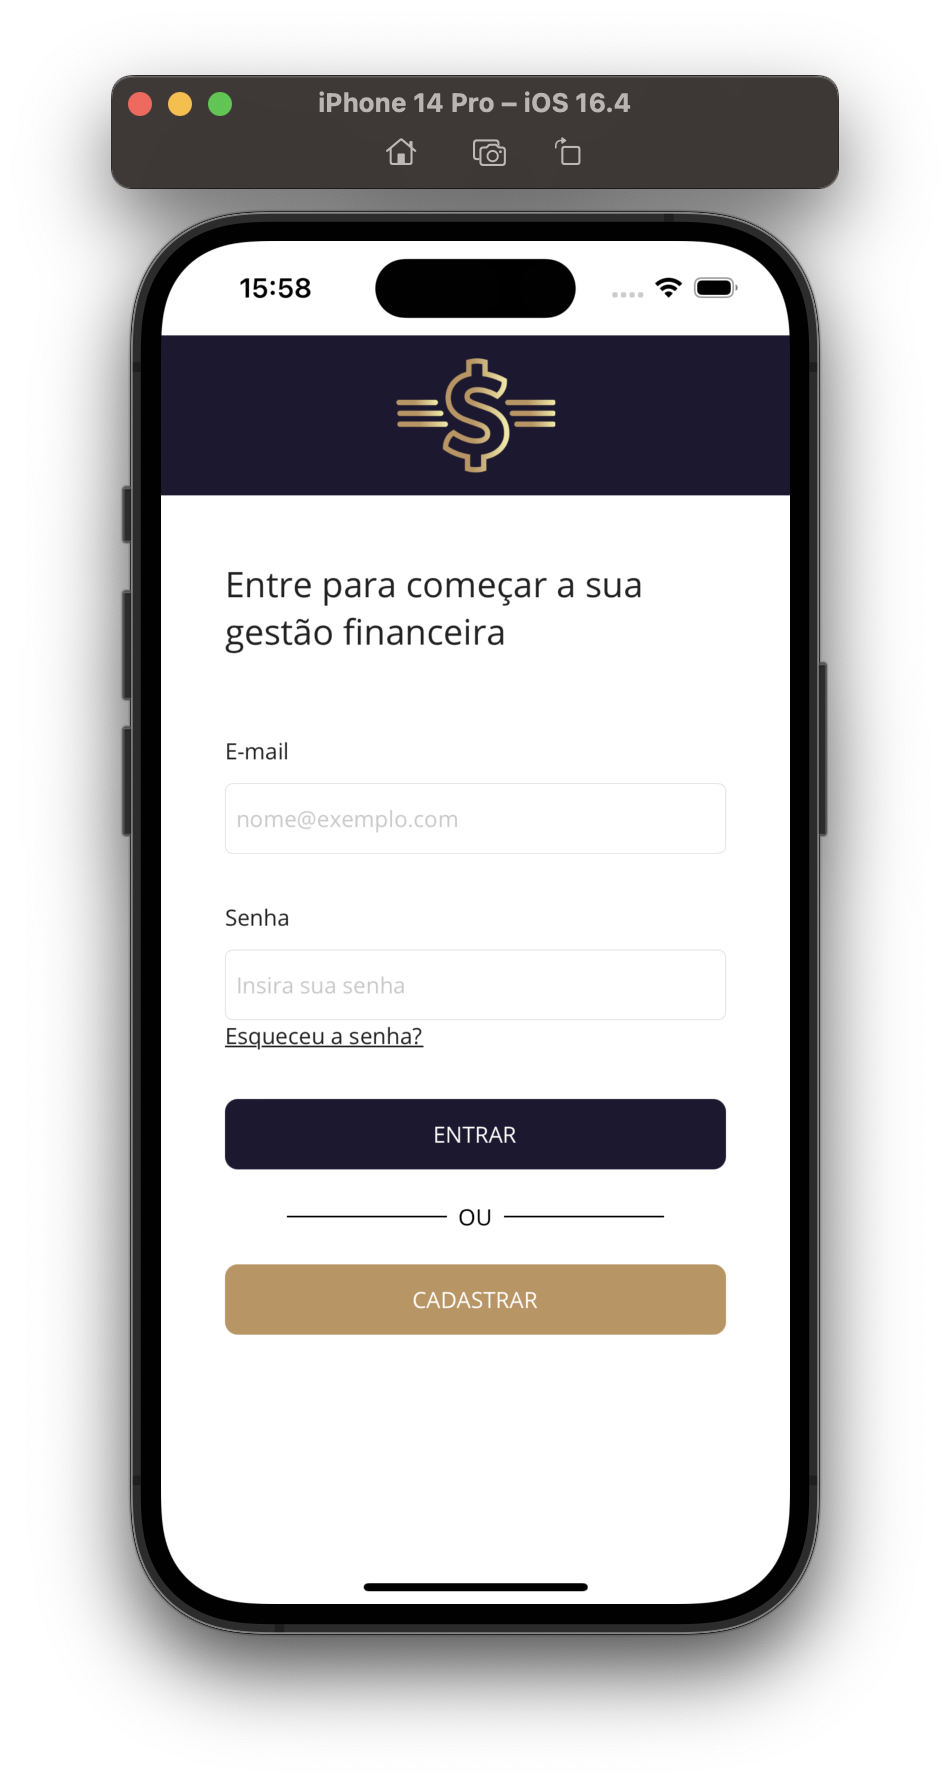
\includegraphics[scale=0.17]{figs/figura15.png}
            \captionof{figure}{Página de Login}
            \label{fig:uml}
        \end{minipage}
    \end{center}    

\subsection{Cadastro}

Conforme figura 16, para que o usuário possa realizar o cadastro, serão necessárias algumas informações, tais como: nome completo, \textit{e-mail}, data de nascimento e o gênero. Ao preencher todas as informações solicitadas, basta clicar no botão \textbf{“Próximo”}.

    \begin{center}
        \begin{minipage}{0.3\textwidth}
            \centering
            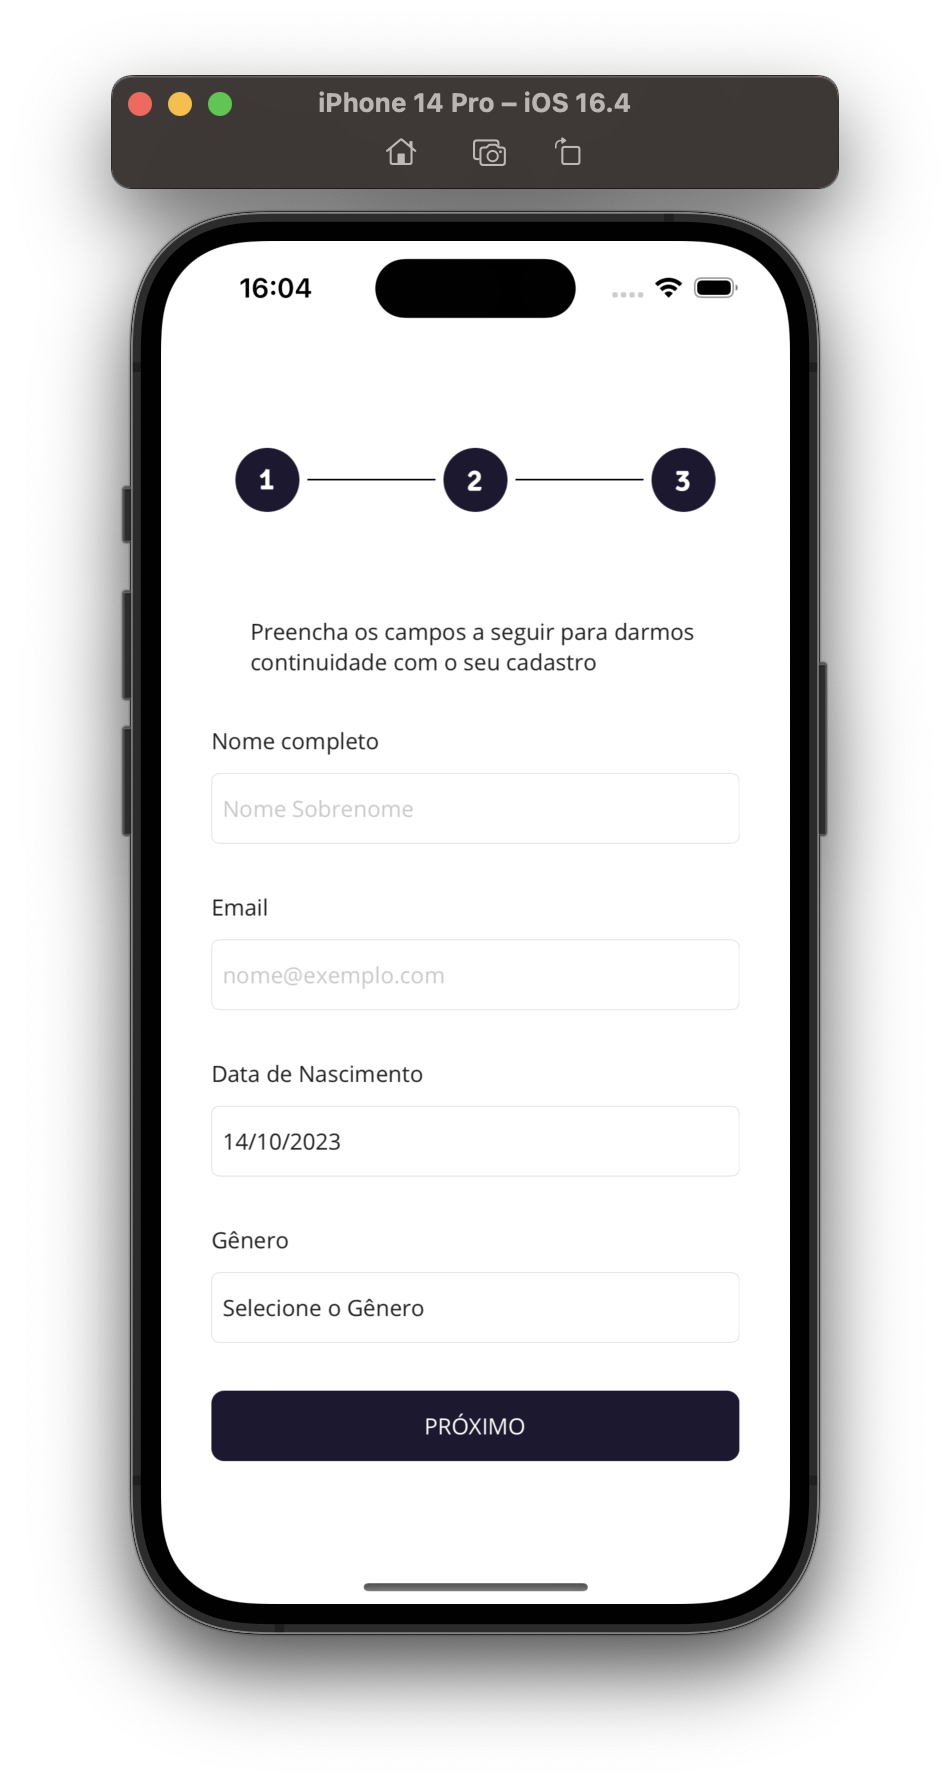
\includegraphics[scale=0.17]{figs/figura16.png}
            \captionof{figure}{Cadastro I}
            \label{fig:figura16}
        \end{minipage}%
    \end{center}
    

Conforme figura 17, uma nova tela aparecerá contendo alguns objetivos, bem como a média mensal de renda e despesas, a fim de entendermos melhor o perfil do usuário. Após preencher todos os campos obrigatórios, clique no botão \textbf{“Próximo”}.

    \begin{center}
        \begin{minipage}{0.3\textwidth}
            \centering
            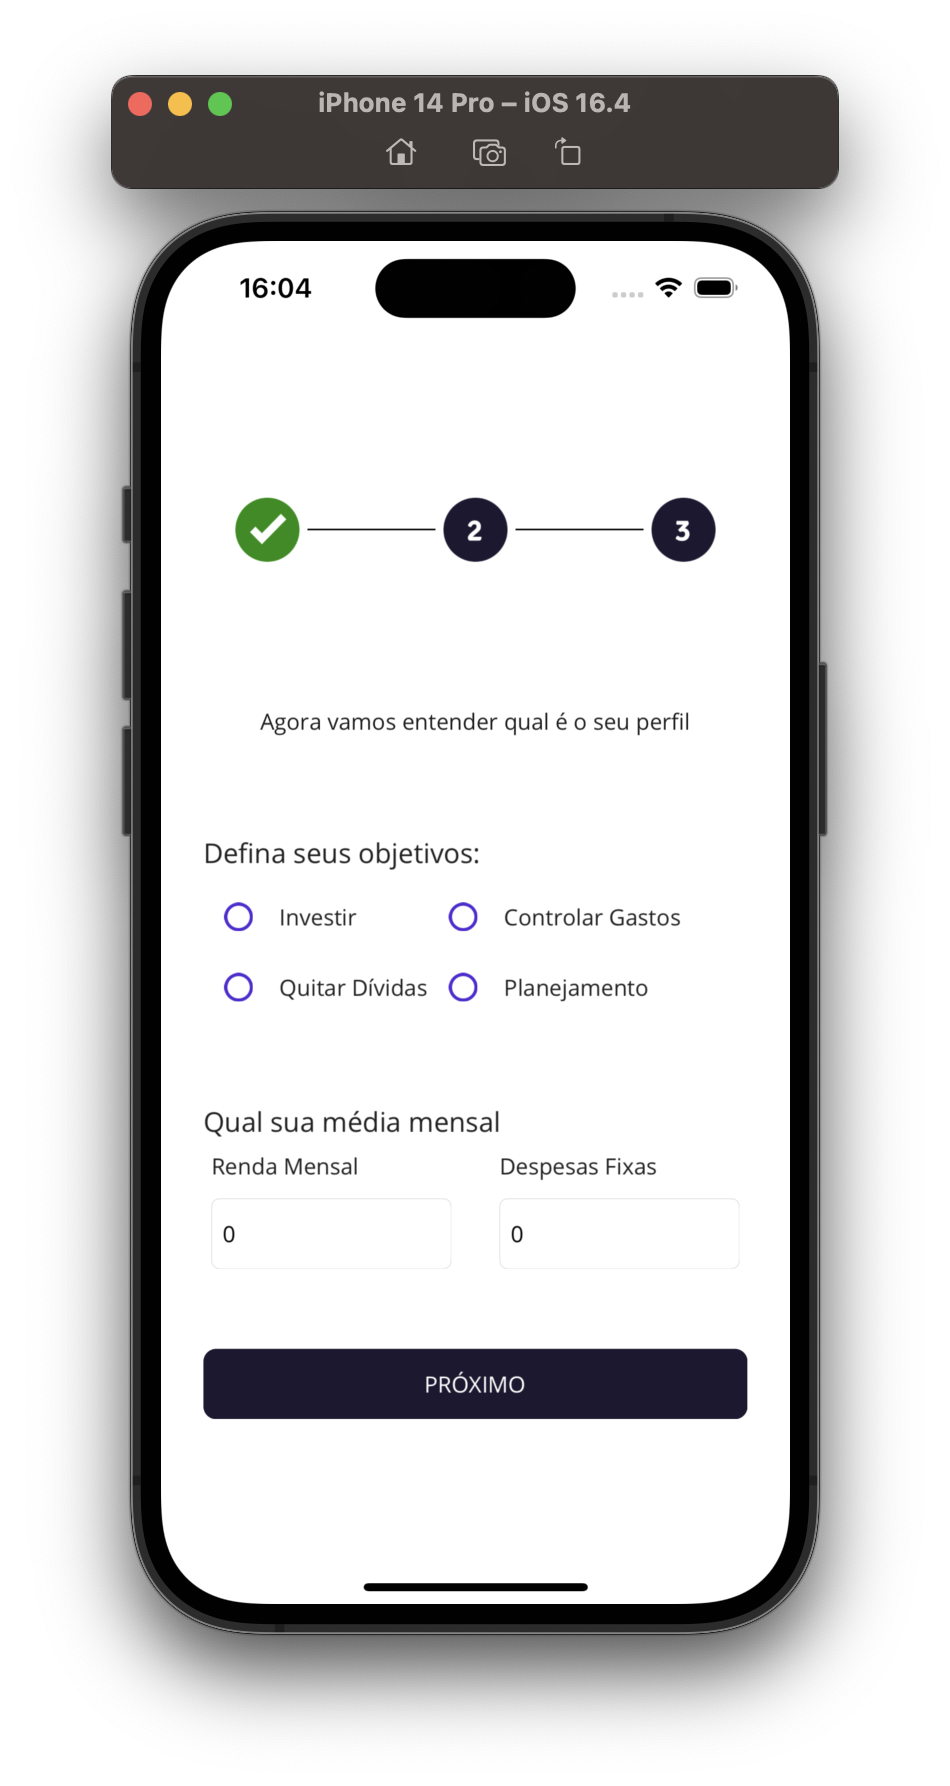
\includegraphics[scale=0.2]{figs/figura17.png}
            \captionof{figure}{Cadastro II}
            \label{fig:figura17}
        \end{minipage}%
    \end{center}

Conforme figura 18, aparecerá uma última tela destinada à criação de senha. Algumas especificações são de extrema importância para garantir a segurança dos dados do usuário. A senha deve conter no mínimo 8 caracteres, incluindo ao menos um número, uma letra maiúscula e uma letra minúscula. Repita a senha para verificar se digitou corretamente e, para finalizar, clique no botão \textbf{“Próximo”}. 

    \begin{center}
        \begin{minipage}{0.3\textwidth}
            \centering
            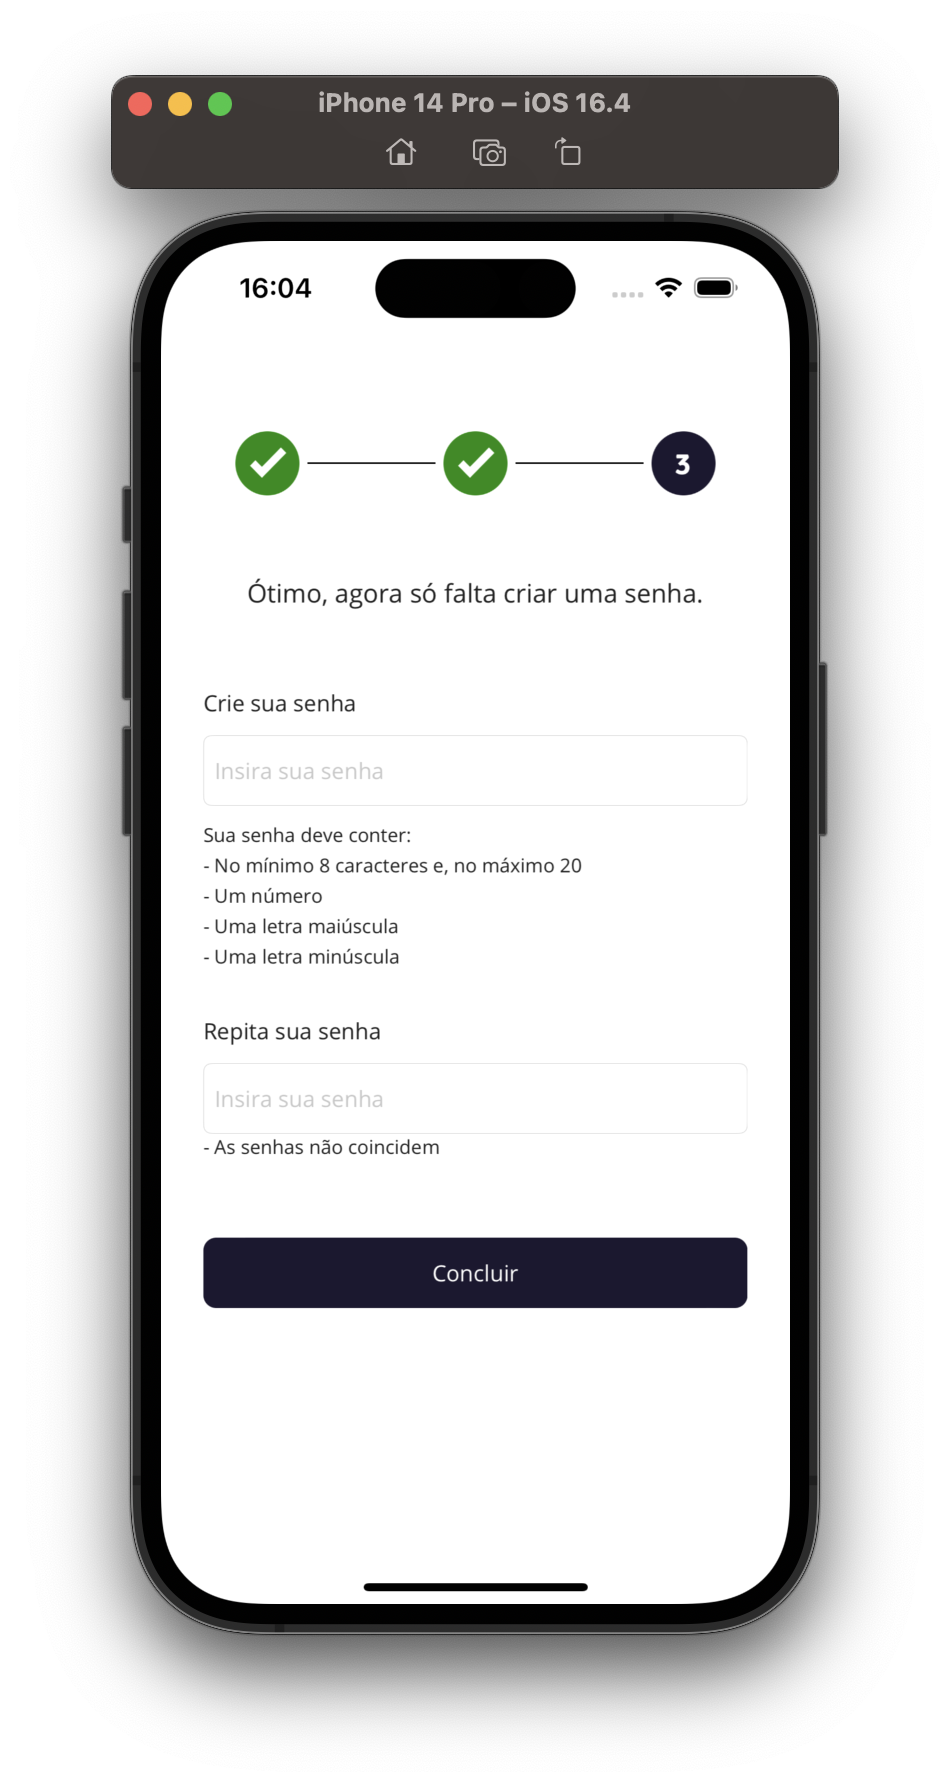
\includegraphics[scale=0.2]{figs/figura18.png}
            \captionof{figure}{Cadastro III}
            \label{fig:figura18}
        \end{minipage}%
    \end{center}

\vspace{\baselineskip}
\vspace{\baselineskip}
\vspace{\baselineskip}
\vspace{\baselineskip}
\vspace{\baselineskip}
\vspace{\baselineskip}

Na figura 19 apresentada, uma nova tela será exibida apenas para confirmar que o cadastro foi concluído com sucesso.

    \vspace{\baselineskip}
    \begin{center}
        \begin{minipage}{\textwidth}
            \centering
            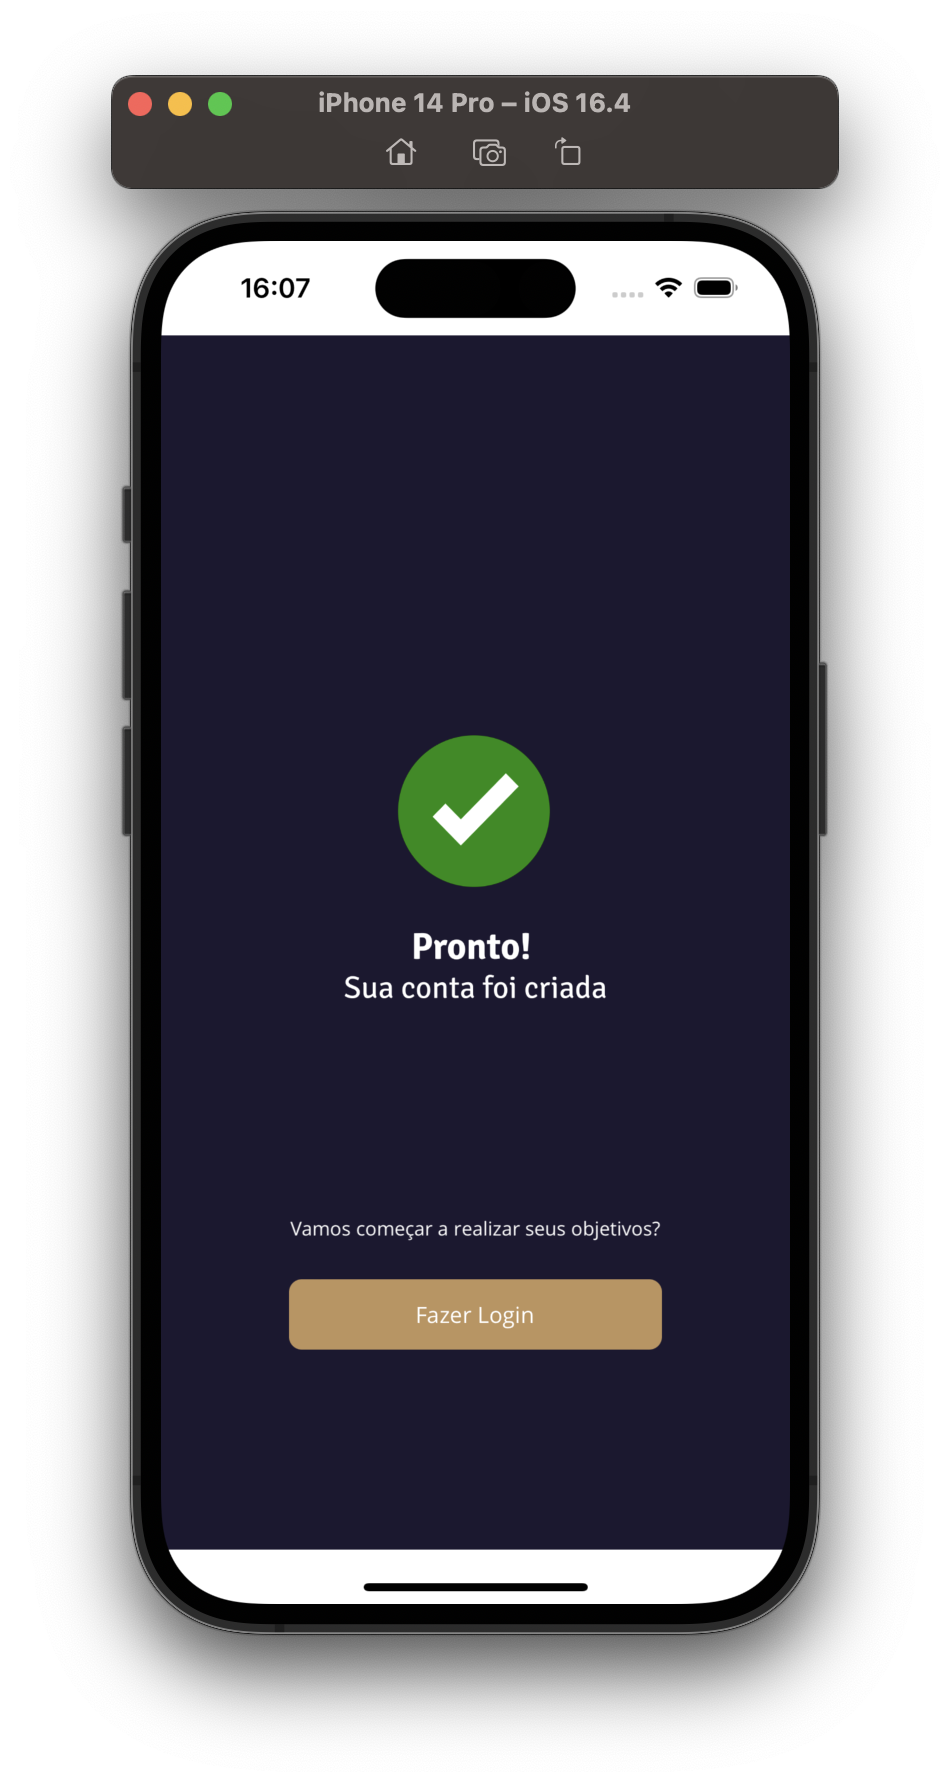
\includegraphics[scale=0.2]{figs/figura19.png}
            \captionof{figure}{Conta Criada}
            \label{fig:figura19}
        \end{minipage}
    \end{center}  
    
\subsection{Menu Principal}

Na figura 20 é descrito o menu principal

    \vspace{\baselineskip}
    \begin{center}
        \begin{minipage}{\textwidth}
            \centering
            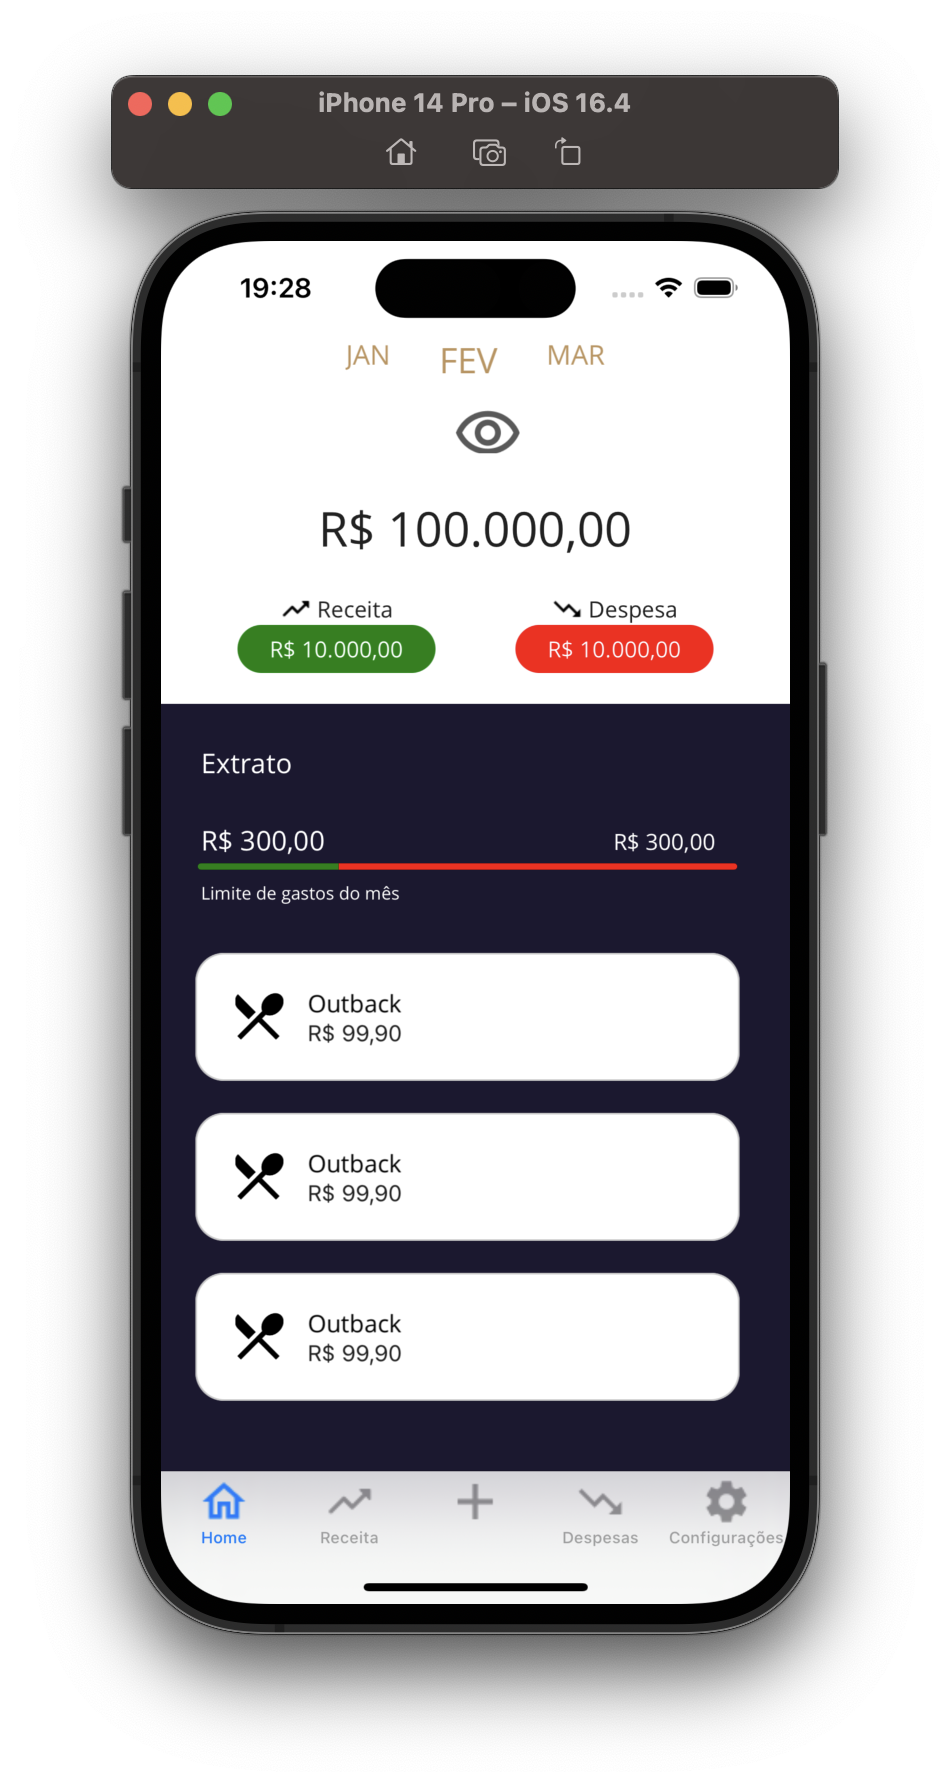
\includegraphics[scale=0.2]{figs/fig20.png}
            \captionof{figure}{Menu Principal}
            \label{fig:figura20}
        \end{minipage}
    \end{center}  

Após fazer o login, é possível utilizar o aplicativo, a imagem acima representa o menu principal, ou também bastante conhecida como \textit{“home”}, contendo diversas opções, tais como: saldo disponível, receita, despesas, extrato e alguns botões na parte inferior da tela. Além disso na parte superior da tela é possível ver informações referentes a meses passados e ou futuros. 

\subsection{Menu Principal com Informações Escondidas}

Na figura 21 é descrito o menu principal com informações escondidas.

    \vspace{\baselineskip}
    \begin{center}
        \begin{minipage}{\textwidth}
            \centering
            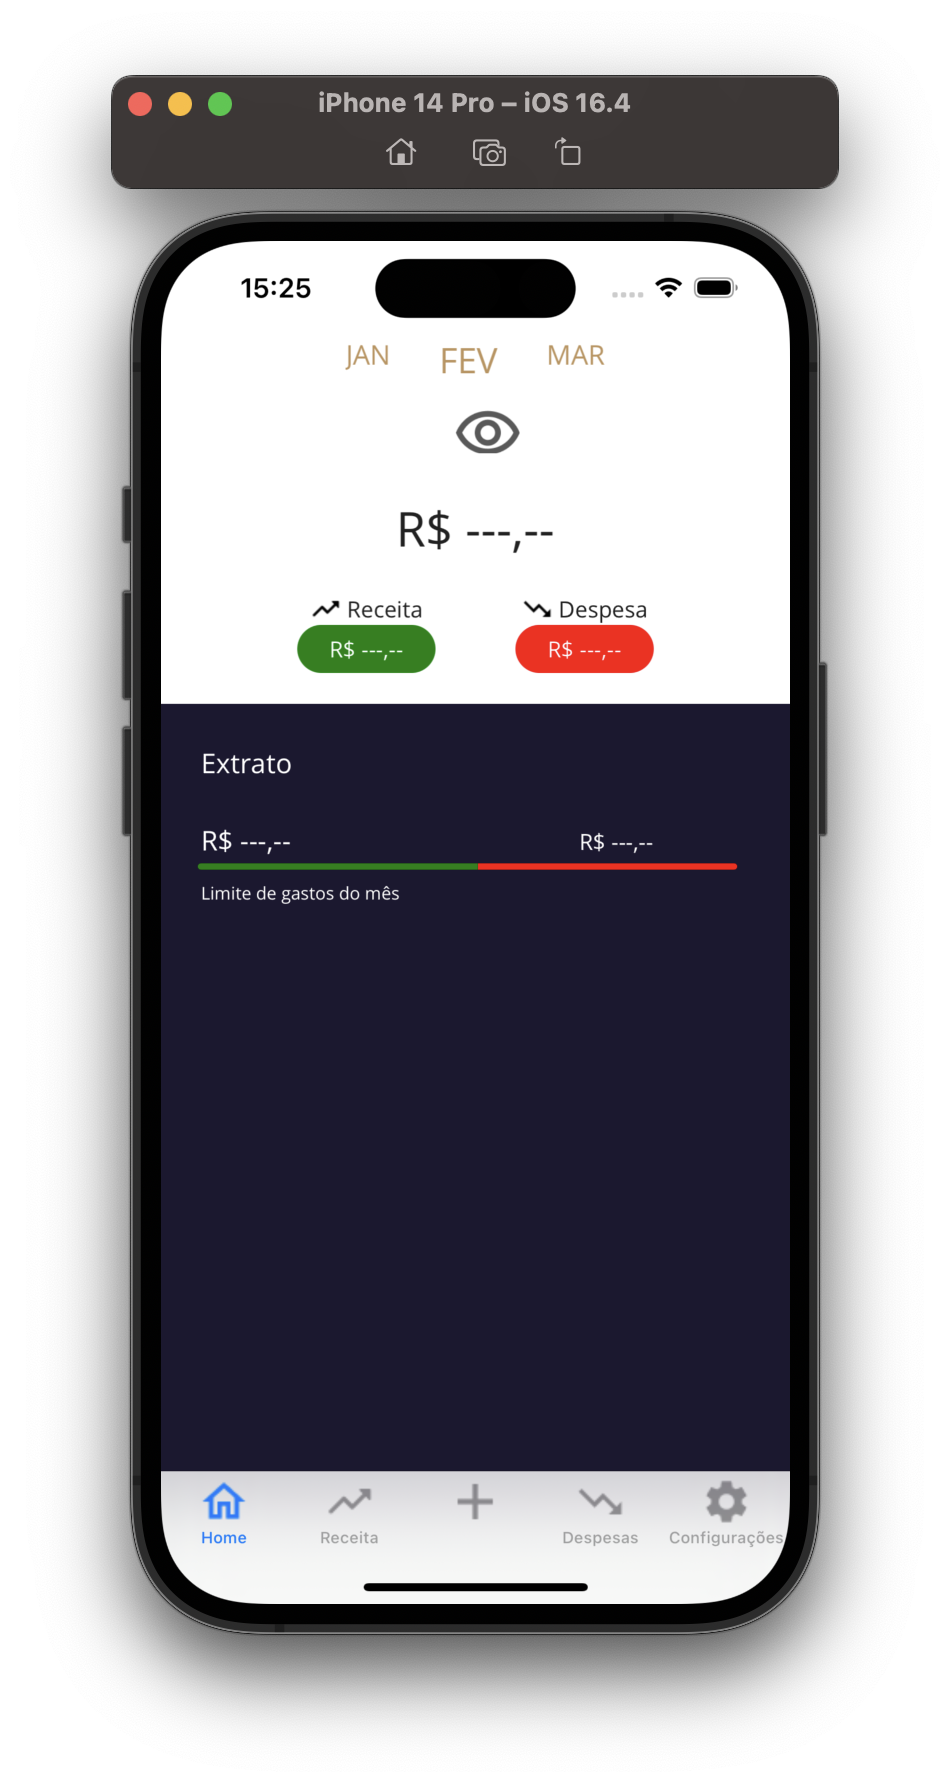
\includegraphics[scale=0.2]{figs/figura21.png}
            \captionof{figure}{Menu Principal com Informações Escondidas}
            \label{fig:figura21}
        \end{minipage}
    \end{center}  

Há a possibilidade de esconder informações que o usuário não queira exibir, como o saldo, o valor do extrato, a receita e as despesas. Essas informações são apresentadas na figura 22.

    \vspace{\baselineskip}
    \begin{center}
        \begin{minipage}{\textwidth}
            \centering
            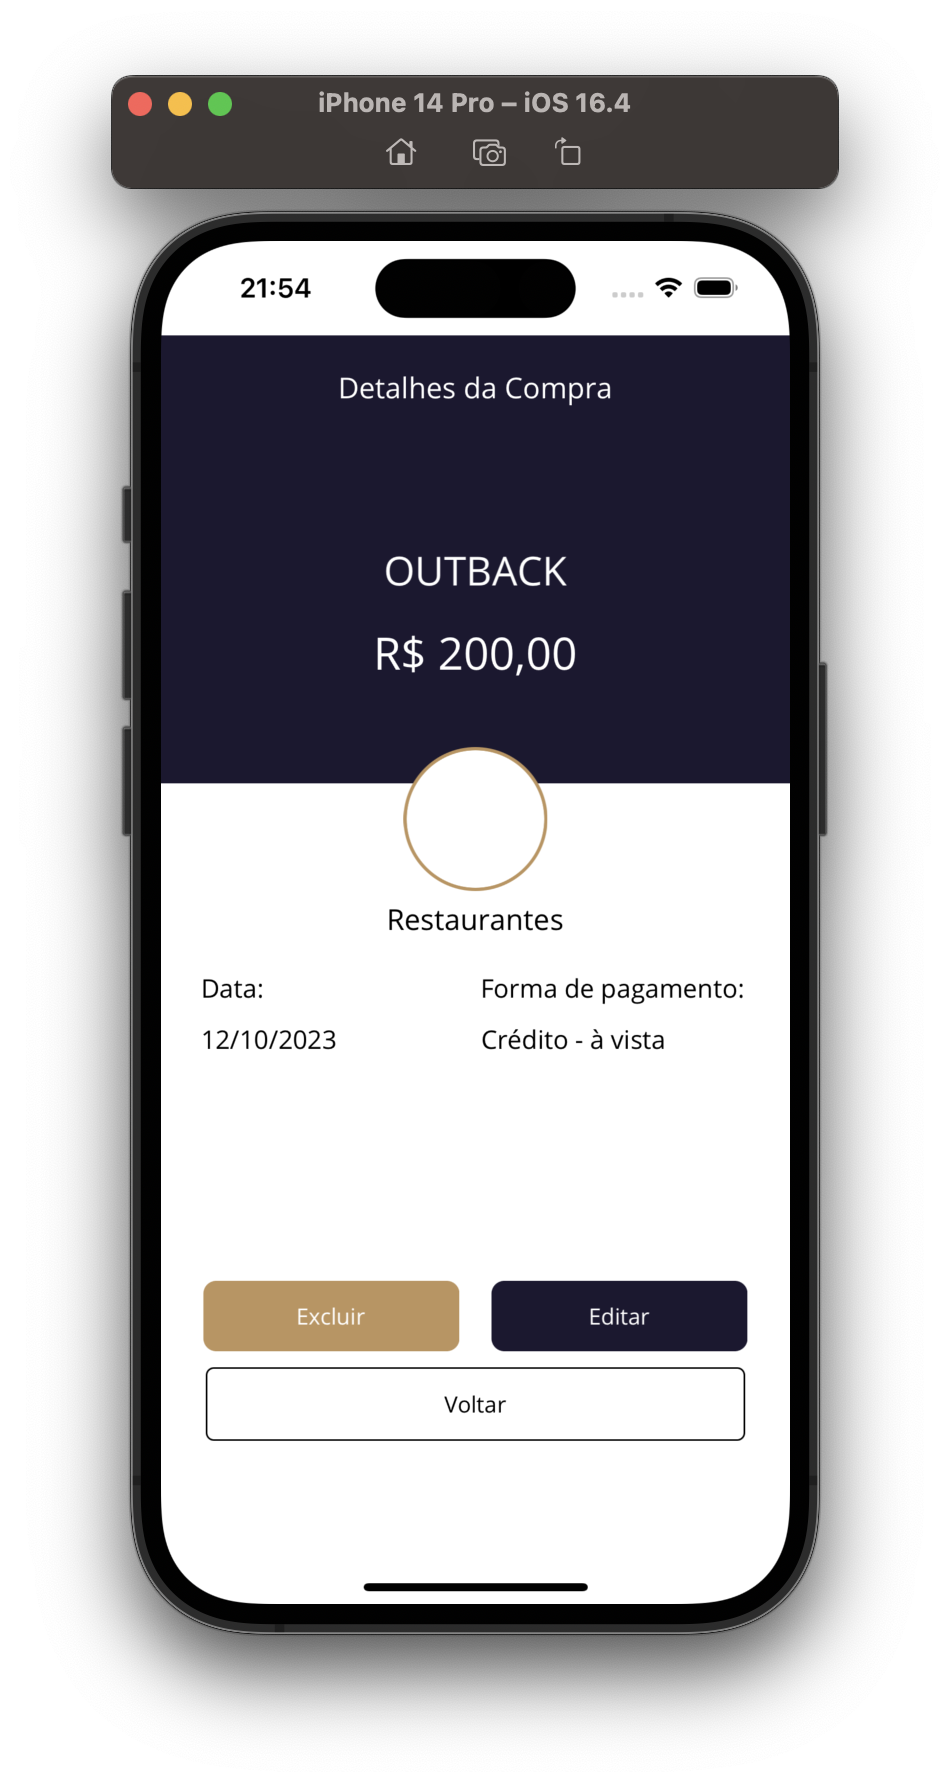
\includegraphics[scale=0.2]{figs/fig22.png}
            \captionof{figure}{Extrato com Informações}
            \label{fig:figura22}
        \end{minipage}
    \end{center}  

No extrato será possível visualizar um gasto detalhadamente, incluindo a data e hora da compra, numeração final do cartão utilizado e a opção de relatar uma compra que o cliente considerar não ter sido feita por ele. 

Conforme a figura 23, é possível notar que temos três opções clicando nesse botão central de \textbf{“+”}, onde, cada uma dessas opções significa uma funcionalidade diferente. A primeira opção é \textbf{“Importar PDF”} que será explicado logo abaixo. A segunda e a terceira opção são voltadas a adicionar algo que seria receita e despesa respectivamente. 

    \vspace{\baselineskip}
    \begin{center}
        \begin{minipage}{\textwidth}
            \centering
            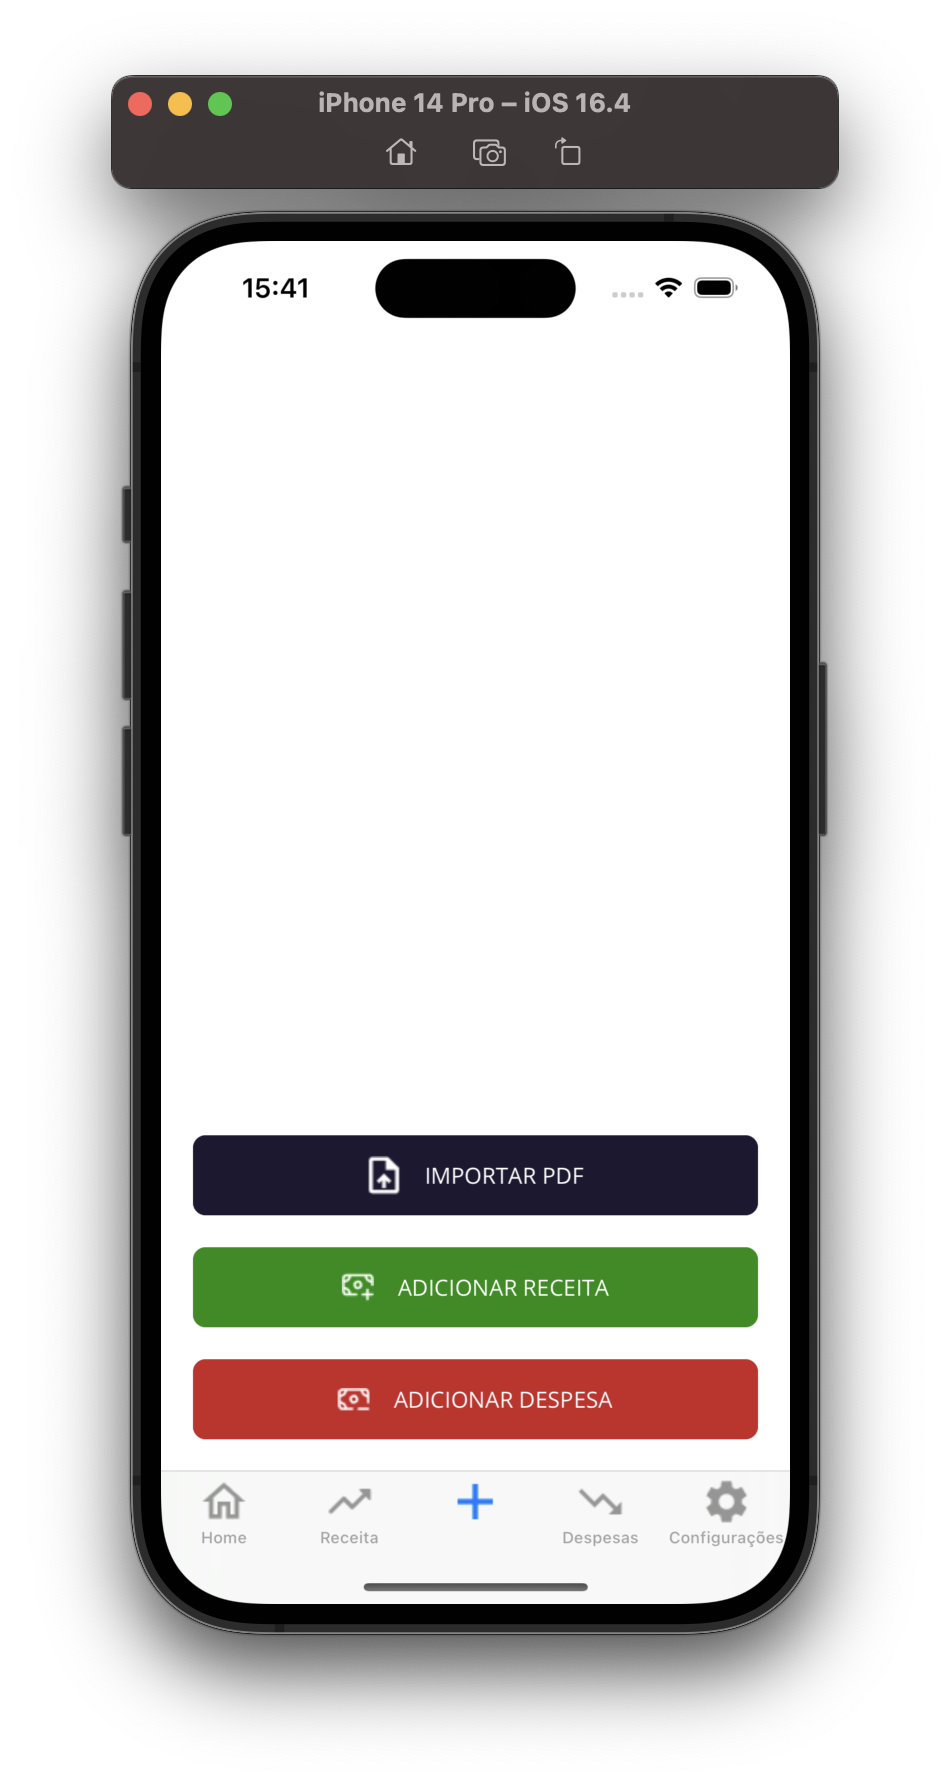
\includegraphics[scale=0.2]{figs/figura23.png}
            \captionof{figure}{Menu com Três Opções}
            \label{fig:figura23}
        \end{minipage}
    \end{center}     

Ao clicar na opção de \textbf{“Importar PDF”} uma nova tela para a importação de PDF aparecerá, assim como mostrado na figura 24. Nessa aba de importação de PDF, temos como campos a escolha do PDF a ser importado. Caso seja necessária uma senha para acessar o arquivo, basta clicar no botão \textbf{“Sim”} e imediatamente abaixo, o campo para digitar a senha será habilitado. Se não for necessária uma senha, selecione o botão \textbf{“Não”} que o campo abaixo permanecerá desativado. Ao finalizar clicar no botão \textbf{“Importar Arquivo”}, após clicar uma nova tela aparecerá indicando sucesso na operação, conforme figura 25. 

    \vspace{\baselineskip}
    \begin{center}
        \begin{minipage}{0.4\textwidth}
            \centering
            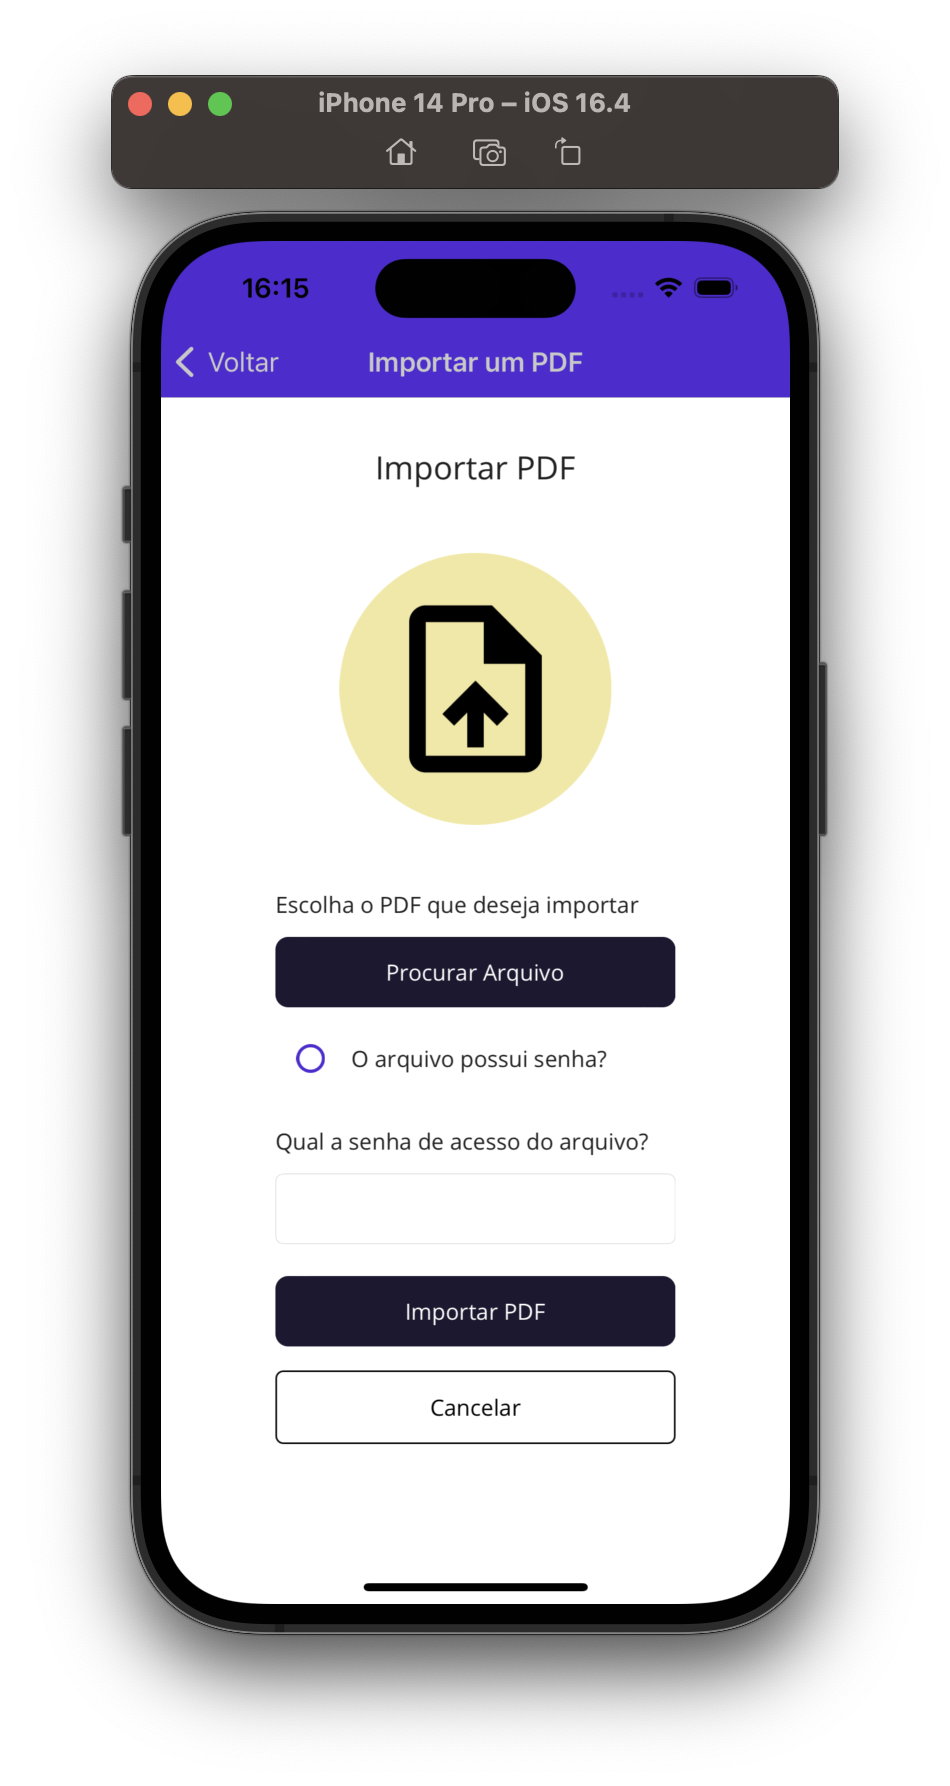
\includegraphics[scale=0.2]{figs/figura24.png}
            \captionof{figure}{Importar PDF I}
            \label{fig:figura24}
        \end{minipage}%
        \begin{minipage}{0.4\textwidth}
            \centering
            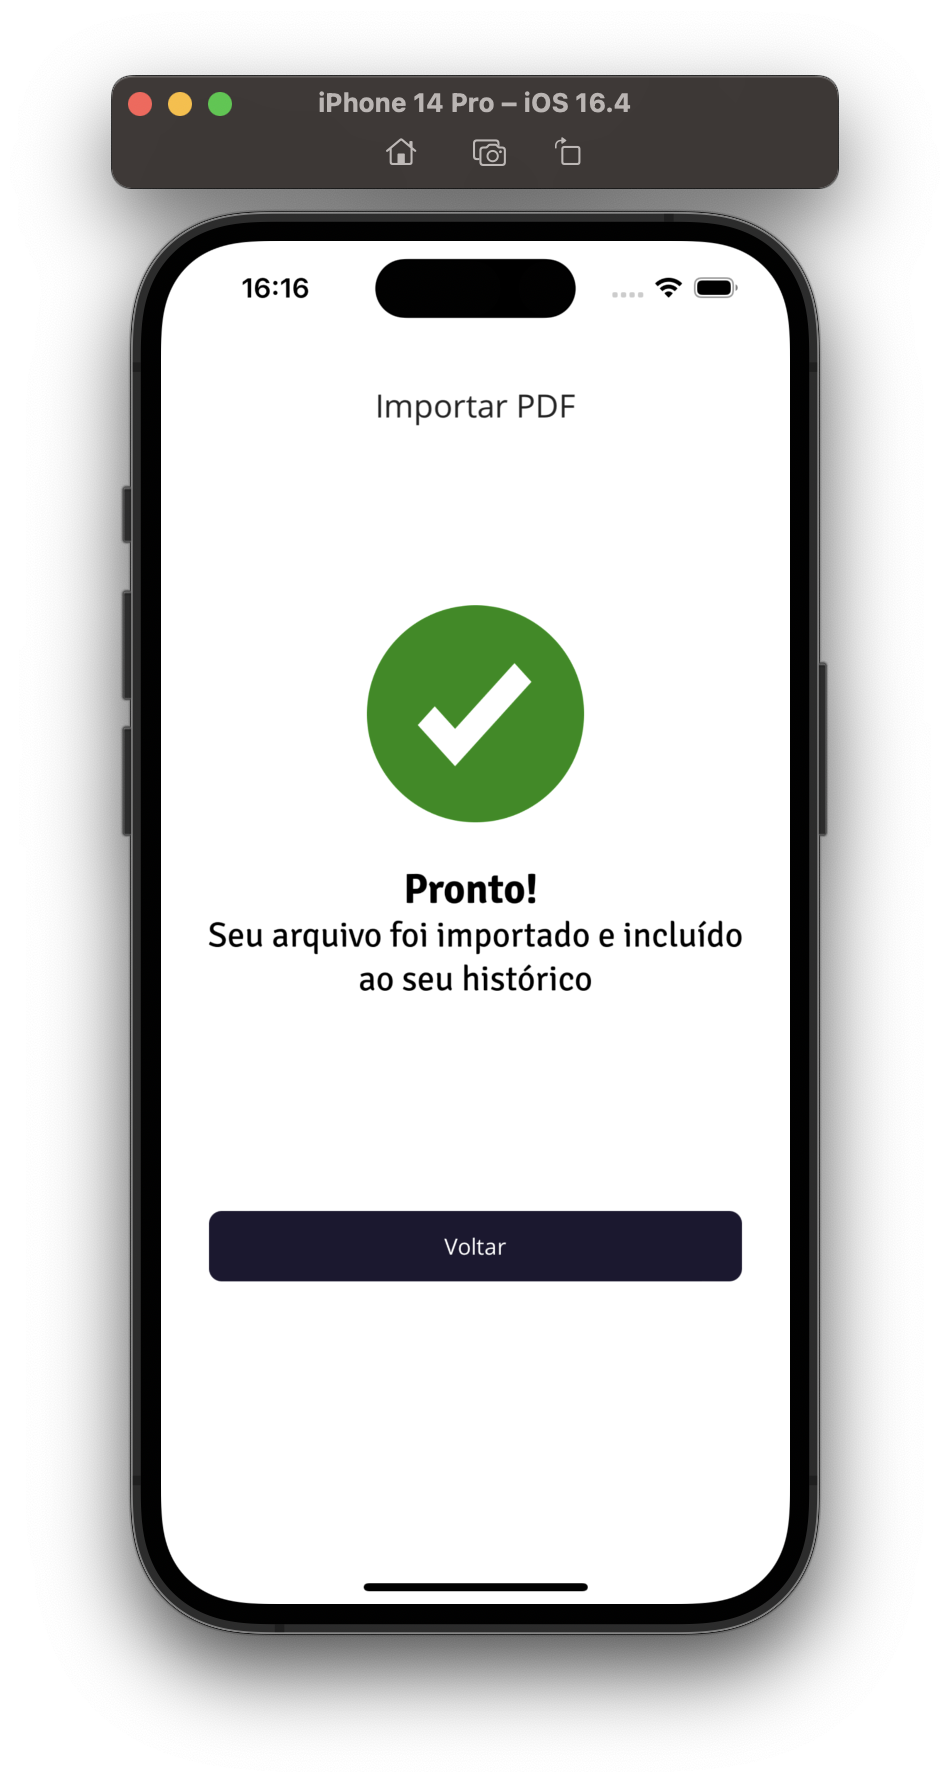
\includegraphics[scale=0.2]{figs/figura25.png}
            \captionof{figure}{Importar PDF II}
            \label{fig:figura25}
        \end{minipage}%
    \end{center}

A partir do Menu Principal ao clicar na opção \textbf{“Adicionar Receita”} aparecerá uma tela descrita na Figura 26. Nessa nova tela contém dois campos um obrigatório no qual um valor deve ser inserido, valor referente a receita. E um outro tópico não obrigatório que seria para adicionar uma descrição para essa receita. Ao preencher os devidos campos clique no botão \textbf{“Adicionar”}, e então uma tela apontando sucesso na operação aparecerá, conforme descrito na Figura 27. 

    \vspace{\baselineskip}
    \begin{center}
        \begin{minipage}{0.4\textwidth}
            \centering
            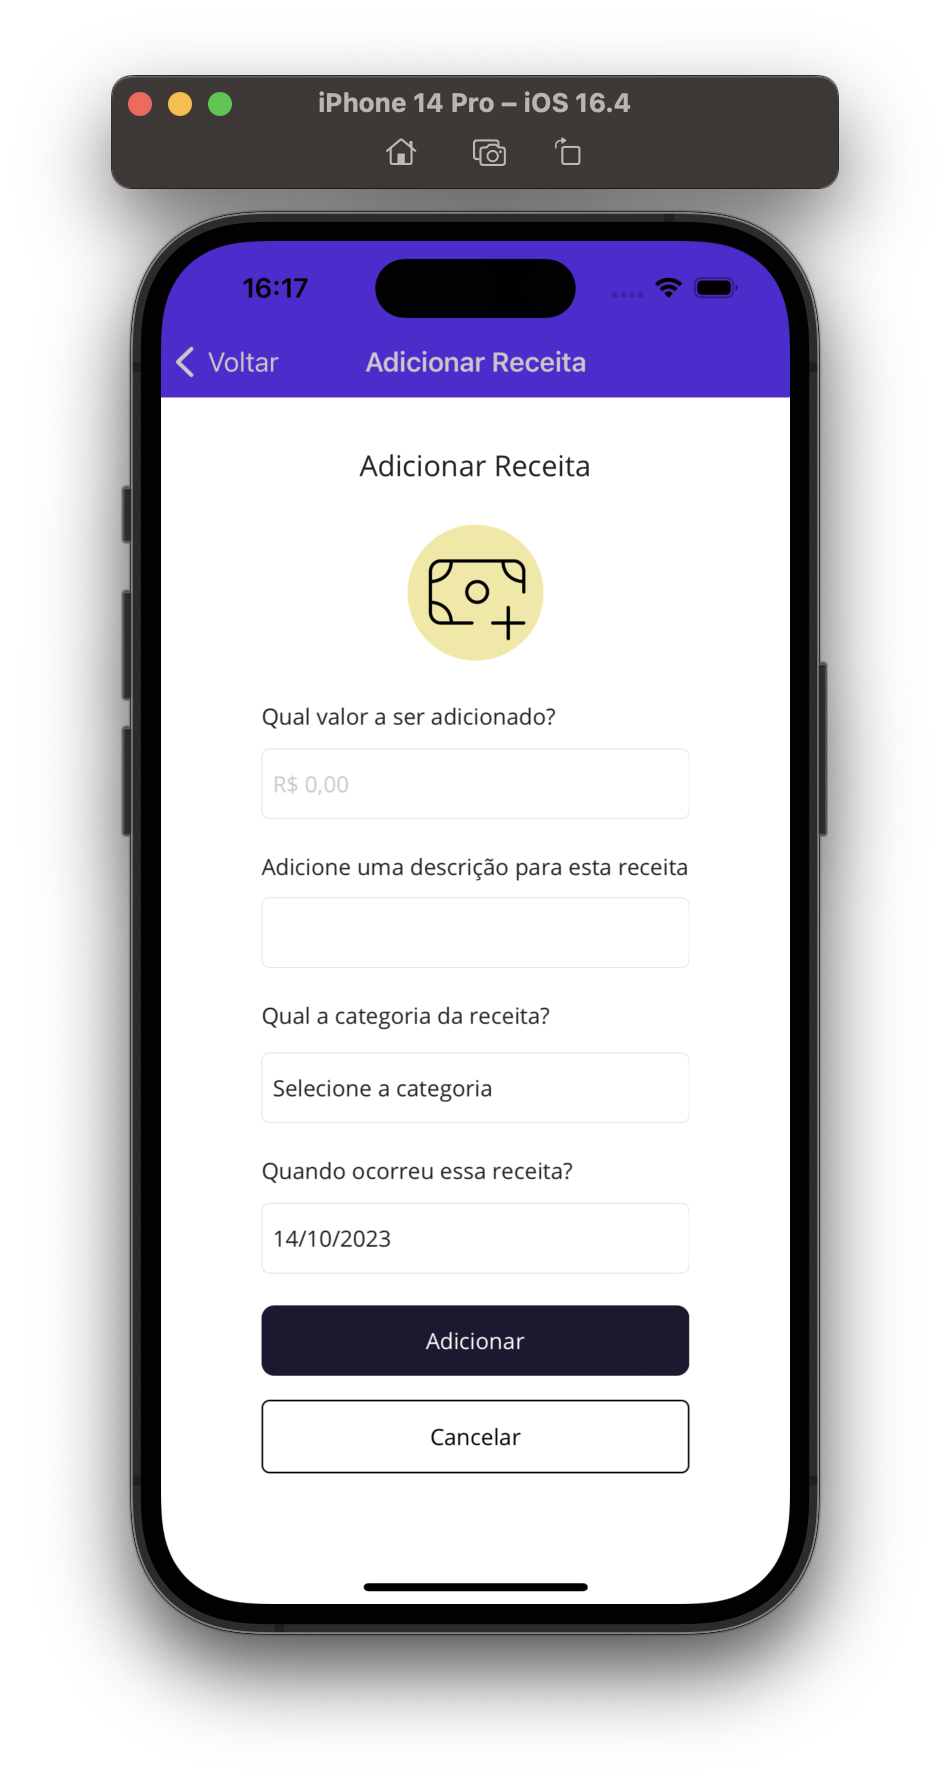
\includegraphics[scale=0.15]{figs/figura26.png}
            \captionof{figure}{Criar Receita I}
            \label{fig:figura26}
        \end{minipage}%
        \begin{minipage}{0.4\textwidth}
            \centering
            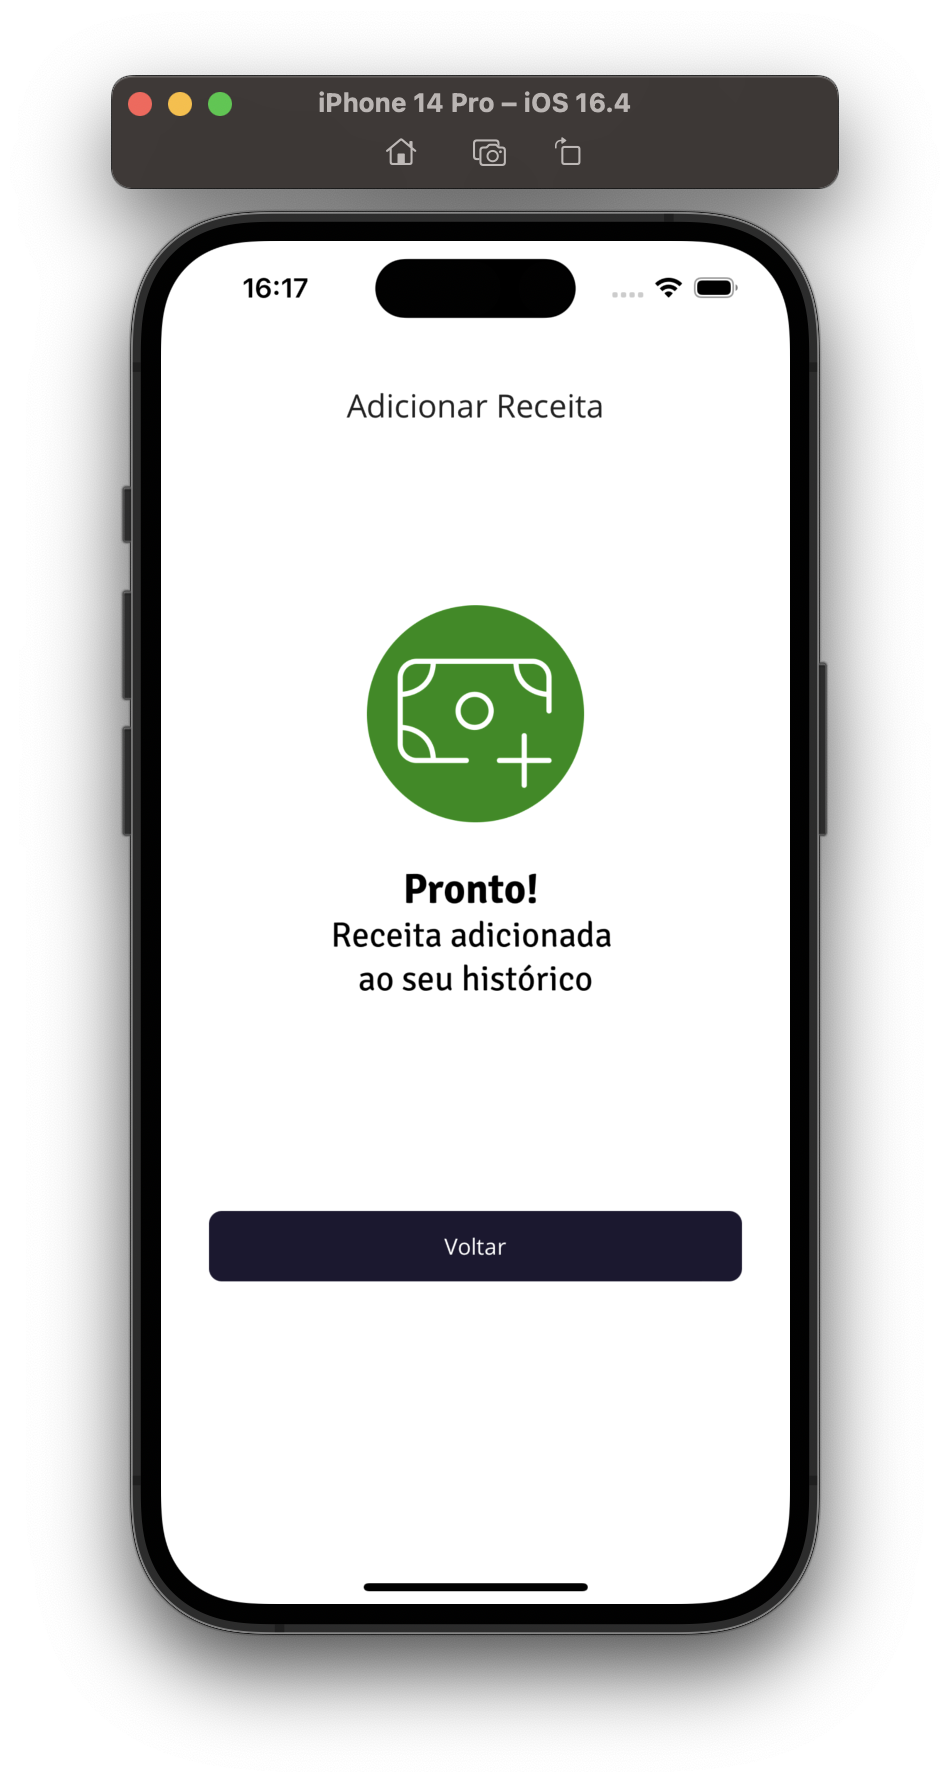
\includegraphics[scale=0.15]{figs/figura27.png}
            \captionof{figure}{Criar Receita II}
            \label{fig:figura27}
        \end{minipage}%
    \end{center}

De acordo com o Menu Principal, ao escolher a opção \textbf{“Adicionar Despesa”} aparecerá a tela da figura 28, contendo dois campos um obrigatório para colocar o valor da despesa, e um campo abaixo que não é obrigatório, para colocar uma descrição sobre a despesa. Ao preencher os campos, basta clicar no botão \textbf{“Adicionar”}. Uma nova tela contendo sucesso na despesa adicionada virá à tona, conforme figura 29.

    \vspace{\baselineskip}
    \begin{center}
        \begin{minipage}{0.4\textwidth}
            \centering
            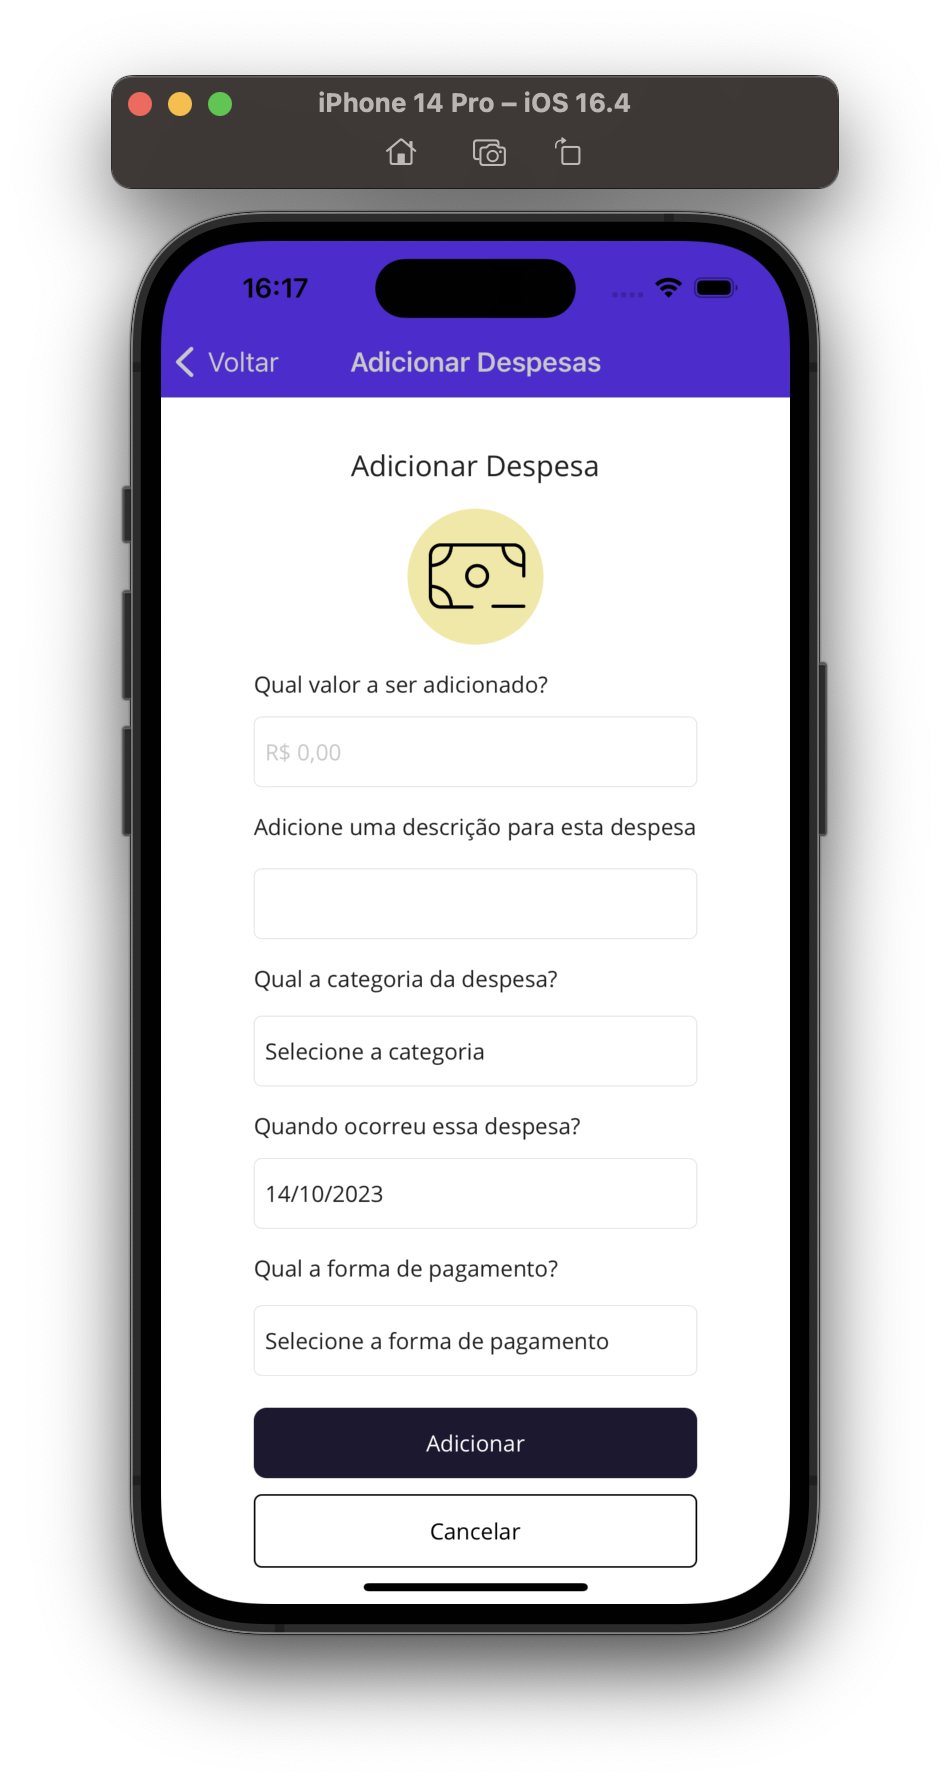
\includegraphics[scale=0.2]{figs/figura28.png}
            \captionof{figure}{Criar Despesa I}
            \label{fig:figura28}
        \end{minipage}%
        \begin{minipage}{0.4\textwidth}
            \centering
            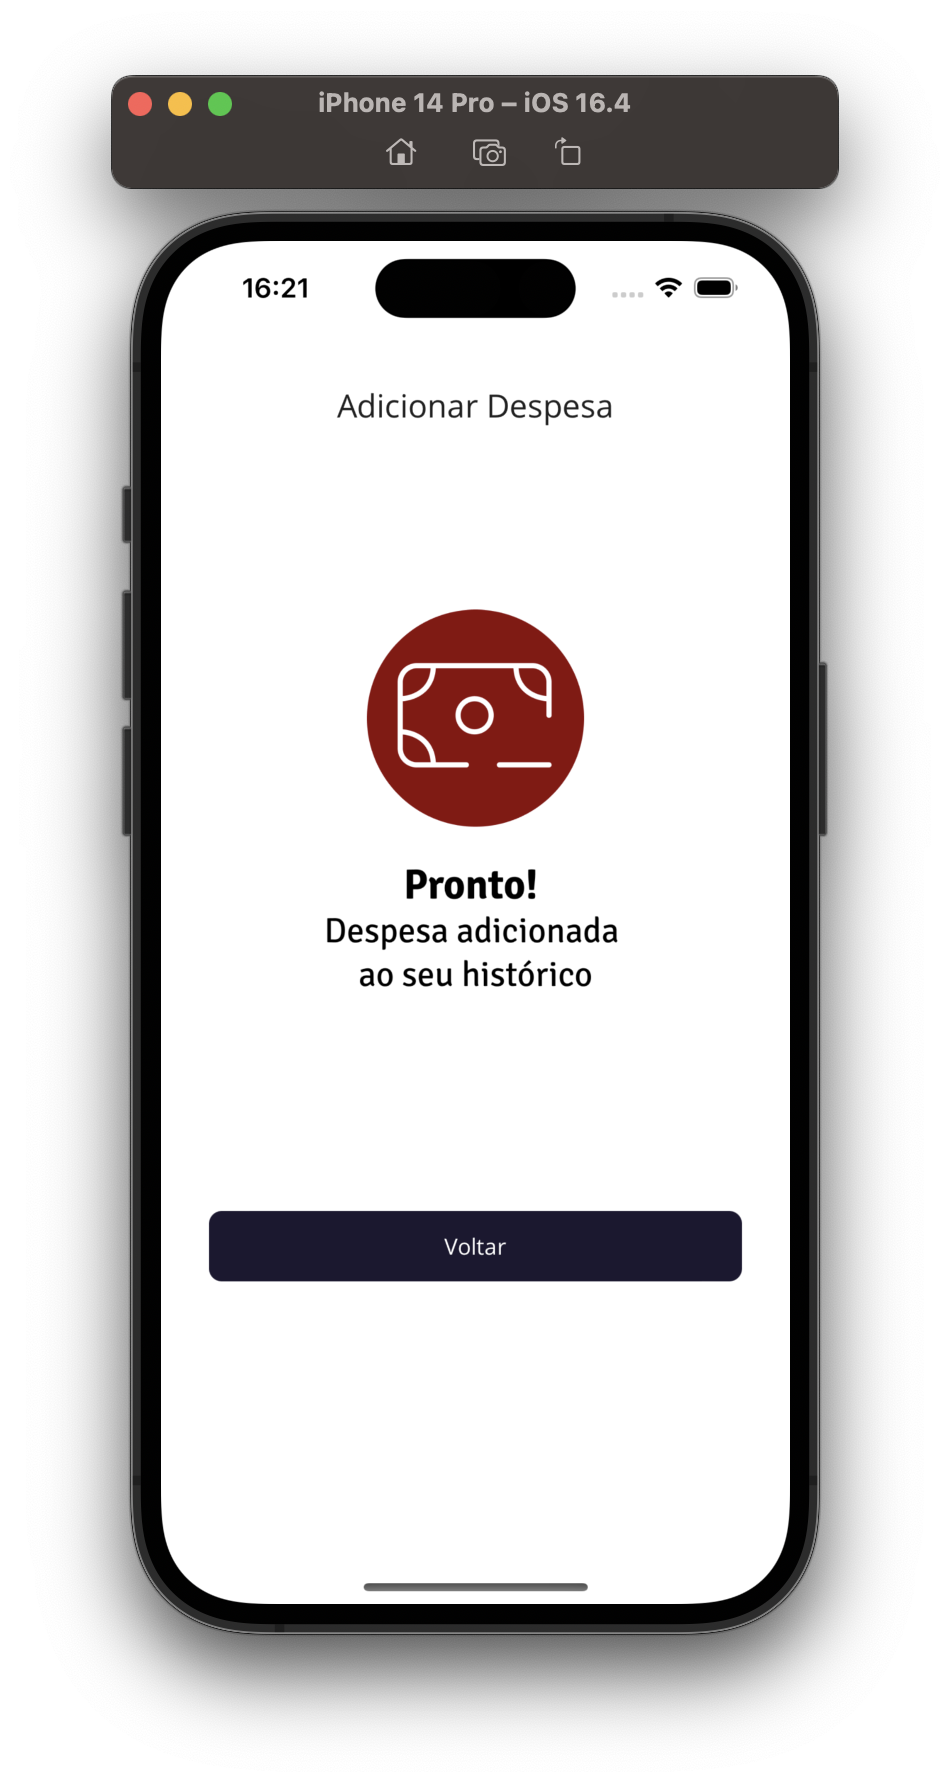
\includegraphics[scale=0.2]{figs/figura29.png}
            \captionof{figure}{Criar Despesa II}
            \label{fig:figura29}
        \end{minipage}%
    \end{center}
    
\subsection{Redefinição de Senha}

Caso o usuário esqueça a senha é possível redefini-la na tela de login clicando no botão \textbf{“Esqueci a Senha”}. Ao fazer isso, aparecerá a primeira tela acima, que contém um campo para inserir o \textit{e-mail} que terá a senha alterada, após inserir o \textit{e-mail} clique no botão \textbf{“Próximo”} abaixo, confome figuras 30 e 31 abaixo. 

    \vspace{\baselineskip}
    \begin{center}
        \begin{minipage}{0.4\textwidth}
            \centering
            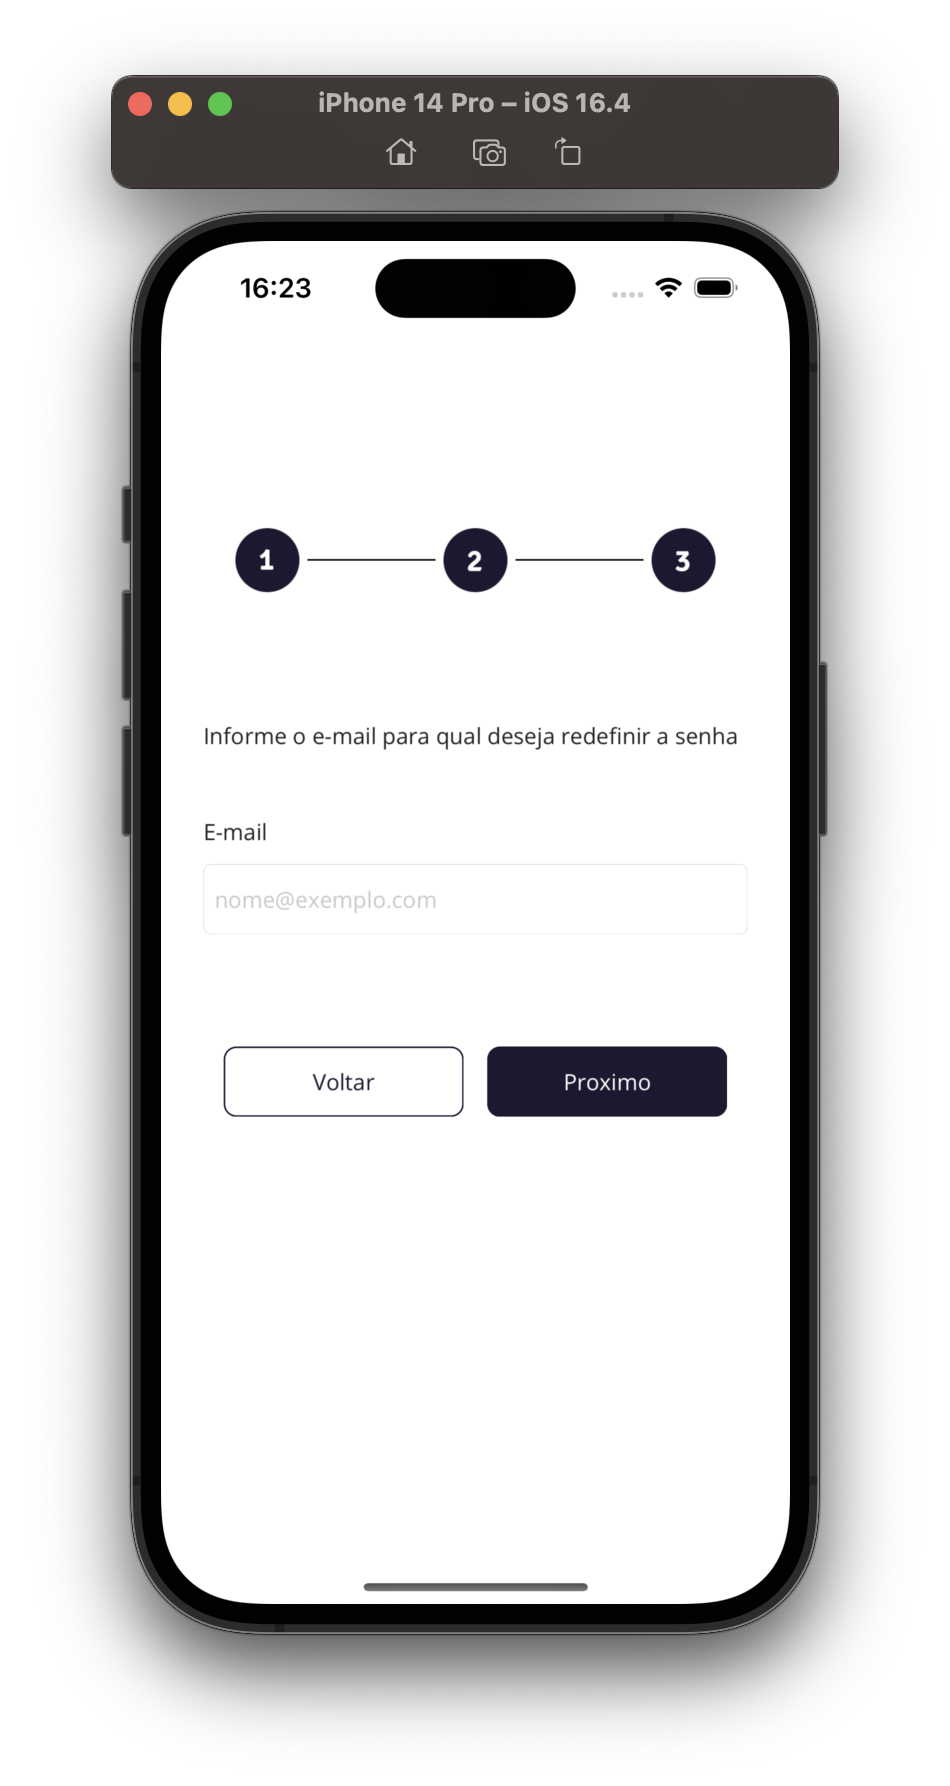
\includegraphics[scale=0.2]{figs/figura30.png}
            \captionof{figure}{Esqueci a Senha I}
            \label{fig:figura30}
        \end{minipage}%
        \begin{minipage}{0.4\textwidth}
            \centering
            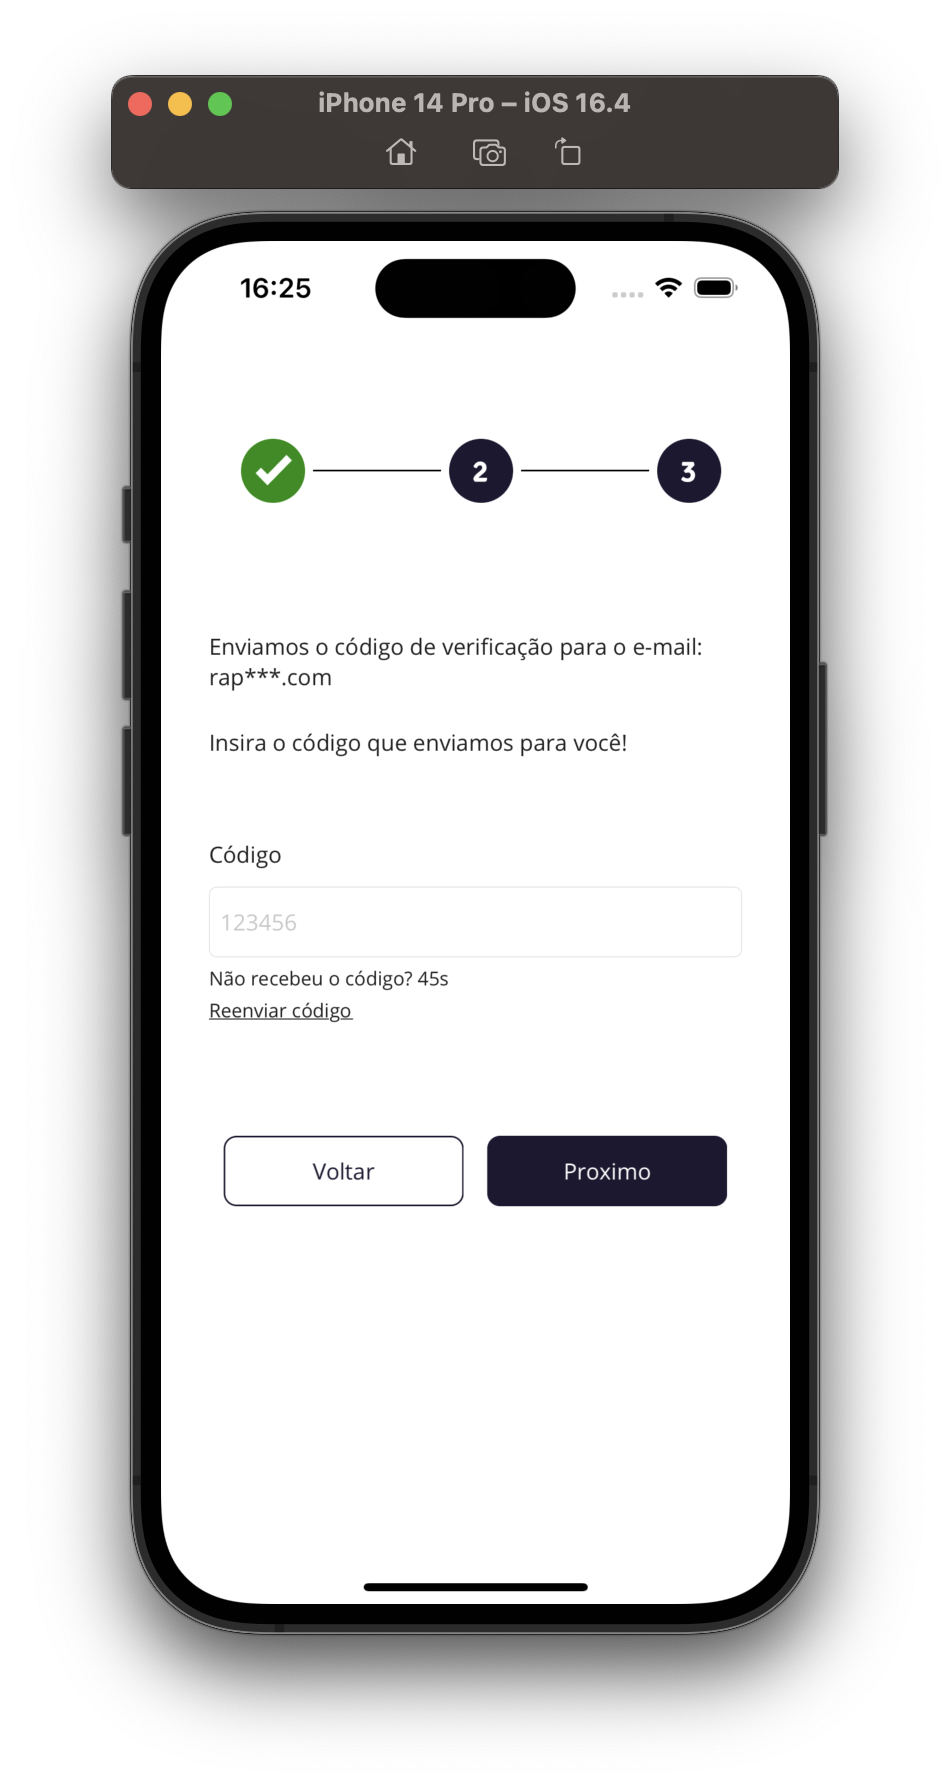
\includegraphics[scale=0.2]{figs/figura31.png}
            \captionof{figure}{Esqueci a Senha II}
            \label{fig:figura31}
        \end{minipage}%
    \end{center}

Consequentemente, uma nova tela aparecerá, contendo um campo para inserir um código que será enviado para o \textit{e-mail} correspondente. Basta inserir esse código no campo e clicar em \textbf{“Verificar”} para confirmar. Caso não tenha recebido o código no \textit{e-mail}, é possível reenviar clicando em \textbf{“Reenviar Código”}, disponível a cada 45 segundos. Na figura 32 e 33, é apresentado a tela de senha redefinida.

    \begin{center}
        \begin{minipage}{0.4\textwidth}
            \centering
            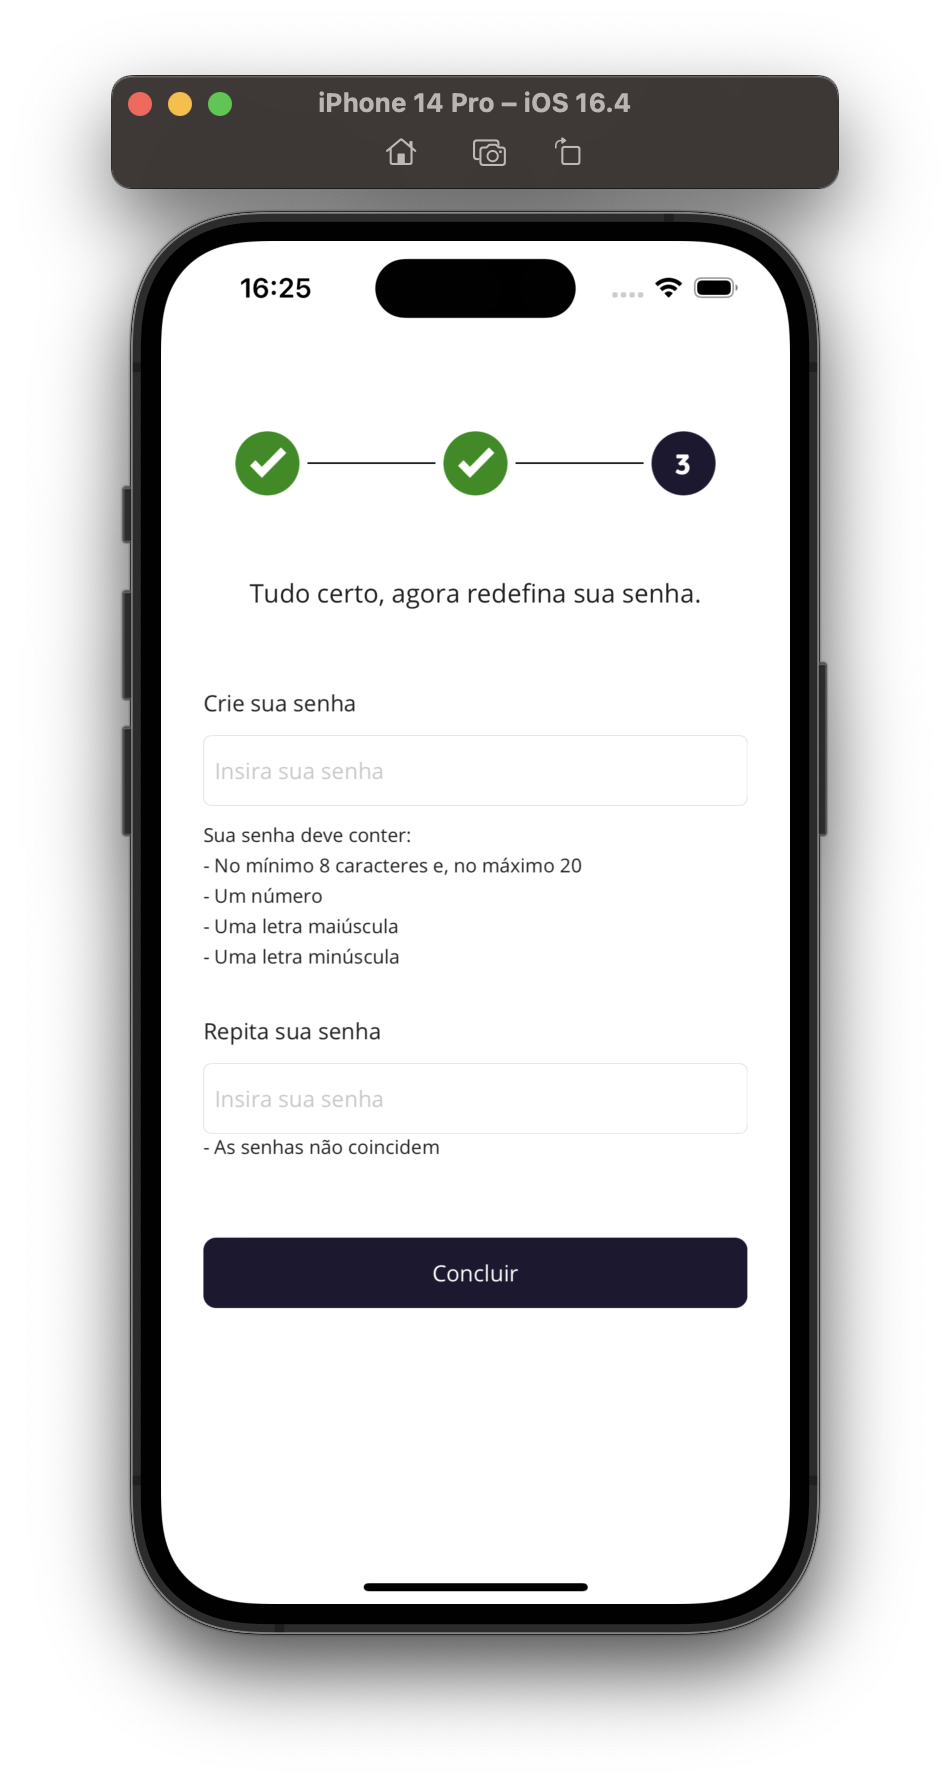
\includegraphics[scale=0.2]{figs/figura32.png}
            \captionof{figure}{Esqueci a Senha III}
            \label{fig:figura32}
        \end{minipage}%
        \begin{minipage}{0.4\textwidth}
            \centering
            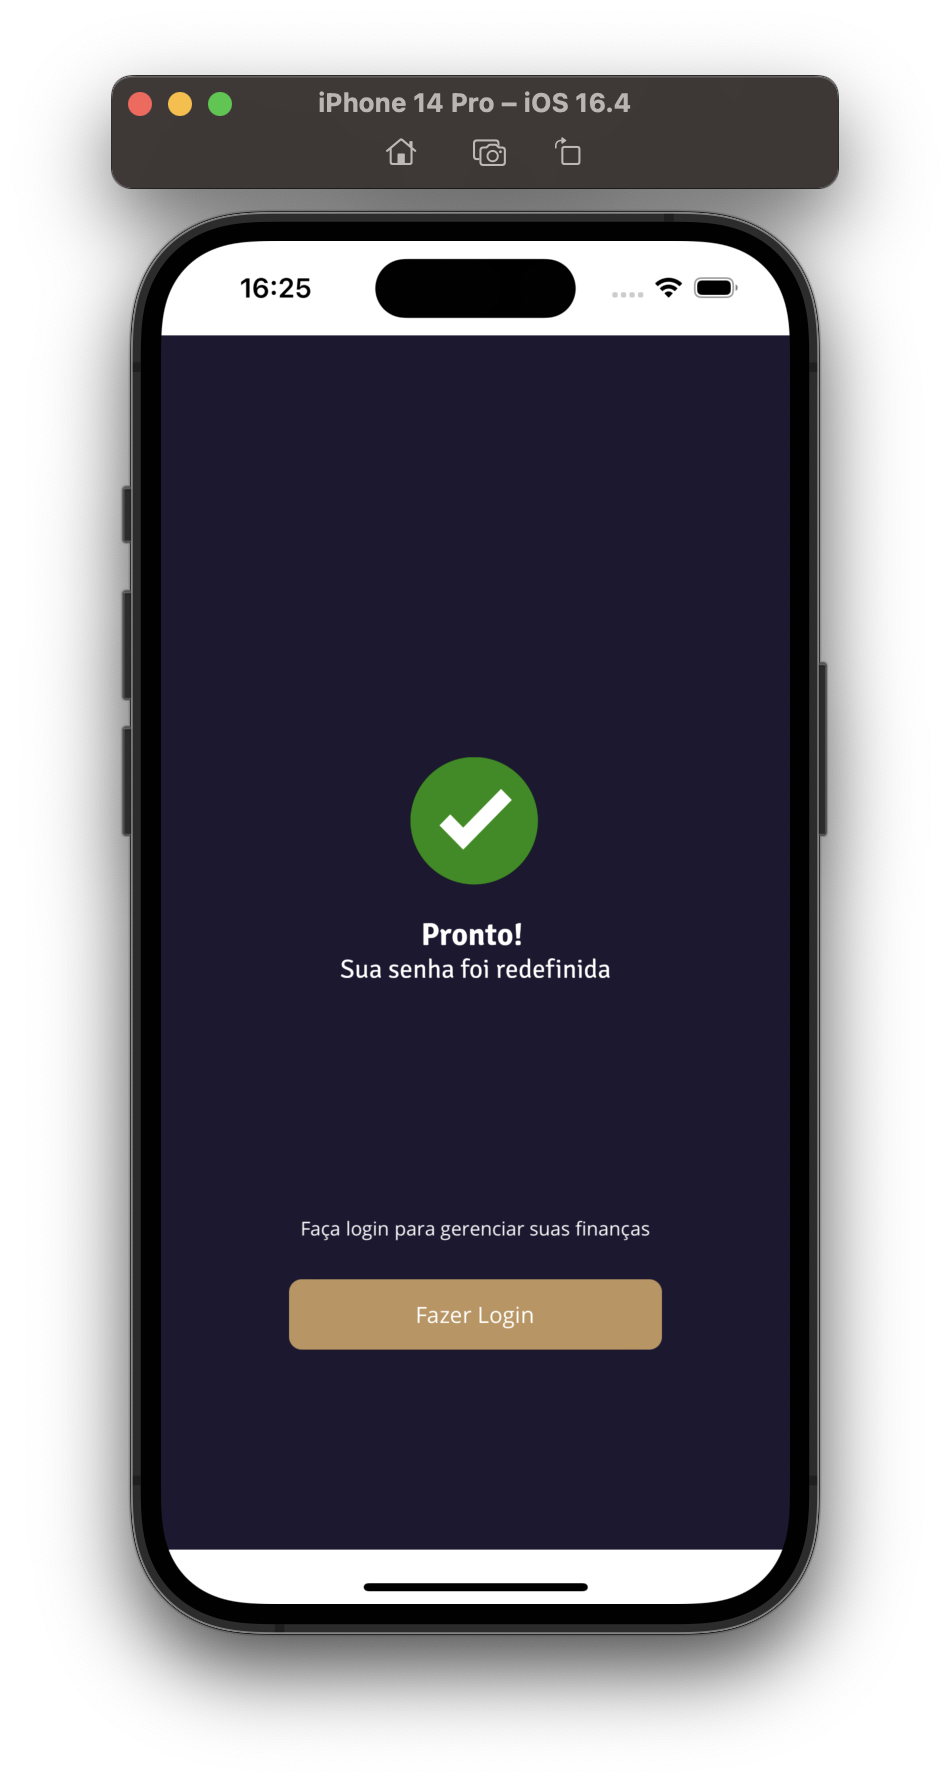
\includegraphics[scale=0.2]{figs/figura33.png}
            \captionof{figure}{Esqueci a Senha IV}
            \label{fig:figura33}
        \end{minipage}%
    \end{center}

Ao clicar um novo código será enviado. Após verificar o código e ter sucesso, uma nova tela surgirá contendo campos para redefinição de senha, o primeiro campo é destinado para inserção da nova senha, que deve respeitar as seguintes exigências: conter no mínimo 8 caracteres, um número, uma letra maiúscula, uma letra minúscula. No campo abaixo repita sua senha caso ambas estejam idênticas clique em \textbf{“Próximo”}. E uma tela apontando sucesso na ação vira à tona, conforme descrito na figura 32. Na figura 34 é apresentada um exemplo da mensagem do código de verificação enviado através do \textit{email}.

    \vspace{\baselineskip}
    \begin{center}
        \begin{minipage}{\textwidth}
            \centering
            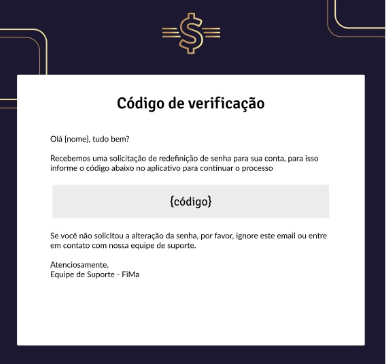
\includegraphics[scale=0.6]{figs/img_6_1.png}
            \captionof{figure}{Esqueci a Senha V}
            \label{fig:figura33}
        \end{minipage}
    \end{center}   

Ao solicitar uma redefinição de senha, a tela acima será exibida, apresentando um campo que requer um código, o qual é gerado através aplicativo. Isso adiciona uma camada adicional às ações. Se não houve solicitação de redefinição de senha, ignore o \textit{e-mail} ou entre em contato com a equipe de suporte.

\subsection{Código Fonte}

Código fonte do projeto: \href{https://github.com/raphaelfrei/financial-manager}{https://github.com/raphaelfrei/financial-manager}

Código fonte do LaTeX: \href{https://github.com/raphaelfrei/fima-final_paper}{https://github.com/raphaelfrei/fima-final\_paper}
% ----------------------------------------------------------
% Testes
% 
% ----------------------------------------------------------

\chapter[Testes]{Testes}

Nesse capitulo, são descritos os planejamentos de testes, com a descrição de todos os casos de testes envolvidos na aplicação.

\section{Planos de Testes}

Para uma melhor eficácia dos testes, é de suma importância o planejamento dos testes, no desenvolvimento de software é imprescindível para o projeto ser bem sucedido. De acordo com o grande crescimento e avanço tecnológico se torna cada vez mais necessário entregar softwares seguros, de altíssima qualidade e confiáveis torna-se uma prioridade absoluta. 
Após todas as telas serem finalizadas, começamos a planejar os testes necessários para entregar um software com um ótimo funcionamento, o primeiro teste realizado foi no sistema de login, no qual, testamos a criação da conta, a redefinição da senha e o login no aplicativo. No segundo teste, verificamos o menu principal, no qual foram analisados os controles de receita, os controles de despesas e a importação da fatura em PDF. 


\section{Cenários de Testes}

\subsection{Sistema de Login}

Testes realizados para testar e validar o funcionamento do sistema de login e dos subprogramas.

\vspace{\baselineskip}
\vspace{\baselineskip}
\vspace{\baselineskip}
\vspace{\baselineskip}
\vspace{\baselineskip}
\vspace{\baselineskip}
\vspace{\baselineskip}
\vspace{\baselineskip}
\vspace{\baselineskip}
\vspace{\baselineskip}
\vspace{\baselineskip}

\subsubsection{Caso de Teste 0001 - Realizar Login}

Teste realizado para a validação de usuário e senha a partir do menu principal, conforme figura 35.

    \begin{center}
        \begin{minipage}{\textwidth}
            \centering
            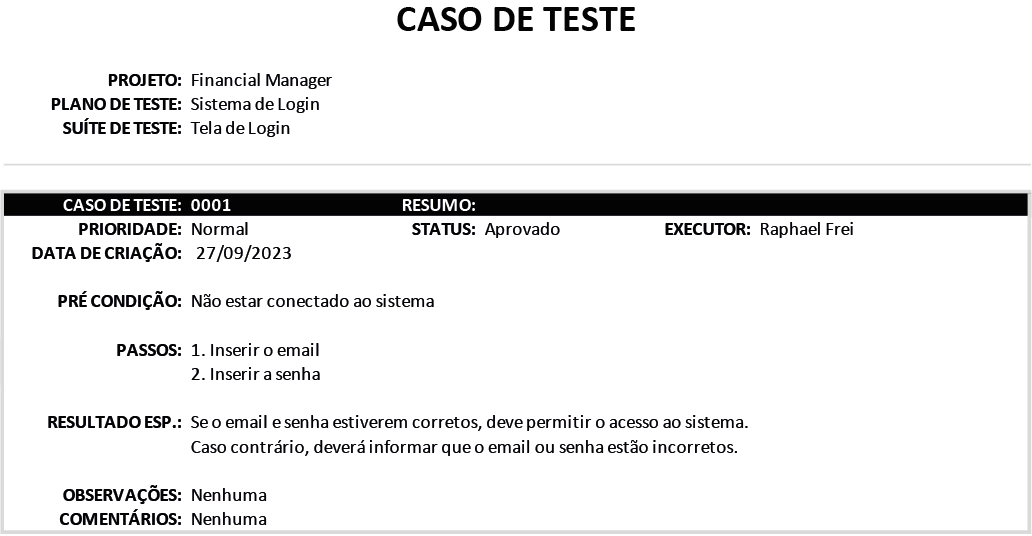
\includegraphics[scale=0.8]{figs/caso-testes-0001.png}
            \captionof{figure}{Caso de Teste da Tela de Login}
            \label{fig:figura35}
        \end{minipage}
    \end{center} 

\subsubsection{Caso de Teste 0002 - Recuperar a Senha}

Teste realizado para a recuperação de senha do usuário, conforme figura 36.

    \begin{center}
        \begin{minipage}{\textwidth}
            \centering
            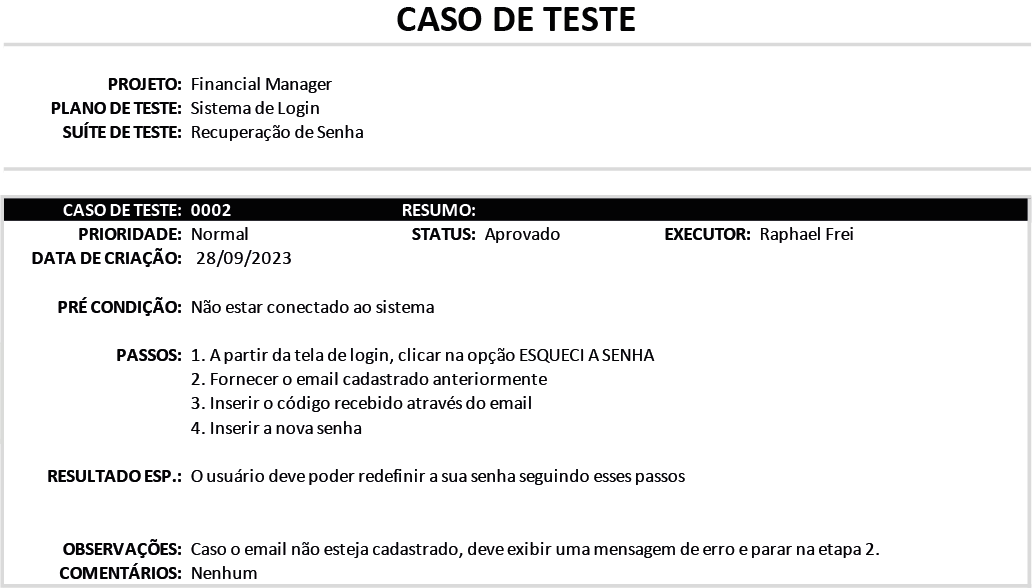
\includegraphics[scale=0.8]{figs/caso-testes-0002.png}
            \captionof{figure}{Caso de Teste da Recuperação de Senha}
            \label{fig:figura36}
        \end{minipage}
    \end{center} 

\subsubsection{Caso de Teste 0003 - Cadastro de Conta}

Teste realizado para o cadastro de novas contas, descrito na figura 37.

    \begin{center}
        \begin{minipage}{\textwidth}
            \centering
            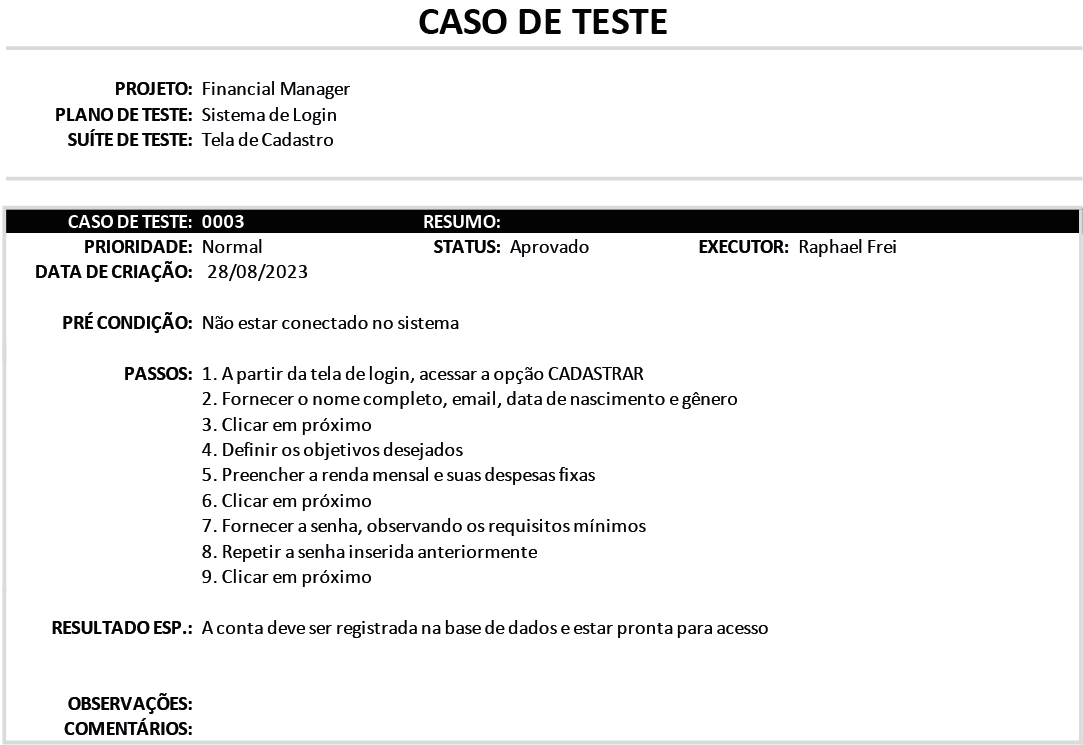
\includegraphics[scale=0.8]{figs/caso-testes-0003.png}
            \captionof{figure}{Caso de Teste da Tela de Cadastro}
            \label{fig:figura37}
        \end{minipage}
    \end{center} 

\subsubsection{Caso de Teste 0004 - Recuperar Conta}

Teste realizado para o processo de recuperação do acesso, descrito na figura 38.

    \begin{center}
        \begin{minipage}{\textwidth}
            \centering
            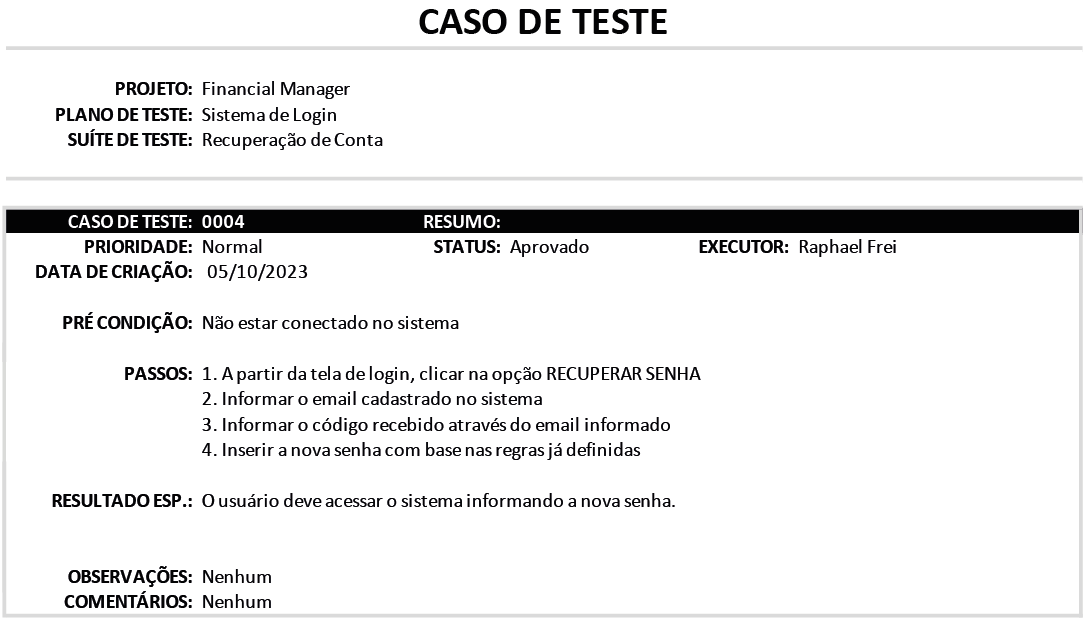
\includegraphics[scale=0.75]{figs/caso-testes-0004.png}
            \captionof{figure}{Caso de Teste da Recuperação de Conta}
            \label{fig:figura38}
        \end{minipage}
    \end{center} 
    
\subsection{Menu Principal}

Teste realizado para testar e validar o funcionamento do menu principal e dos subprogramas.

\subsubsection{Caso de Teste 0005 - Adicionar Receita}

Teste realizado para a tela de adição de receitas, descrito na figura 39.

    \begin{center}
        \begin{minipage}{\textwidth}
            \centering
            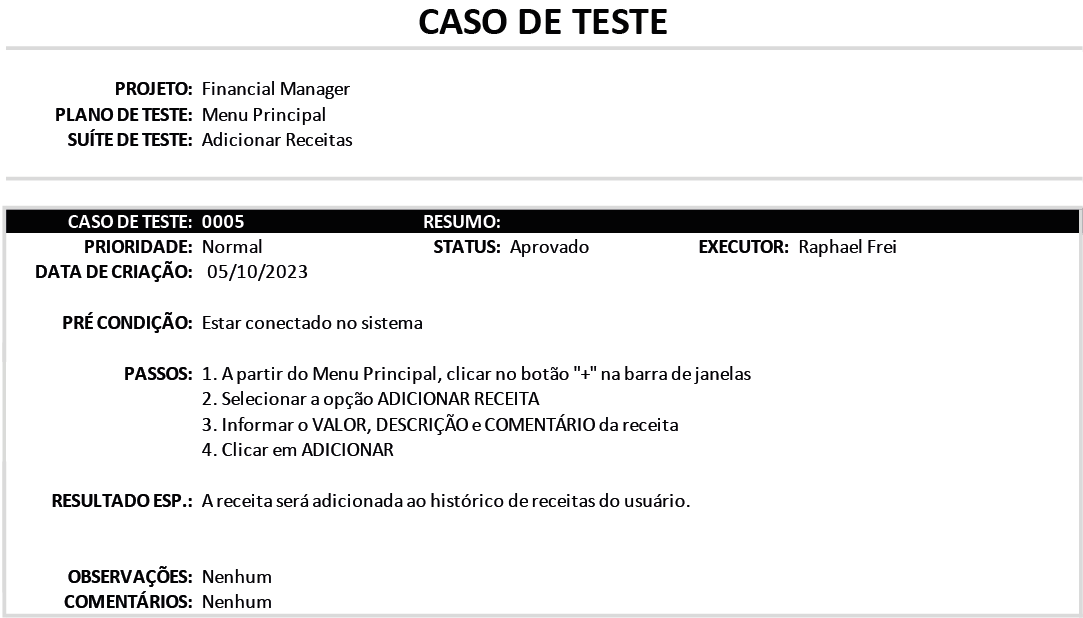
\includegraphics[scale=0.8]{figs/caso-testes-0005.png}
            \captionof{figure}{Caso de Teste para Adicionar Receita}
            \label{fig:figura39}
        \end{minipage}
    \end{center} 

\subsubsection{Caso de Teste 0006 - Editar Receita}

Teste realizado para a tela de edição de receitas, conforme figura 40.

    \begin{center}
        \begin{minipage}{\textwidth}
            \centering
            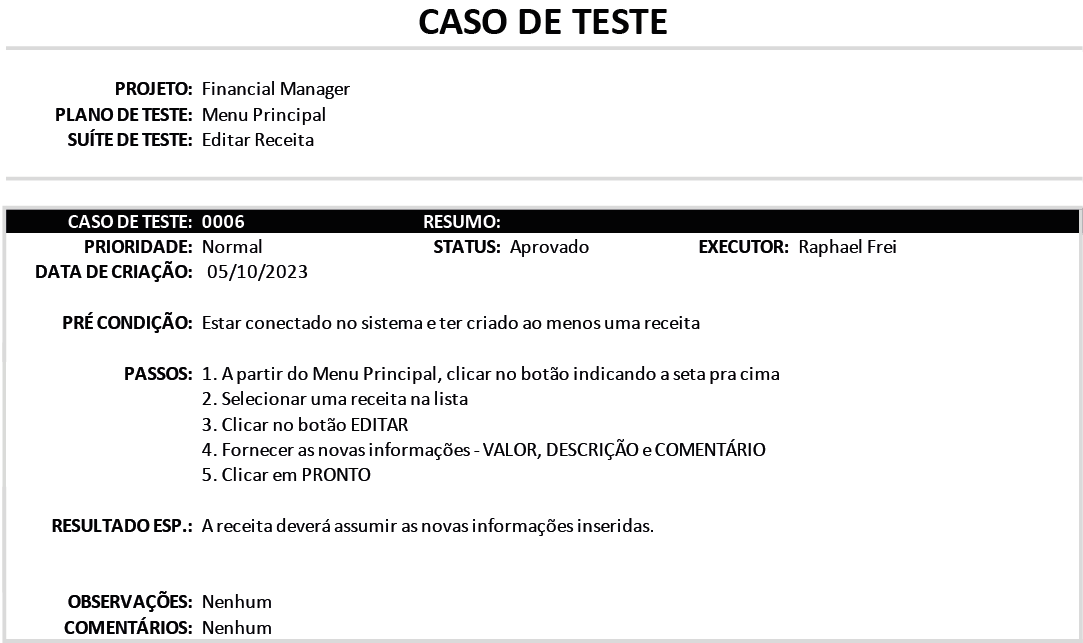
\includegraphics[scale=0.5]{figs/caso-testes-0006.png}
            \captionof{figure}{Caso de Teste para Editar Receita}
            \label{fig:figura40}
        \end{minipage}
    \end{center} 

\subsubsection{Caso de Teste 0007 - Excluir Receita}

Teste realizado para a tela de exclusão de receitas, conforme figura 41.

    \begin{center}
        \begin{minipage}{\textwidth}
            \centering
            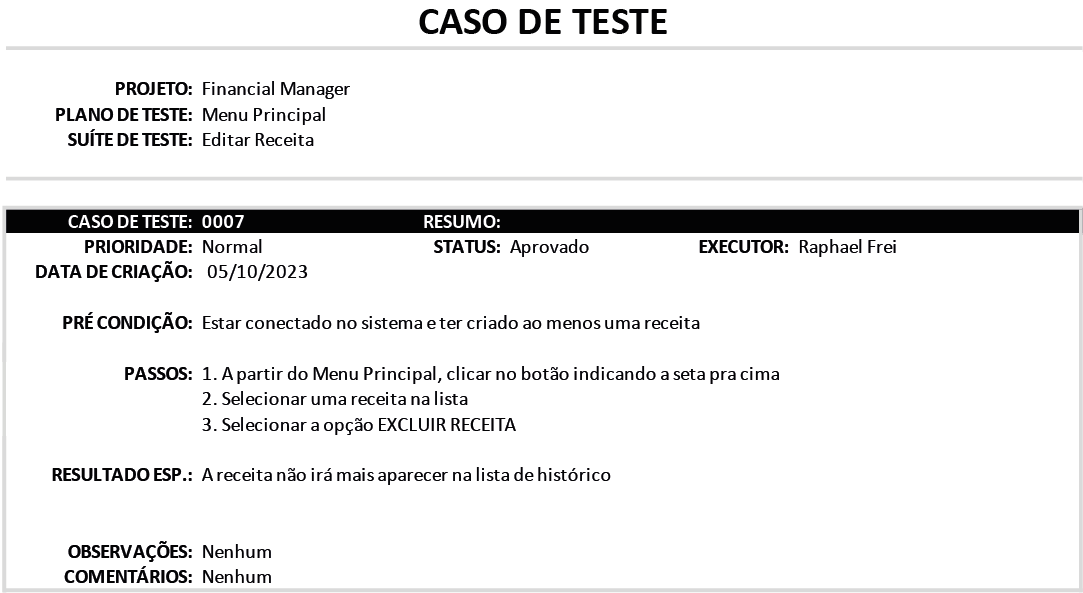
\includegraphics[scale=0.8]{figs/caso-testes-0007.png}
            \captionof{figure}{Caso de Teste para Excluir Receita}
            \label{fig:figura41}
        \end{minipage}
    \end{center} 

\subsubsection{Caso de Teste 0008 - Importar PDF}

Teste realizado para o sistema de importação de fatura em PDF, conforme figura 42.

    \begin{center}
        \begin{minipage}{\textwidth}
            \centering
            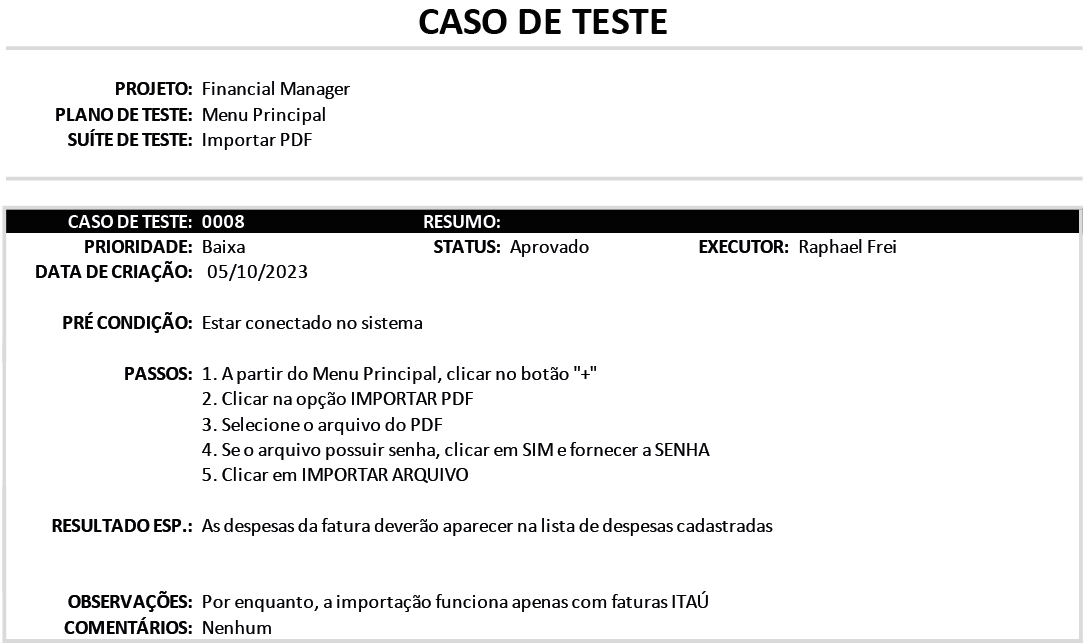
\includegraphics[scale=0.8]{figs/caso-testes-0008.png}
            \captionof{figure}{Caso de Teste para Importar PDF}
            \label{fig:figura42}
        \end{minipage}
    \end{center} 

\subsubsection{Caso de Teste 0009 - Adicionar Despesa}

Teste realizado para a tela de adição de despesas, conforme figura 43.

    \begin{center}
        \begin{minipage}{\textwidth}
            \centering
            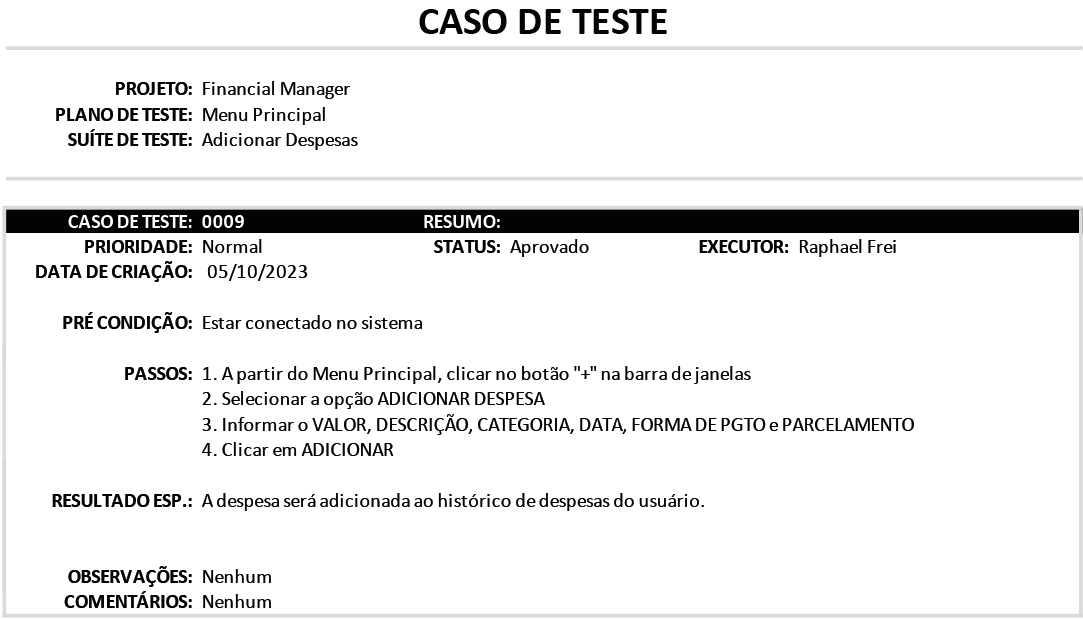
\includegraphics[scale=0.8]{figs/caso-testes-0009.png}
            \captionof{figure}{Caso de Teste para Adicionar Despesa}
            \label{fig:figura43}
        \end{minipage}
    \end{center} 

\subsubsection{Caso de Teste 0010 - Editar Despesa}

Teste realizado para a tela de edição de despesas, conforme figura 44.

    \begin{center}
        \begin{minipage}{\textwidth}
            \centering
            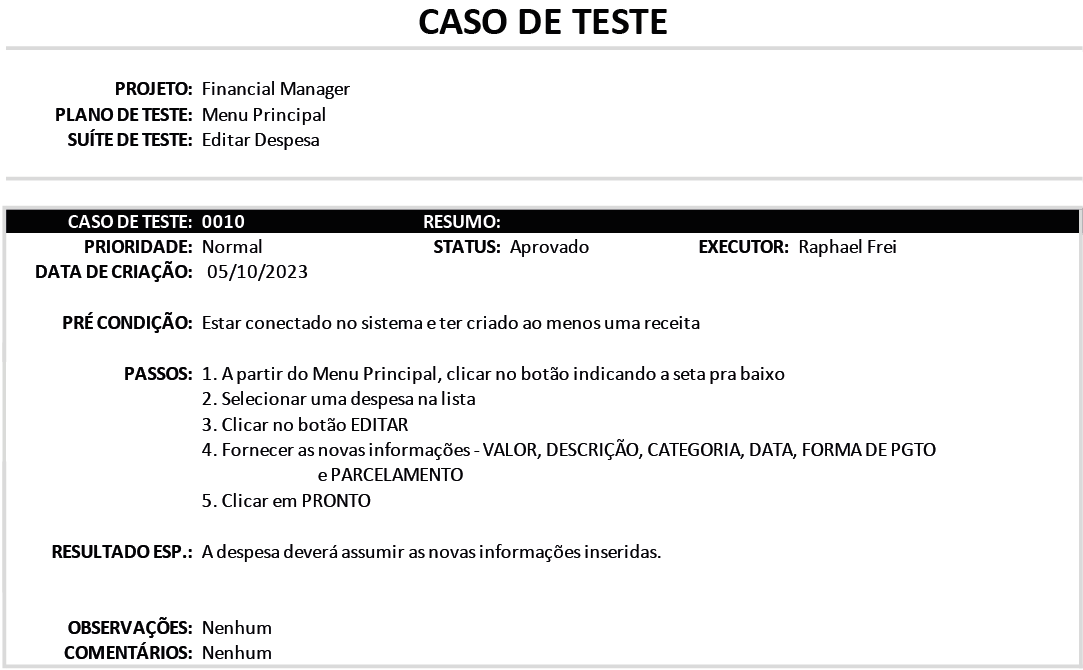
\includegraphics[scale=0.8]{figs/caso-testes-0010.png}
            \captionof{figure}{Caso de Teste para Editar Despesa}
            \label{fig:figura44}
        \end{minipage}
    \end{center} 

\subsubsection{Caso de Teste 0011 - Excluir Despesa}

Teste realizado para a tela de exclusão de despesas, conforme figura 45.

    \begin{center}
        \begin{minipage}{\textwidth}
            \centering
            \includegraphics[scale=0.8]{figs/caso-testes-0011.png}
            \captionof{figure}{Caso de Teste para Excluir Despesa}
            \label{fig:figura45}
        \end{minipage}
    \end{center} 

% ----------------------------------------------------------
% Considerações Finais
% 
% ----------------------------------------------------------

\chapter[Resultados finais]{Resultados Finais}

O presente trabalho adota uma abordagem de finalização que se baseia em um protótipo, ou seja, uma representação do produto final que tem como finalidade proporcionar uma experiência imersiva do aplicativo, sendo assim, os usuários poderão interagir dentro dele e conhecer na prática sua proposta. O projeto foi organizado por uma série de etapas planejadas, cada uma representando um marco significativo em nossa jornada a uma conclusão bem-sucedida. A primeira etapa foi da pesquisa bibliográfica, possibilitando maior conhecimento sobre os temas da pesquisa. A segunda foi a pesquisa de cunho quantitativo com possíveis usuários, a partir dos dados obtidos através da realização da pesquisa, foi possível planejar nosso projeto de forma mais assertiva para atender a necessidade de todos os usuários e viabilizar uma melhor experiência. Em seguida a criação do logo, paleta de cores, primeiras telas do aplicativo no Figma, início do desenvolvimento dos códigos e primeiras interações com o aplicativo funcionando. 

O plano de teste foi pensado estritamente para analisar os principais casos e possíveis erros, um componente essencial e estratégico para assegurar a qualidade e confiabilidade do projeto em questão. Portanto, a partir dos testes planejados e executados, os erros apresentados inicialmente puderam ser corrigidos, logo concluímos essa fase com êxito.
O desenvolvimento deste trabalho foi uma etapa crucial, onde se tornou evidente a aplicação prática das teorias e métodos propostos inicialmente. Ao longo deste processo, nosso principal objetivo foi criar um aplicativo para ajudar pessoas que estão buscando uma maneira mais fácil e prática para organizar sua vida financeira, além de contribuir com a transformação que tem ocorrido no mercado financeiro. Para a construção do design de interfaces utilizamos o Figma (UX/UI), para a criação da tela (\textit{Front End}) foi utilizado o .NET MAUI e para implementar suas funcionalidades (\textit{Back End}) o C\#. 

Nosso Ambiente de desenvolvimento Integrado (IDE) foi o Visual Studio, Android Studio, que é um emulador Android, no qual simula um celular com o sistema operacional Android e o XCode no qual simula um celular com sistema operacional iOS, da Apple. O principal desafio enfrentado por nossa equipe, foi desenvolvendo as telas do aplicativo, no qual estávamos utilizando o programa Unity para realizar este processo, porém após finalizar desenvolvimentos sempre nos deparávamos com erros e problemas de comunicação entre as telas assim optando por trocar toda a linguagem \textit{Front End} da aplicação durante o TCC. 

Ao finalizar este projeto, é evidente que cada etapa percorrida contribuiu de maneira significativa para o alcance dos objetivos propostos. O resultado obtido como a finalização do protótipo totalmente funcional, não apenas valida todos os objetivos apontados desde o início, mas também revelam oportunidades de aprimoramento e desenvolvimento futuros. Assim como, a integração do \textit{Open Banking} ao aplicativo, para termos atualizações em tempo real da conta bancária de nossos usuários, aulas sobre finanças com professores qualificados para um melhor entendimento sobre como utilizar seu dinheiro, aulas sobre investimento e ser possível acessar e desbloquear o aplicativo através da biometria cadastrada no dispositivo.

A idealização para a continuidade do projeto seria abrir oportunidade para patrocinadores que gostariam de anunciar suas aulas e possivelmente integrarmos com o Google ADS para anúncios personalizados para cada usuário. Um outro planejamento é existir versões pagas que faz com que não apareçam anúncios para os usuários. Temos uma boa equipe com capacidade de desenvolvimento para fazer com que o projeto não fique apenas com uma prototipação e sim com um aplicativo de fato lançado. Para o projeto se tornar comercial faltam alguns tópicos, um exemplo disso é o que foi citado anteriormente, possibilidade de anúncios no aplicativo, planos pagos pelos usuários, implementação de níveis de segurança melhores, identificação com biometria e muito mais.

Além disso, as lições aprendidas ao longo do caminho se revelaram inestimáveis, mas também muito valiosas para a vida, bem como, trabalho em equipe, gerenciamento de tempo, comprometimento e responsabilidade, gestão de conflitos, adaptações e flexibilidade.


%%%%%%%%%%%%%%%%%%%%%%%%%%%%%%%%%%%%%%%%%%%%%%%%%%%%%%%%%%%%%%%%
%% ELEMENTOS PÓS-TEXTUAIS (Referências, Glossário, Apêndices) %%
%%%%%%%%%%%%%%%%%%%%%%%%%%%%%%%%%%%%%%%%%%%%%%%%%%%%%%%%%%%%%%%%
\postextual

% Referências bibliográficas
\bibliography{bibliografia}

% Apêndices
% ----------------------------------------------------------
% Apêndices
% ----------------------------------------------------------

% ---
% Inicia os apêndices
% ---
\begin{apendicesenv}

% Imprime uma página indicando o início dos apêndices
\partapendices

% ----------------------------------------------------------
\chapter{Roteiro de Entrevista}
% ----------------------------------------------------------

Neste apêndice, apresentamos o Roteiro de Entrevista que foi utilizado como parte fundamental da pesquisa realizada para este Trabalho de Conclusão de Curso. A pesquisa concentrou-se na análise do meio financeiro de um grupo específico de indivíduos, e o roteiro de entrevista desempenhou um papel central na coleta de dados necessários para alcançar os objetivos deste estudo. Durante essa pesquisa, obtivemos 380 respostas.

O roteiro de entrevista foi projetado com o propósito de obter informações valiosas sobre as experiências, percepções e comportamentos financeiros dos participantes. Esta seção descreverá o conteúdo do roteiro, sua estrutura e como ele foi aplicado durante o processo de coleta de dados. Além disso, apresentaremos as questões-chave que foram incluídas no roteiro para que os leitores possam compreender o contexto e a abordagem utilizados para investigar o tema em questão.

É importante notar que a elaboração cuidadosa do roteiro de entrevista desempenhou um papel crucial na qualidade dos dados coletados e na robustez das conclusões tiradas a partir da pesquisa. 

A seguir, apresentamos, em detalhes, o roteiro utilizado neste estudo.

\begin{table}[ht]
    \centering
    \setlength{\extrarowheight}{3pt}  % Aumenta a altura das linhas da tabela

    \begin{center}
        \begin{minipage}{\textwidth}
            \centering
            \begin{tabular}{|c|c|c|}
                \textbf{Faixa Etária} & \textbf{Total Respondentes} & \textbf{Percentual} \\
                Até 18 anos & 67 pessoas & 17,6\% \\
                Entre 19 e 22 anos & 188 pessoas & 49,5\% \\
                Entre 23 e 25 anos & 51 pessoas & 13,4\% \\
                Entre 26 e 30 anos & 35 pessoas & 9,2\% \\
                Mais de 31 anos & 39 pessoas & 10,3\%
            \end{tabular}
        \end{minipage}
    \end{center}

    \caption{Qual a Idade dos Respondentes?}
    \label{tab:idade}
\end{table}

\begin{table}[ht]
    \centering
    \setlength{\extrarowheight}{3pt}  % Aumenta a altura das linhas da tabela

    \begin{center}
        \begin{minipage}{\textwidth}
            \centering
            \begin{tabular}{|c|c|c|}
                \textbf{Tipo da Cidade} & \textbf{Total Respondentes} & \textbf{Percentual} \\
                Grande & 317 pessoas & 83,4\% \\
                Pequena e Média & 61 pessoas & 16,1\% \\
                Rural & 2 pessoas & 0,5\% \\
            \end{tabular}
        \end{minipage}
    \end{center}

    \caption{Em qual região mora?}
    \label{tab:regiao}
\end{table}

\begin{table}[ht]
    \centering
    \setlength{\extrarowheight}{3pt}  % Aumenta a altura das linhas da tabela

    \begin{center}
        \begin{minipage}{\textwidth}
            \centering
            \begin{tabular}{|c|c|c|}
                \textbf{Formação Acadêmica} & \textbf{Total Respondentes} & \textbf{Percentual} \\
                Fundamental Completo & 4 pessoas & 1,1\% \\
                Ensino Médio Completo & 218 pessoas & 73,2\% \\
                Graduação Completa & 80 pessoas & 21,1\% \\
                Pós Graduado & 17 pessoas & 4,5\% \\
                Doutorando & 1 pessoa & 0,3\% \\
            \end{tabular}
        \end{minipage}
    \end{center}

    \caption{Qual a formação atual?}
    \label{tab:formacao}
\end{table}

\begin{table}[ht]
    \centering
    \setlength{\extrarowheight}{3pt}  % Aumenta a altura das linhas da tabela

    \begin{center}
        \begin{minipage}{\textwidth}
            \centering
            \begin{tabular}{|c|c|c|}
                \textbf{Faixa de Renda} & \textbf{Total Respondentes} & \textbf{Percentual} \\
                Até R\$ 1.300 & 74 pessoas & 19\% \\
                Entre R\$ 1.301 até R\$1.800 & 57 pessoas & 15\% \\
                Entre R\$ 1.801 até R\$2.500 & 52 pessoas & 13,7\% \\
                Entre R\$ 2.501 até R\$3.500 & 38 pessoas & 10\% \\
                Entre R\$ 3.501 até R\$5.000 & 20 pessoas & 5,3\% \\
                Mais que R\$5.001 & 47 pessoas & 12,4\% \\
                Preferiu não revelar & 93 pessoas & 24,2\% \\
            \end{tabular}
        \end{minipage}
    \end{center}

    \caption{Qual a renda atual?}
    \label{tab:renda}
\end{table}

\begin{table}[ht]
    \centering
    \setlength{\extrarowheight}{3pt}  % Aumenta a altura das linhas da tabela

    \begin{center}
        \begin{minipage}{\textwidth}
            \centering
            \begin{tabular}{|c|c|c|}
                \textbf{Situação} & \textbf{Total Respondentes} & \textbf{Percentual} \\
                Negativo & 59 pessoas & 15,5\% \\
                Equilibrado & 235 pessoas & 61,8\% \\
                Positivo & 86 pessoas & 22,6\% \\
            \end{tabular}
        \end{minipage}
    \end{center}

    \caption{Como avalia sua situação financeira?}
    \label{tab:situacao}
\end{table}

\begin{table}[ht]
    \centering
    \setlength{\extrarowheight}{3pt}  % Aumenta a altura das linhas da tabela

    \begin{center}
        \begin{minipage}{\textwidth}
            \centering
            \begin{tabular}{|c|c|c|}
                \textbf{Situação} & \textbf{Total Respondentes} & \textbf{Percentual} \\
                Alto & 30 pessoas & 7,9\% \\
                Média & 240 pessoas & 63,2\% \\
                Baixo & 110 pessoas & 28,9\% \\
            \end{tabular}
        \end{minipage}
    \end{center}

    \caption{Como avalia seu conhecimento financeiro?}
    \label{tab:educacaofinanceira}
\end{table}

\begin{table}[ht]
    \centering
    \setlength{\extrarowheight}{3pt}  % Aumenta a altura das linhas da tabela

    \begin{center}
        \begin{minipage}{\textwidth}
            \centering
            \begin{tabular}{|c|c|c|}
                \textbf{Possui Crédito} & \textbf{Total Respondentes} & \textbf{Percentual} \\
                Sim & 259 pessoas & 68,2\% \\
                Não & 121 pessoas & 31,8\% \\
            \end{tabular}
        \end{minipage}
    \end{center}

    \caption{Você possui algum tipo de crédito bancário?}
    \label{tab:pscredito}
\end{table}

\begin{table}[ht]
    \centering
    \setlength{\extrarowheight}{3pt}  % Aumenta a altura das linhas da tabela

    \begin{center}
        \begin{minipage}{\textwidth}
            \centering
            \begin{tabular}{|c|c|c|}
                \textbf{Tipo de Crédito} & \textbf{Total Respondentes} & \textbf{Percentual} \\
                Cartão de Débito & 216 pessoas & 56,8\% \\
                Cartão de Crédito & 132 pessoas & 34,7\% \\
                Dinheiro & 26 pessoas & 6,8\% \\
                PIX & 6 pessoas & 1,7\% \\
            \end{tabular}
        \end{minipage}
    \end{center}
    
    \caption{Qual a forma de pagamento mais utilizada?}
    \label{tab:pagto}
\end{table}
\
\begin{table}[ht]
    \centering
    \setlength{\extrarowheight}{3pt}  % Aumenta a altura das linhas da tabela

    \begin{center}
        \begin{minipage}{\textwidth}
            \centering
            \begin{tabular}{|c|c|c|}
                \textbf{Tipo de Crédito} & \textbf{Total Respondentes} & \textbf{Percentual} \\
                Sim & 245 pessoas & 64,5\% \\
                Não & 135 pessoas & 35,5\% \\
            \end{tabular}
        \end{minipage}
    \end{center}
    
    \caption{Você se considera organizado?}
    \label{tab:consorg}
\end{table}

\begin{table}[ht]
    \centering
    \setlength{\extrarowheight}{3pt}  % Aumenta a altura das linhas da tabela

    \begin{center}
        \begin{minipage}{\textwidth}
            \centering
            \begin{tabular}{|c|c|c|}
                \textbf{Tipo de Crédito} & \textbf{Total Respondentes} & \textbf{Percentual} \\
                Sim & 163 pessoas & 42,9\% \\
                Não & 134 pessoas & 35,3\% \\
                Talvez & 83 pessoas & 21,8\% \\
            \end{tabular}
        \end{minipage}
    \end{center}
    
    \caption{Você utilizaria um aplicativo para controle financeiro?}
    \label{tab:usarapp}
\end{table}

\begin{table}[ht]
    \centering
    \setlength{\extrarowheight}{3pt}  % Aumenta a altura das linhas da tabela

    \vspace{\baselineskip}
    \vspace{\baselineskip}
    \vspace{\baselineskip}
    \vspace{\baselineskip}
    \vspace{\baselineskip}
    \vspace{\baselineskip}
    \vspace{\baselineskip}
    \vspace{\baselineskip}
    \vspace{\baselineskip}
    \vspace{\baselineskip}
    \vspace{\baselineskip}
    \vspace{\baselineskip}
    \vspace{\baselineskip}
    \vspace{\baselineskip}
    \vspace{\baselineskip}
    \vspace{\baselineskip}
    

\end{table}

\end{apendicesenv}
% ---

% Anexos
%% ----------------------------------------------------------
% Apêndices
% ----------------------------------------------------------

% ---
% Inicia os anexos
% ---
\begin{anexosenv}

% Imprime uma página indicando o início dos anexos
\partanexos

% --------------------------------------
\chapter{Nome do Primeiro Anexo}
% --------------------------------------
\lipsum[30] % Texto qualquer. REMOVER!!



\end{anexosenv}


\end{document}
